\documentclass[12pt]{book}
\usepackage[utf 8]{inputenc}
\usepackage[english]{babel}
\usepackage[IL2]{fontenc}

\usepackage{amsfonts}
\usepackage{amsmath}
\usepackage{amsthm}
\usepackage{amssymb}
\usepackage{epsfig}
\usepackage{color}
\usepackage{url}
\usepackage{graphicx}
\usepackage{float}
\usepackage{dsfont}
\usepackage{pdfpages}
\usepackage{afterpage}
\usepackage{setspace}

\usepackage[toc,page]{appendix}

\usepackage{geometry}
 \geometry{
 a4paper,
 %	total={170mm,257mm},
 left = 3cm,
 top = 2.5cm,
 right = 3cm,
 bottom = 2.5cm
 }
 
 \usepackage[inline]{enumitem}
 \usepackage[font=small,labelfont=bf]{caption}

\author{Matúš Stehlík}

\setlength{\parindent}{0em}
\setlength{\parskip}{.5em}
\renewcommand\baselinestretch{1.05} % riadkovanie jeden a pol


\newtheorem{thm}[equation]{Theorem}
\newtheorem{lema}[equation]{Lemma}
\newtheorem{cor}[equation]{Corollary}
\newtheorem{prop}[equation]{Proposition}
\newtheorem{hyp}[equation]{Hypothesis}
\theoremstyle{definition}
\newtheorem{defi}[equation]{Definition}
%\newtheorem*{proof}{Proof}
\newtheorem{rem}[equation]{Remark}
\newtheorem{ex}[equation]{Example}


% pekne pokope definujeme potrebne udaje
\def\mftitle{Conic Relaxations}
\def\mfthesistype{Diplomová práca}
\def\mfauthor{Bc. Matúš Stehlík}
\def\mfadvisor{RNDr. Mária Trnovská PhD.}
\def\mfplacedate{Bratislava, 2016}

\ifx\pdfoutput\undefined\relax\else\pdfinfo{ /Title (\mftitle) /Author (\mfauthor) /Creator (PDFLaTeX) } \fi

\begin{document}

\frontmatter

\thispagestyle{empty}

\noindent
\begin{minipage}{0.20\textwidth}

\includegraphics[width=0.9\textwidth]{img/komlogo-new.pdf}
\end{minipage}
\begin{minipage}{0.8\textwidth}%{0.79\textwidth}
%\sc Fakulta Matematiky, Fyziky a Informatiky \\
%Univerzita Komenského, Bratislava
\sc Faculty of Mathematics, Physics and Informatics \\
Comenius University, Bratislava
\end{minipage}

\vfill
\begin{center}
\begin{minipage}{0.8\textwidth}
%\hrule
\bigskip\bigskip
\centerline{\LARGE\sc\protect\parbox{1.4\textwidth}{\protect\centering \mftitle}}
\smallskip
\bigskip
\bigskip
\centerline{\large\sc Master's Thesis}
\bigskip\bigskip
%\hrule
\end{minipage}
\end{center}

\vfill
\mfauthor\hfill\mfplacedate
\eject

%%%%%%%%%%%%%%%%%%%%%%%%%%%%%%%%%%%%%%%

\frontmatter

\thispagestyle{empty}

\noindent
\begin{minipage}{0.20\textwidth}

\includegraphics[width=0.9\textwidth]{img/komlogo-new}
\end{minipage}
\begin{minipage}{0.79\textwidth}
\begin{center}
\sc Fakulta Matematiky, Fyziky a Informatiky \\
Univerzita Komenského, Bratislava
\end{center}
\end{minipage}

\vfill
\begin{center}
\begin{minipage}{0.8\textwidth}
%\hrule
\bigskip\bigskip
\centerline{\LARGE\sc\protect\parbox{1.4\textwidth}{\protect\centering Kónické Relaxácie}}
\smallskip
\centerline{(\mfthesistype)}
\bigskip
\bigskip
\centerline{\large\sc\protect\parbox{1.4\textwidth}{\protect\centering \mfauthor}}
\bigskip\bigskip
%\hrule
\end{minipage}
\end{center}
\vfill
\begin{tabular}{ll}
	Študijný program: & Matematika		\\
	Študijný odbor: & 1113 Matematika	\\
	Školiace pracovisko: & Katedra aplikovanej matematiky a štatistiky		\\
	Školiteľ: & RNDr. Mária Trnovská, PhD.	\\
\end{tabular}
\vfill
%\afterpage{\null\newpage}
\hfill\mfplacedate
\eject % EOP i


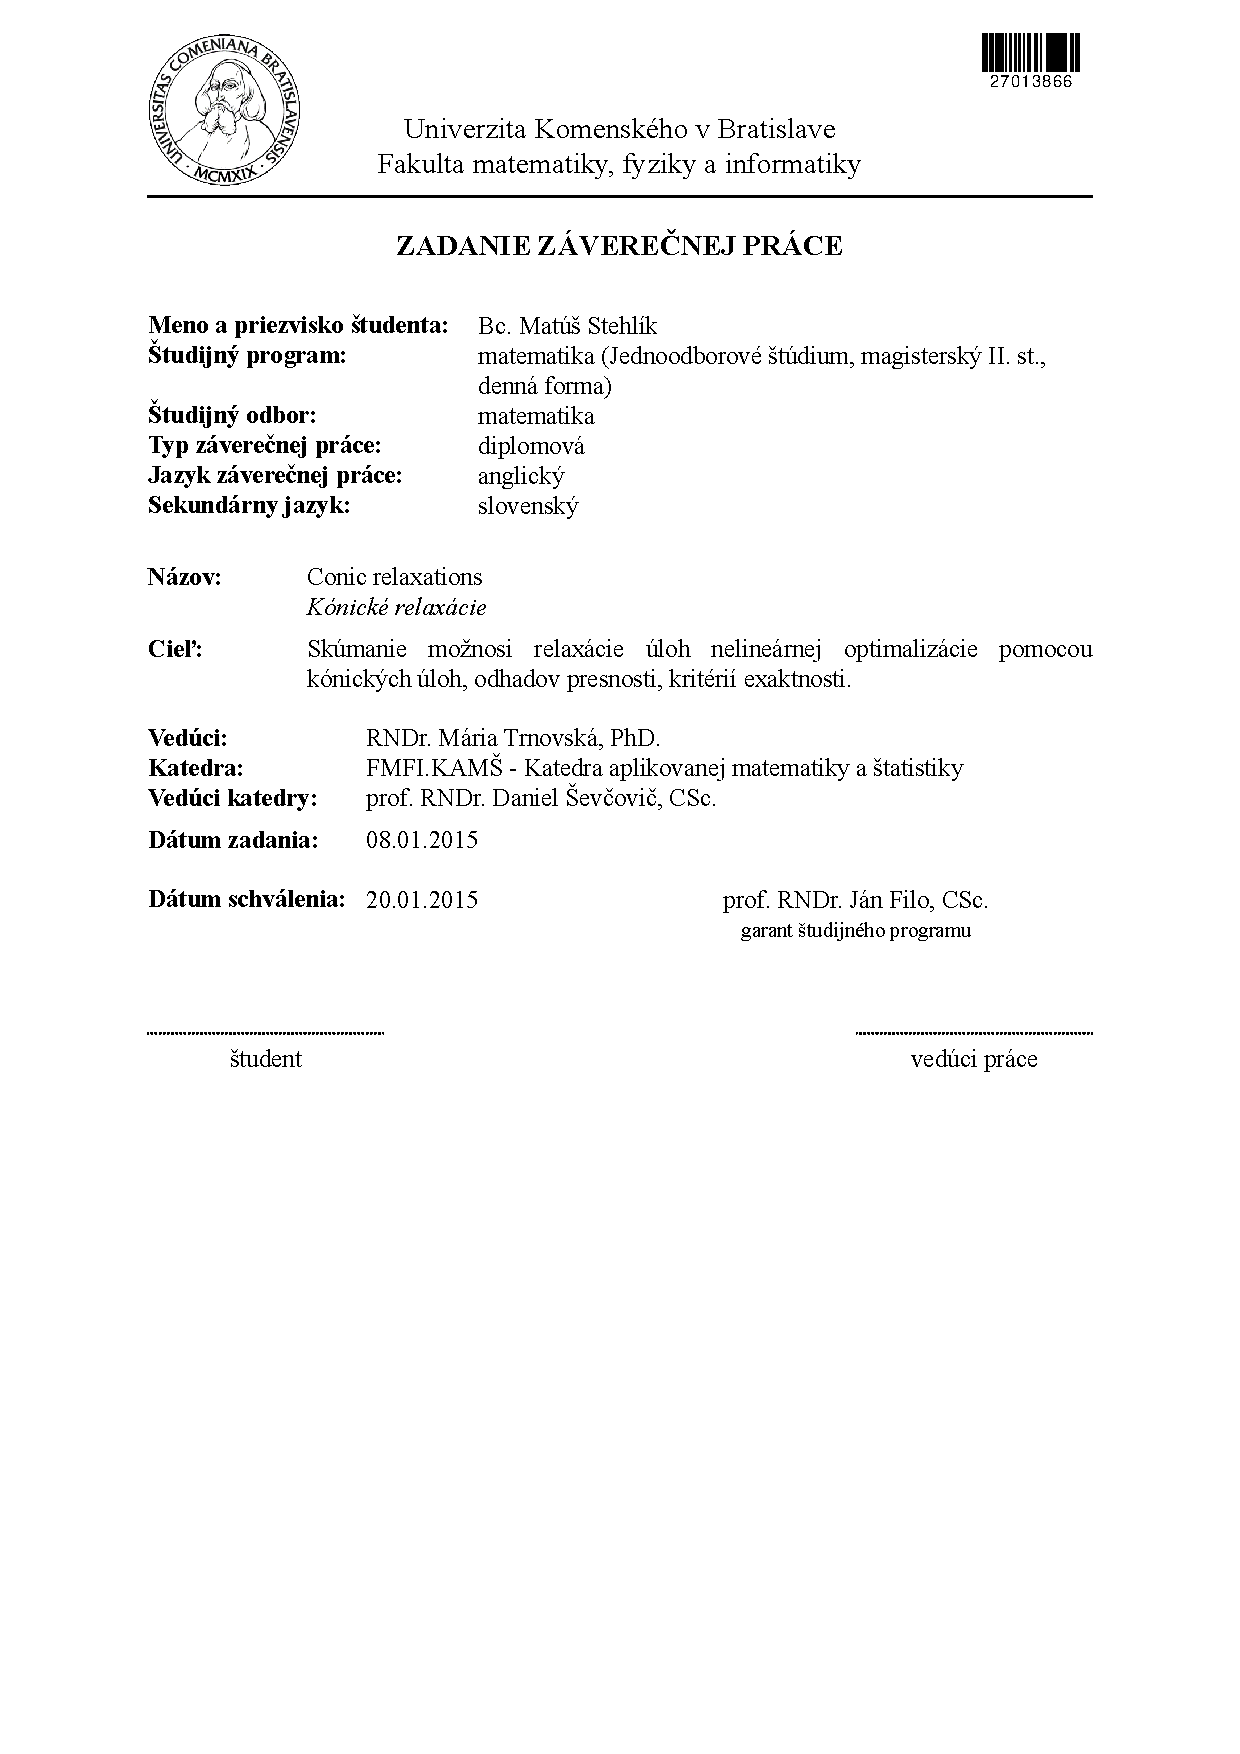
\includepdf{img/zadanie_sk.pdf}
%%%%%%%%%%%%%%%%%%%%
%%%%%%%%%%%%%%%%%%%%%%%%%%%%%%%%%%%%%%%



\thispagestyle{empty}

\noindent
\begin{minipage}{0.20\textwidth}

\includegraphics[width=0.9\textwidth]{img/komlogo-new}
\end{minipage}
\begin{minipage}{0.79\textwidth}
\begin{center}
\sc Faculty of Mathematics, Physics and Informatics\\
Comenius University, Bratislava
\end{center}
\end{minipage}

\vfill
\begin{center}
\begin{minipage}{0.8\textwidth}
%\hrule
\bigskip\bigskip
\centerline{\LARGE\sc\protect\parbox{1.4\textwidth}{\protect\centering Conic Relaxations}}
\smallskip
\centerline{(Master's Thesis)}
\bigskip
\bigskip
\centerline{\large\sc\protect\parbox{1.4\textwidth}{\protect\centering \mfauthor}}
\bigskip\bigskip
%\hrule
\end{minipage}
\end{center}
\vfill
\begin{tabular}{ll}
	Study programme: & Mathematics		\\
	Field of study: & 1113 Mathematics	\\
	Department: & Department of Applied Mathematics and Statistics	\\
	Supervisor: & RNDr. Mária Trnovská, PhD.	\\
\end{tabular}
\vfill

\hfill\mfplacedate
\eject % EOP i


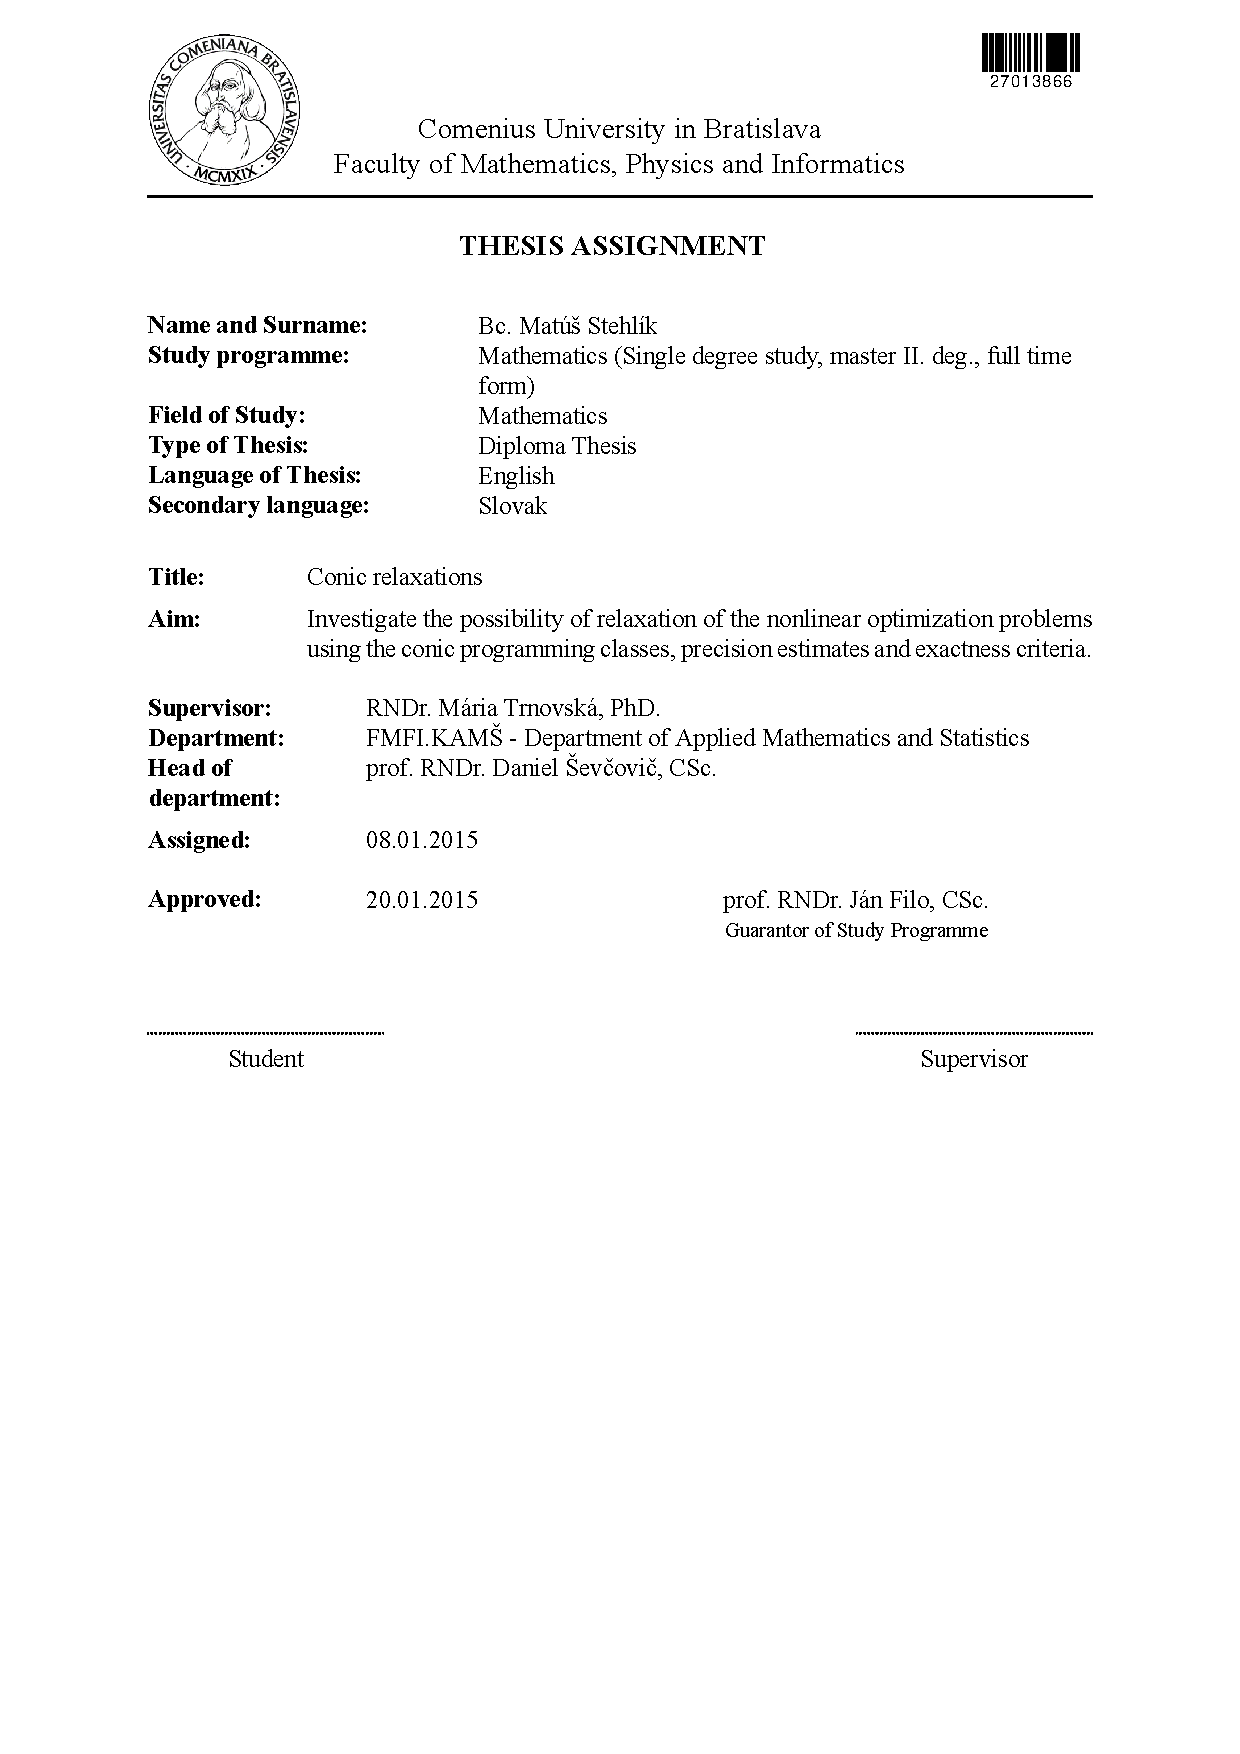
\includepdf{img/zadanie_en.pdf}




\eject % EOP ii

{~}\vspace{12cm}

\noindent
%\begin{minipage}{0.25\textwidth}~\end{minipage}
\begin{minipage}{1\textwidth}
{\bf Čestné vyhlásenie} \\
Vyhlasujem, že som túto diplomovú prácu vypracoval samostatne, pod vedením vedúceho práce a uviedol som všetku použitú odbornú literatúru.\\

\medskip

V Bratislave dňa 4. 5. 2016

\bigskip\bigskip

\hfill\hbox to 3.4cm{\dotfill} \\
\medskip
\hfill{Bc. Matúš Stehlík}\\ 
\end{minipage}
\vfill\null\eject % EOP iii
%~\vfill\eject % EOP iv

{\large\bf Poďakovanie}

\medskip

Ďakujem vedúcej tejto diplomovej práce RNDr. Márii Trnovskej PhD. za jej cenné rady, postrehy, odborné vedenie a pomoc počas vypracovávania práce.

\vfill\null\eject


{\large\bf Abstrakt}

\medskip

STEHLÍK, Matúš: {\it Kónické relaxácie}. Diplomová práca. Univerzita Komenského v Bratislave, Fakulta matematiky, fyziky a informatiky, Katedra matematickej analýzy a numerickej matematiky. Školiteľ: RNDr. Mária Trnovská PhD., Bratislava, 2016, 80 strán.

\bigskip

%\hspace*{1 cm} 
Diplomová práca sa venuje možnostiam relaxácie nekonvexných kvadratických optimalizačných úloh pomocou tried kónického programovania. Práca ponúka prehľad metód pre vytváranie kónických relaxácii. Podrobne sa venuje ich aplikácii na problém maximálneho rezu v grafe a porovnaniu ich efektivity na pri riešení tohto problému.


%Prvá kapitola uvádza triedy kónického programovania a vzťahy medzi nimi. V druhej kapitole sú zhrnuté metódy relaxovania pomocou uvedených tried. Tretia kapitola rozoberá aplikácie relaxačných techník na problém maximálneho rezu, kotré sú porovnané pomocou numerických experimentov v štvrtej kapitole. Dodatok uvádza základy teórie kužeľov a na príkladoch ukazuje vlastnosti kužeľov používaných v práci.


\bigskip

{\bf Kľúčové slová: }relaxácia, kužeľ, kónické programovanie, optimalizácia, se\-mi\-de\-fi\-ni\-tné programovanie, platé nerovnosti, problém maximálneho rezu \\

\newpage

{\large\bf Abstract}

\medskip

STEHLÍK, Matúš: {\it Conic relaxations}. Master thesis. Comenius University in Bratislava, Faculty of mathematics, physics and informatics, Department of mathematical analysis and numerical mathematics. Advisor:  RNDr. Mária Trnovská PhD., Bratislava, 2016, 80 pages.

\bigskip
This master's thesis explores the possibility of relaxation of the nonlinear quadratic
optimization problems using the conic programming classes. The thesis offers a
survey of techniques used for constructing conic relaxations.
The aforementioned techniques are applied to the max-cut problem and their performance on several different  instances of this problem is compared.

%
%First chapter introduces conic optimization classes and the relations between them. Second chapter surveys the methods of relaxation with conic programs. Third chapter analyses application of the relaxation techniques to the maximum cut probem, which are numerically compared in the fourth chapter. The appendix covers basic theory of cones with examples showing the properties of the cones used throughout the thesis. 


\bigskip

{\bf Key words: } relaxation, cone, conic programming, optimization, semidefinite programming, valid inequalities, maximum cut problem

\vfill\null\eject

\begin{spacing}{0.95}
\tableofcontents
\listoffigures
\begingroup
\let\clearpage\relax
\listoftables
\endgroup
\end{spacing}

\mainmatter

\chapter*{Introduction}
\addcontentsline{toc}{chapter}{Introduction}
\markboth{INTRODUCTION}{}

%%% problem statement
In this thesis we will study relaxation techniques for the quadratically constrained quadratic programs (QCQP).
\defi 
\label{defQCQP}
The Quadratically Constrained Quadratic Program (QCQP) in the standard form is
\begin{equation}
\label{qcqp} 
\begin{array}{ll}
\mbox{minimize}& x^TP_0x + q_0^Tx +r_0 \\
\mbox{subject to}& x^TP_kx + q_k^Tx + r_k \leq 0, \  (k = 1,\dots ,m),
\end{array} 
\end{equation}
where $x\in \mathbb{R}^n$ is a variable, and symmetric $n\times n$ matrices $P_0, P_1, \dots ,P_m \in S^n$, vectors $q_0,\dots ,q_m \in \mathbb{R}^n$ and scalars $r_1,\dots ,r_m\in \mathbb{R}$ are given.

%%%%% hardness
%The matrices $P_0, P_1, \dots P_m$ are not necessarily positive semidefinite. Therefore the objective function as well as the constraints may be nonconvex. Problem (\ref{qcqp}) has been proved to be NP-hard in general [\ref{PardalosQPisNPHard}], while several special subclasses
%of QCQP have been identified to be polynomially solvable (see [\ref{KimKojimaExactSolViaSDPandSOCP}]).
%
%%%% problems included
%For example, the 0-1 constraint $x_i\in \{0,1\}$ can be reformulated as $x^Te_ie_i^Tx - e_i^Tx =0$. Thus QCQP includes 0-1 programming, which describes various NP-hard problems, such as knapsack, stable set, maximum cut, quadratic assignment problem,  etc. 
%%Similarly. $\{-1,1\}$ constrained programming, which contains graph partitioning problems.
%On the other hand, the above examples suggest that QCQP has many applications and is worth solving.

%% hardness
In the QCQP the objective function as well as the constraints may be nonconvex. The problem has been proved to be NP-hard in general [\ref{PardalosQPisNPHard}], while several special subclasses
of QCQP have been identified to be polynomially solvable (see [\ref{KimKojimaExactSolViaSDPandSOCP}]).

However, the QCQP represents many problems with applications. For instance it includes 0-1 programming, which describes various NP-hard problems, such as knapsack, stable set, maximum cut, quadratic assignment problem,  etc. Therefore QCQP is worth solving, or rather approximating since it is computationally intractable.

% relaxation approach
One of the possible approaches is relaxing QCQP with convex problems which can be solved in polynomial time, namely linear programming (LP) [\ref{MargotLPRelax}], second order cone programming  (SOCP) [\ref{KimKojimaSOCPofNoncvxQOP}], or semidefinite programming (SDP) [\ref{HandbookSDP}].


% relaxation provides bounds
Since the relaxed problems are not equivalent to the original problem, solving them usually does not provide an exact solution. However, it gives a bound for optimal value. More specifically, in minimization problems, the optimal value of relaxation is a lower bound on the optimal value of the original problem. 

There are also methods (e.g. a projection or rounding procedures) to extract a feasible solution of the original problem from the optimum of relaxation. The feasible solution provides the opposite - the upper bound.


% approximation bounds
The quality of bounds depends widely on the problem and method of relaxation. For some problems the approximation ratio for certain relaxation is guaranteed. A widely known example is the SDP relaxation for the maximum cut by Goemans and WIlliamson [\ref{GoemansWilliamsonMaxCut}], which has guaranteed 0.878 approximation bound.

On the other hand, for many combinatorial problems there are also known certain inapproximability bounds which cannot be guaranteed for any polynomial approximation algorithm unless P is NP [\ref{Inapproximability results}]. 


% Branch and Bound
Bounds on the optimal value can be used to find the optimal solution with a proof of optimality. Such proof can be done e.g. by the so-called branch and bound (BnB) method, which is based on recursive subdividing of the feasible region into multiple segments and computing bounds on each of them separately. Whenever a bound for a segment is worse than the best known feasible solution, the segment is ruled out from consideration, because it was proven that it does not contain the optimal solution. 

The BnB method is usually used in combinatorial optimization, where the variables are discrete [\ref{ComparativeBNBStudyForGP}], however, it can be also adapted for nonconvex continuous optimization when the feasible region is compact [\ref{LinderothSimplicialBranchAndBound}, \ref{RaberSimplicialBranchAndBound}].

%%%%%% time-quality trade off
In practice, an important factor is time complexity, hence a relaxation giving the tightest bounds is not always a method of choice. Especially when using the BnB framework, where a sequence of relaxations needs to be solved [\ref{ComparativeBNBStudyForGP}].

Generally, SDP relaxation is supposed to produce stronger bounds then SOCP or LP relaxations, because those are subclasses of semidefinite programming. On the other hand, for the same reason, SOCP and LP relaxations should be easier to solve, therefore shorter computation time is expected advantage of these approaches. In fact, there is a certain speed versus quality "trade-off". 
An interesting method was proposed by Burer, Kim and Kojima [\ref{BurerKimKojimaFasterWeakerRelax}] for producing a relaxation "in-between" SDP and SOCP. 


%%%% Valid inequalities
It is known that the quality of relaxation also depends on the particular formulation of the problem. Adding redundant constraints to the problem may result in new constraints, called valid inequalities, tightening the relaxation [\ref{ZhengDCdecomp}, \ref{InexactSDPandValidIneq}, \ref{onValidIneqforQP}]. A popular method used for creating valid inequalities is the reformulation linearization technique (RLT) [\ref{AnstreicherSDPvsRLT}, \ref{SheraliAdamsRLT1}, \ref{SheraliEnhancingRLT}], which is based on multiplying pairs of linear constraints. In fact, Anstreicher [\ref{AnstreicherSDPvsRLT}] has shown that adding RLT constraints improves the SDP relaxation.

%%% hierarchies
Instead of following the heuristic approach of finding valid inequalities that may be helpful
for strengthening an LP or SDP, there is a more systematic (and potentially more powerful) approach
lying in the use of LP or SDP hierarchies. The idea is constructing a sequence of relaxations, each one providing better approximation of the problem, for the price of increasing dimension of the relaxed problem.
In particular there are procedures
by Balas, Ceria, Cornuéjols [\ref{BalasLiftandProjectCuttingPlane}], Lovász, Schrijver [\ref{LovaszSchriverHrierarchy}],  Sherali, Adams [\ref{SheraliAdamsHierarchy}] or Lasserre [\ref{LasserreExplicitExactSDP}, \ref{LasserreProblemOfMoments}]. The latter one was shown to be superior in the comparison by Laurent [\ref{LaurentComparisonOfHierarchies}].



%%%%% CP and CCP and DNN 
In 	2009, completely positive programming (CPP) relaxation for a class of binary quadratic problems was proposed
by Burer [\ref{BurerCPPreprOfBinLCQP}]. 
The class was extended to a more general class of QOPs by Eichfelder and
Povh [\ref{EichfelderPovhSetSDPreprOfQCQP}] and by Arima, Kim and Kojima [\ref{ArimaKimKojimaQCQPforCPP}]. Theoretically strong results were presented in
their papers [\ref{ArimaKimKojimaQCQPforCPP}, \ref{BurerCPPreprOfBinLCQP}, \ref{EichfelderPovhSetSDPreprOfQCQP}] showing that the exact optimal values of QOPs in their classes coincide
with the optimal values of their CPP relaxation problems.

Despite the CCP programs are convex, they are computationally intractable. On the other hand equivalent CPP formulations offer new insights which can lead to improvements of relaxation methods. 

A natural way of relaxing CPP is by doubly nonnegative program (DNN).
However, solving a DNN relaxation using a standard SDP solver is computationally costly compared to SDP relaxation due to the high number of linear (nonnegative) constraints. In [\ref{KimKojimaLagrangianDNNRelaxation1}] authors Kim, Kojima and Toh developed a technique to obtain Lagrangian DNN relaxation primal-dual pair, with single variable in the dual. Furthermore, they proposed a fast algorithm for solving their relaxation based on combination of bisection method and first order methods. Recently (February 2016), Arima, Kim, Kojima and Toh [\ref{ArimaKimKojimaRobustLagrangianDNN}] designed an improvement of the algorithm which achieves better robustness and acceleration. %Their approach has been shown to provide tight bounds for combinatorial problems as binary QPs, multiple knapsack problems, maximal stable set problems and the quadratic assignment problems.

\bigskip
%% in this thesis
In this thesis we will examine techniques for creating convex relaxations which can be applied to general QCQP or to some nonconvex subclass of QCQP such as binary quadratic programs. 

In the first chapter we will introduce convex optimization classes (LP, SOCP, SDP, CP and CCP) and relations between them. To conclude this chapter we will present a general conic programming class which includes all of previously mentioned programs as a special case. 

The second chapter will describe relaxation techniques. In the beginning we will propose our own definition to formally capture what is considered as relaxation in this thesis (not exclusively). Next we will discuss options for relaxing the nonconvex QCQP with problems in all conic classes mentioned in the first chapter, including the approaches for construction of valid inequalities. In the end of the chapter we will present a relaxation hierarchy by Lasserre.

The third chapter we will explore the maximum cut problem. As a motivation, we will present the famous result by Goemans and Williamson giving the 0.878 approximation guarantee for SDP relaxation. Next we will apply most of the relaxation methods from chapter 2, to formulate relaxations of max-cut. The relaxations will also include triangle inequalities - the problem specific valid inequalities for max-cut.

In the last chapter we will computationally compare the relaxation methods for the max-cut stated in the chapter 3.  We will perform numerical experiments comparing the performance of relaxations on max-cut instances of various size and sparsity. Next we will describe branch and bound framework and use it to compare the performance of chosen methods in this procedure.


In the appendix we will cover basic properties of cones and include examples showing the important properties of the cones used throughout the thesis. 




\newpage
\section*{Notation}
%TODO hlavicka Notation , to Contents
\addcontentsline{toc}{section}{Notation}
\markboth{INTRODUCTION}{NOTATION}


\subsubsection{Sets}
\begin{tabular}{lcl}
$\mathbb{R}$ &-& Set of real numbers \\
$\mathbb{R}_+$ &-& Set of non-negative real numbers \\
$\mathbb{R}^n$ &-& Set of $n$-dimensional real vectors   \\
$\mathbb{R}^n_{+}$ &-&  Set of $n$-dimensional real vectors with non-negative entries  \\

$S^n$ &-& Unit sphere in $\mathbb{R}^n$ \\

$\mathbb{Q}^n$ &-& Second order cone \\

$\mathbb{S}^n$ &-& Set of symmetric $n\times n$ matrices \\
$\mathbb{S}^n_+$ &-& Set of symmetric $n\times n$ positive semidefinite  matrices \\& & (positive semidefinite cone) \\
$\mathbb{S}^n_{++}$ &-& Set of symmetric positive definite $n\times n$ matrices \\

$\mathbb{C}^n$ &-& Set of symmetric copositive $n\times n$ matrices (copositive cone) \\
$\mathbb{P}^n$ &-& Set of symmetric completely positive $n\times n$ matrices \\& & (completely positive cone)\\
$\mathbb{N}^n$ &-& Set of symmetric nonnegative $n\times n$ matrices (nonnegative cone) \\
$\mathbb{S}^n_+ \cap \mathbb{N}^n$ &-& Doubly nonnegative cone (DNN) \\
$\Gamma $ &-& Set of positive rank 1 matrices\\
\end{tabular}

\subsubsection{Operators}
\begin{tabular}{lcl}
$M\succ 0$ &-& M is symmetric and positive definite \\
$M\succeq 0$ &-& M is symmetric and positive semidefinite \\
$M_1 \succeq M_2$ &-& $M_1 - M2\succeq 0$ \\
$C\bullet X$ &-& Matrix inner product $=Tr(C^TX)$ \\

$conv(K)$ &-& Convex hull of $K$ \\
$svec(\cdot)$ &-& An operator transforming a symmetric $n\times n$  matrix into a vector \\& &  of its entries in $\mathbb{R}^{n(n+1)/2}$ \\
$(x;y)$ &-& Column vector $(x^T,y^T)^T$
\end{tabular}

\subsubsection{Abbreviations}
\begin{tabular}{lcl}

PSD &-& Positive Semidefinite \\

QCQP &-& Quadratically Constrained Quadratic Program \\
CQP &-& Convex Quadratic Program (a convex QCQP) \\
LP &-& Linear Program \\
SOCP &-& Second Order Cone Program \\
SDP &-& Semidefinite program \\
CP &-& Copositive program \\
CPP &-& Completely positive program \\
& & \\ 
%BnB &-& Branch and Bound 	
\end{tabular}





\chapter{Conic optimization classes}
\label{ConicOptClasses}

In this section we will introduce basic optimization classes mentioned above, in particular  linear programming (LP), second order cone programming  (SOCP), or semidefinite programming (SDP). We will state the problems in standard forms and their duals. The dual problems will be only mentioned here and will be derived in the next section. We will also show that LP is subclass of convex QCQP, convex QCQP is subclass of SOCP, and SOCP is subclass of SDP, i.e.
\begin{equation*}
LP\subset CQP \subset SOCP \subset SDP. %\subset QCQP 
\end{equation*}

As a sources for this chapter we refer to [\ref{BoydCvxOpt},\ref{IntroToCvxOptBerkley}] as general sources and specifically to SOCP [\ref{KimKojimaSOCPofNoncvxQOP}, \ref{GoldfarbSOCP}, \ref{PokornaSOCPDipl}], SDP [\ref{HandbookSDP}, \ref{KimKojimaSOCPofNoncvxQOP}], CP and CPP [\ref{ArimaKimKojimaQCQPforCPP}, \ref{BurerCPPreprOfBinLCQP}, \ref{DurCopositiveSurvey}].












\section{Linear programming}

When both, the objective and the constraint functions are linear (affine), the problem is called a linear program and it belongs to the Linear Programming class, or shortly LP.
In this section we will introduce the standard form of LP and its dual. For reference and more information about this topic see i.e. [\ref{BoydCvxOpt}] .

\defi
\label{defLP}
The primal--dual pair of linear programs in standard form is 
\begin{equation}
\label{LP} 
\begin{array}{cc}
Primal & Dual \\
% \hline \\
\begin{array}{ll}
\mbox{minimize} & c^Tx, \\
\mbox{subject to}& Ax = b ,  \\
& x \in \mathbb{R}^n_+,\\

\end{array} 
\ \ \ \ \ & \ \ \ \ \ 
\begin{array}{ll}
\mbox{maximize} & b^Ty, \\
\mbox{subject to}& A^Ty +s = c ,  \\
& s\in \mathbb{R}^n_+, \\
\end{array}
\end{array} 
\end{equation}
where $x\in R^n$, $y\in \mathbb{R}^m$ , $s\in \mathbb{R}^n$ are the variables; the real $m\times n$ matrix $A$ and vectors $b \in \mathbb{R}^m, c\in \mathbb{R}^n$ are given problem data.

\bigskip

\rem Linear programs can be formulated in various forms (including $\geq , \leq$ inequalities, free variables, possibly some linear fractions in objective) but all of them can be transformed to the standard form.
%
%\subsection{Relation to previous classes}
%Linear programming is a special case of QCQP, when all matrices in quadratic forms are 0.


\section{Second order cone programing}
\label{SectionSOCP}


The second order cone programming (SOCP) is a convex optimization class, which can be solved with great efficiency using interior point methods. 
In this section we will introduce the standard form of SOCP and its dual. For reference and more information about this topic see [\ref{BoydCvxOpt}] .


Let us first define second order cone.
\defi[Second order cone]
\label{defSOC} We say $\mathbb{Q}^n$ is second order cone of dimension $n$ if 
\begin{equation*}
\mathbb{Q}^n=\{x\in \mathbb{R}^n \ | \ x = (x_0;\bar{x}) \in \mathbb{R}\times\mathbb{R}^{n-1}, \|\bar{x}\|_2\leq x_0\}.
\end{equation*}


\defi[SOCP]
\label{defSOCP}
The primal--dual pair of the Second Order Cone Program (SOCP) in the standard form is
\begin{equation}
\label{socp} 
\begin{array}{cc}
Primal & Dual \\
%\hline \\
\ \ \ \begin{array}{ll}
\mbox{minimize} & c^Tx,\\
\mbox{subject to}& Ax = b,\\
& x \in \mathbb{Q}^n,
\end{array} 
 \ \ \ \ \ & \ \ \ \ \ 
 \begin{array}{ll}
\mbox{maximize} & b^Ty,\\
\mbox{subject to}& A^Ty + s = c,\\
& s \in \mathbb{Q}^n,
\end{array}
\end{array}
\end{equation}
where $x\in \mathbb{R}^n$ , $y\in \mathbb{R}^m$ and $s\in \mathbb{R}^n$ are the variables; and $m\times n$ real matrix $A$, vectors $c\in \mathbb{R}^n$, $b\in \mathbb{R}^{m},$ $c\in \mathbb{R}^n$ are given problem data.

\rem Second order cone programs can be formulated in various forms (including quadratic objective or several second order cone constraints of the affine functions), but all of them can be transformed to the standard form. 

\rem In general, any program of the form 
\begin{equation}
\begin{array}{cc}
Primal & Dual \\
%\hline \\
\begin{array}{ll}
\mbox{min} &  c^{1T}x^1+\cdots + c^{kT}x^k,\\
\mbox{s.t.}& A^1x^1+ \cdots + A^kx^k = b, \\
& x^i \in \mathbb{Q}^{n_i}, \ (i = 1,\dots ,k),
\end{array} 
 & 
 \begin{array}{ll}
\mbox{max} & b^Ty,\\
\mbox{s.t.}& A^{iT}y + s^i = c^i, \\ %\ (i = 1,\dots ,k)
& s^i \in \mathbb{Q}^{n_i}, \ (i = 1,\dots ,k),
\end{array}
\end{array}
\label{genSOCP}
\end{equation}
is considered to be SOCP.
The second order cone constraints can be also formulated as, $x = (x^1,\dots ,x^k) \in \mathbb{Q},$ where $\mathbb{Q}$ is Cartesian product of second order cones, 
\begin{equation}
\mathbb{Q} = \mathbb{Q}^{n_1}\times \mathbb{Q}^{n_2}\times \cdots \times \mathbb{Q}^{n_k},
\end{equation}
 such $\mathbb{Q}$ has all important properties of second order cone, 
and algorithmic aspects of solving standard SOCP can also be applied for this more general case [\ref{GoldfarbSOCP},\ref{PokornaSOCPDipl}].
In order to keep things simple, we will sometimes consider only the standard form stated in the Definition \ref{defSOCP}, but all the details can be also done for this more general form.


\subsection{Relation to previous classes}
\label{SectionRelBtwSOCPandQCQP}

Second Order Cone Programming includes convex LP as special case.
We will show that SOCP in fact includes CQP as a subclass. We will demonstrate procedure proposed in [\ref{KimKojimaSOCPofNoncvxQOP}] used to reformulate CQP as SOCP.

Let us have a CQP. In other words, suppose that $n\times n$ matrices $P_k$, $k=0,\dots ,m$ are positive semidefinite. 
\begin{equation*}
\begin{array}{ll}
\mbox{minimize}& x^TP_0x + q_0^Tx + r_0, \\
\mbox{subject to}& x^TP_kx + q_k^Tx + r_k \leq 0, \  (k = 1,\dots ,m),
\end{array} 
\end{equation*}
First of all, rewrite problem equivalently as
\begin{equation*}
\begin{array}{ll}
\mbox{minimize}& t, \\
\mbox{subject to} & x^TP_0x + q_0^Tx + r_0 \leq t,\\
& x^TP_kx + q_k^Tx + r_k \leq 0, \  (k = 1,\dots ,m).
\end{array} 
\end{equation*}

To avoid tedious notation, without loss of generality, suppose that considered program already has linear objective function (i.e. $P_0 = 0$).  Also suppose that we have separated all the linear constraints (ones where $P_k = 0$) and arrange them into more compact form $Ax=b$. Even if we did not, the following procedure will still be correct, but will result in more complicated formulation of linear constraints.

Each convex quadratic constraint 
\begin{equation}
\label{QuadConstraint}
x^TPx + q^Tx + r \leq 0
\end{equation} 
can be transformed into the second order cone constraint.  Suppose that $P\neq 0$ and rank $P = h.$ Then there exists $n\times h$ matrix $L$ such that $P=LL^T$. Such $L$ can be computed by Choelsky factorization of $P$. Now rewrite (\ref{QuadConstraint}) as 
\begin{equation}
\label{ConvertToSOCP1}
(L^Tx)^T(L^Tx)\leq -q^Tx - r.
\end{equation}
It can be easily verified that $w\in \mathbb{R}^t$, $\xi \in \mathbb{R}$ and $\eta \in \mathbb{R}$ satisfy
$$w^Tw\leq \xi\eta, \ \ \xi\geq 0\ \mbox{ and } \ \eta\geq 0$$
if and only if they satisfy
$$\left\|\left( \begin{array}{c}
\xi-\eta\\
2w
\end{array}\right)\right\|_2
\leq \xi+\eta . $$
If we take $w=L^Tx, \ \xi = 1$ and $\eta = -q^Tx - r$, then inequality (\ref{ConvertToSOCP1}) is equivalent to the second order cone constraint
\begin{equation}
\label{ConvertedQCintoSOCC}
 \|v\|_2\leq v_0, \ \mbox{  where  } \ \left(\begin{array}{c}
v_0\\
v
\end{array}\right) = 
\left(\begin{array}{c}
1- q^Tx - r\\
1 + q^Tx + r\\
2L^Tx
\end{array}\right)\in \mathbb{R}^{h+2}.
\end{equation}

Now the intersection of all such second order cone constraints can be easily expressed as Cartesian product of second order cones, thus we have obtained problem of SOCP in form \ref{genSOCP}. 


\section{Semidefinite programming}




The semidefinite programming (SDP) is a convex optimization class which can be solved efficiently using interior point methods. In this section we will introduce the standard form of SDP and its dual. For reference and more information about this topic see [\ref{BoydCvxOpt}] .


Firstly, let us introduce notation we will use to simplify the standard form.

\defi 
\label{defBullet}
Let $A,X$ be real $n\times m$ matrices, we will denote their inner product 
$$A\bullet X = Tr(A^TX).$$
Where $Tr(M)$ denotes trace of matrix $M$ i.e. sum of the diagonal elements of $M$.

\defi[SDP]
\label{defSDP}
The primal--dual pair of the Semidefinite Program (SDP) in the standard form is
\begin{equation}
\label{sdp} 
\begin{array}{cc}
Primal & Dual \\
\begin{array}{ll}
\mbox{minimize} & A_0\bullet X,\\
\mbox{subject to}& A_k\bullet X  = b_k, \ \\
 & ( k = 1,\dots ,m), \\
& X \in \mathbb{S}^n_+,
\end{array}
\ \  &  \ \
\begin{array}{ll}
\mbox{maximize} & b^Ty, \\
\mbox{subject to}& \sum_{k=1}^m y_kA_k + S  = A_0 ,\\
& S \in \mathbb{S}^n_+,
\end{array}
\end{array}
\end{equation}

where $X\in \mathbb{S}^n_+$, $y = (y_1,\dots ,y_m)^T\in \mathbb{R}^m$ and $S\in \mathbb{S}^n$ are the variables; and symmetric matrices $A_0 , A_1,\dots , A_m \in \mathbb{S}^n$ and scalars $b_1,\dots, b_m \in \mathbb{R}$ are given.


Surprisingly, the variable in SDP is a symmetric matrix (not a vector). 
In order to be consistent with other classes we will sometimes use a $svec$ operator.  

\defi \label{svec}
We define operator $svec: \mathbb{S}^n \rightarrow \mathbb{R}^{n(n+1)/2}$, such that for any $n\times n$ symmetric matrix $M$
%\begin{equation*}
%svec(M) = (M_{11}, \frac{\sqrt{2}}{2}M_{12}, \dots, \frac{\sqrt{2}}{2}M_{1n}, M_{22}, \frac{\sqrt{2}}{2}M_{23}, \dots, \frac{\sqrt{2}}{2}M_{2n},  \dots, M_{nn})^T
%\end{equation*}
\begin{equation*}
	svec(M) = ( \delta_{11}M_{11},\delta_{12}M_{12},\delta_{22}M_{22},\dots ,\delta_{1n}M_{1n},\dots ,\delta_{nn}M_{nn})^T,
\end{equation*}
where
\begin{equation*}
	\delta_{ij}= \left\lbrace 
	\begin{array}{ll} 
		1, &\mbox{ if }\ i=j, \\ 
		\sqrt{2}, &\mbox{ otherwise.} 
	\end{array} \right.
\end{equation*}

Notice that $\delta_{ij}$ are defined cleverly, so that inner product of symmetric matrices is equivalent to the standard inner product of their images
\begin{equation*}
A\bullet X= svec(A)^Tsvec(X), 
\end{equation*}
for any pair of symmetric matrices $A,X\in \mathbb{S}^n.$  Now we can easily formulate the problems of SDP in terms of standard inner product over the space of real vectors. 
\begin{equation}
\label{svecSDP}
\begin{array}{ll}
\mbox{minimize} & svec(A_0)^T svec(X),\\
\mbox{subject to}& svec(A_k)^T svec(X)  = b_k, \ (k = 1,\dots ,m), \\
& svec(X) \in \mathcal{K}(\mathbb{S}^n_+),
\end{array}
\end{equation}
where $svec(X)$ is variable,  $\mathcal{K}(\mathbb{S}^n_+) = \{svec(U)\in \mathbb{R}^{n(n+1)/2}\ |\ U\in \mathbb{S}^n_+\}$ 
and problem data are from the standard SDP (\ref{sdp}).


\subsection{Relation to previous classes}
The  SDP primal-dual pair looks suspiciously similar to the both LP and SOCP primal-dual pairs. 
The only difference between LP and SOCP is the nonnegative orthant is replaced by second order cone. 
The SDP, in the $svec$-operator form (\ref{svecSDP}), further generalizes the cone constraint with the semidefinite cone.

In fact, SOCP is subclass of SDP. We will show how the standard SOCP can be rewritten as SDP.
First of all, instead of minimizing $c^Tx$ we will minimize $t$ with additional constraint $t\geq c^Tx$. 
%which we will add to other linear constraints as a new row in $A$ and $b$.

The only nontrivial part is to rewrite conic constraint 
\begin{eqnarray*}
& &x\in \mathbb{Q}^n \ \Leftrightarrow  \ ||\bar{x}||\leq x_1 \ \Leftrightarrow  
\left\lbrace \begin{array}{r}
\bar{x}^T\bar{x}\leq x_1^2\\
0\leq x_1 
\end{array}\right\rbrace \\
 & &\Leftrightarrow \ 
 \left\lbrace \begin{array}{r}
\frac{\bar{x}^T\bar{x}}{x_1}\leq x_1\\
0\leq x_1 
\end{array}\right\rbrace 
 \ \Leftrightarrow  \ 
 \left( \begin{array}{cc}
x_1 & \bar{x}^T\\
\bar{x} & x_1I_{n-1}
\end{array}\right)\succeq 0.
\label{arrowx}
\end{eqnarray*}
Where last equivalence is provided by Schur complement lemma (see appendix, Theorem \ref{SchurCompl}). The case when $x_1=0$ is trivial, one can see that as zero vector belongs to $\mathbb{Q}^n$ also zero matrix satisfies given semidefinite constraint. 
%TODO From here, it can be easy brought to the standard form (see appendix). 

%It can be rewritten as linear matrix inequality (LMI)
%\begin{equation}
%x_1I_n + \sum_{k=2}^n x_kE_{1k} \succeq 0
%\end{equation}
%The linear constraint $Ax = b$ can be easily cast to LMI form with
%%\begin{equation}
%% a_k^Tx = b_k \ \Leftrightarrow \ 
%% \left(\begin{array}{cc}
%% a_{k1}&\bar{a}_k^T/2\\
%% \bar{a}_k/2& 0
%% \end{array}\right)\bullet X = b_k,
%%\end{equation} 
%%where $a_k^T = (a_{k1}, \bar{a}_k^T)$ is the $k$-th row of $A$. 
%\begin{equation}
%Ax=b \ \Leftrightarrow \ diag(Ax-b,b-Ax)\succeq 0,
%\end{equation}
%where $diag(v)$ is the diagonal matrix with entries of $v$ on the main diagonal.
%The resulting 2 LMIs can be simply combined into single one as a block diagonal matrix. The resulting SDP is then
%\begin{equation} 
%\begin{array}{l}
%\mbox{maximize \ }  c^Tx \\
%\mbox{s.t. \ }
%% diag(0,Ax-b,b-Ax)+x_1diag(I_n,0,0) + \sum_{k=2}^n x_kdiag(E_{1k},0,0) \succeq 0.
% diag\left(\begin{array}{c} 0 \\ Ax-b \\b-Ax  \end{array}\right) 
% +  x_1diag\left(\begin{array}{c} I_n \\ 0 \\0  \end{array}\right)
% + \sum_{k=2}^n x_kdiag\left(\begin{array}{c} E_{1k} \\0 \\0  \end{array}\right)\succeq 0.
% \end{array}	
%\end{equation}  



In case of more general standard form of SOCP (\ref{genSOCP}), the $x\in \mathbb{Q}$ constraint 
can be transformed similarly. 
\begin{equation*}
x = (x^1,\dots, x^k)^T \Leftrightarrow  M = diag(M_1,\dots, M_k) \succeq 0,
\end{equation*}
where $M$ is a block diagonal matrix, with blocks $M_i$ of the form (\ref{arrowx}), for $i=1,\dots, k$,
corresponding to the constraints $x^i\in \mathbb{Q}^{n_i}$.



\section{Copositive and completely positive programming}


The copositive programming (CP) and completely positive programming (CPP) are convex conic classes which are %important mainly for theoretical interests since CCP and CP problems are 
numerically intractable. 
In fact, it is known that determining whether a matrix is copositive is co-NP-complete 	[\ref{MurtyNPcompleteQP}]. 
%Intuitively, checking that matrix is completely positive should have the same computational complexity. It seems, however, that a formal proof of this statement has not yet been given [\ref{DurCopositiveSurvey}].

However, these optimization classes seem to play an important role in current research. Recently, multiple classes of QCQP have been equivalently reformulated as convex completely positive or copositive programs [\ref{ArimaKimKojimaQCQPforCPP}, \ref{BurerCPPreprOfBinLCQP}, \ref{EichfelderPovhSetSDPreprOfQCQP}]. While restating of the problem as an optimization problem over one of these cones does not resolve
the difficulty of that problem, studying properties of $\mathbb{C}^n$ and $\mathbb{P}^n$ and
using the conic formulations of quadratic and combinatorial problems does
provide new insights and computational improvements. (see the survey of Copositive programming [\ref{DurCopositiveSurvey}])


Let us first define the copositive cone and completely positive cone.
\defi[Copositive cone]
\label{defCopositiveCone} We say $\mathbb{C}^n$ is copositive cone of dimension $n$ if 
\begin{equation*}
\mathbb{C}^n=\{M\in \mathbb{S}^n \ | \ x^TMx\geq 0 \ \forall x\in \mathbb{R}^n_+ \}.
\end{equation*}
A matrix $M \in \mathbb{C}^n$ is called copositive.


\defi[Completely positive cone]
\label{defCPPcone} We say $\mathbb{P}^n$ is completely positive cone of dimension $n$ if 
\begin{equation*}
\mathbb{P}^n=\{M\in \mathbb{S}^n \ | \ M = \sum_{i = 1}^l x^{i}x^{iT} \ \mbox{ where } x^i \in \mathbb{R}^n_+ \ (i = 1,\dots ,n) \}.
\end{equation*}
A matrix $M\in \mathbb{P}^n$ is called completely positive.

In fact, $\mathbb{C}^n$ and $\mathbb{P}^n$ are closed convex cones and they are dual cones to each other.
That is $\mathbb{P}^n$ is the dual cone of the $\mathbb{C}^n$ and vice versa (see Examples \ref{ExClosedConvexCones} , \ref{ExDualCones} in the Appendix).



\defi[]
\label{defCPandCPP}
The primal--dual pair of the copositive (CP) and the completely positive (CPP) program is
\begin{equation}
\label{cp&cpp} 
\begin{array}{cc}
Primal & Dual \\
\begin{array}{ll}
\mbox{minimize} & A_0\bullet X,\\
\mbox{subject to}& A_k\bullet X  = b_k, \ \\
 & ( k = 1,\dots ,m), \\
& X \in \mathbb{C}^n,
\end{array}
\ \  &  \ \
\begin{array}{ll}
\mbox{maximize} & b^Ty, \\
\mbox{subject to}& \sum_{k=1}^m y_kA_k + S  = A_0 ,\\
& S \in \mathbb{P}^n, \\
&
\end{array}
\end{array}
\end{equation}
where $X,\ S\in \mathbb{S}^n$ and $y\in \mathbb{R}^m$ are the variables;  matrices $A_0,\dots ,A_m\in \mathbb{S}^n$ and vector $b=(b_1,\dots ,b_m)^T\in \mathbb{R}^m$ are given problem data.

Similarly to SDP (\ref{svecSDP}), this problem can be reformulated using $svec(\cdot )$ operator to obtain the same form as all the previous classes with vector variable and standard inner product as an objective.
\subsection{Relation to previous classes}
In this section we will first describe the relations of $\mathbb{C}^n $ and $\mathbb{P}^n$ to the other cones. Then we will show that SDP is a subclass of CP, and in the end we will provide a simple example of the equivalent CPP reformulation for a special class of nonconvex QP.

\subsubsection{Relation to other cones}
First, let us define two other important cones
\defi[]
\label{defGammaAndNandDNNcones}
We will denote 
\begin{eqnarray*}
\Gamma &:=& \{ xx^T \ \vert \ x\in\mathbb{R}^n_+ \}  \ \mbox{ the cone of positive rank 1 matrices}, \\
\mathbb{N}^n &:=& \{ M\in \mathbb{S}^n \ \vert \ M_{ij} \geq 0, \forall \ 1\leq i,j\leq n \} \ \mbox{ the nonnegative cone}.
\end{eqnarray*}
and say a matrix $M\in \mathbb{N}^n$ is nonnegative. Especially, when $M \in \mathbb{S}^n \cap \mathbb{N}^n$ then we call $M$ a doubly nonnegative matrix, and we will refer to $\mathbb{S}^n \cap \mathbb{N}^n$ as doubly nonnegative cone.






\lema
\label{lemmaCPPSDPCP} It holds that  
$\ \mathbb{P}^n \subset \mathbb{S}^n_+ \subset \mathbb{C}^n. $ \rm
\begin{proof}
For a completely positive matrix $M=\sum_i x^i(x^i)^T$ with $x^i \in \mathbb{R}^n_+$ and an arbitrary vector $y\in\mathbb{R}^n_+$ it holds that 
$$ y^TMy = \sum_i y^Tx^i(x^i)^Ty = \sum_i (y^Tx^i)^2 \geq 0.$$
Therefore $M$ is positive semidefinite and since this is true for any $M\in \mathbb{P}^n$ we have the first inclusion $\mathbb{P}^n \subset \mathbb{S}^n_+$.

A positive semidefinite matrix $M\in\mathbb{S}^n_+$ suffices $x^TMx\geq 0$ for all $x\in \mathbb{R}^n$, therefore also 
for all $x\in \mathbb{R}^n_+$. Hence $ \mathbb{S}^n_+ \subset \mathbb{C}^n. $
\end{proof}

A following proposition states the relations between positive semidefinite, copositive and completely positive matrices.

\prop It holds that 
\label{ConesInclusionsProp}
$$\Gamma \ \subset \ \mathbb{P}^n \ \subset \ \mathbb{S}^n_+ \cap \mathbb{N}^n \ \subset \ \mathbb{S}^n_+ \ \subset \ \mathbb{S}^n_+ + \mathbb{N}^n \ \subset \ \mathbb{C}^n. $$ \rm

\rem For $n\leq 4$ it hods that $\mathbb{P}^n = \mathbb{S}^n_+ \cap \mathbb{N}^n$ and $\mathbb{S}^n_+ + \mathbb{N}^n = \mathbb{C}^n.$

\begin{proof}[Proof of Proposition \ref{ConesInclusionsProp}]
We will proceed through inclusions from left to right. The first inclusion $\Gamma\subset \mathbb{P}^n$ is trivial. It is also easy to see that all matrices in $\mathbb{P}^n$ are nonnegative, therefore $\mathbb{P}^n \subset \mathbb{N}^n$. Together with $\mathbb{P}^n \subset \mathbb{S}_+^n$ from th lemma we have $\mathbb{P}^n \subset \mathbb{S}^n \cap \mathbb{N}^n$. The assertions $\mathbb{S}^n \cap \mathbb{N}^n \subset \mathbb{S}^n \subset \mathbb{S}^n + \mathbb{N}^n$ are trivial. Now we only need to prove that $\mathbb{S}^n + \mathbb{N}^n\subset \mathbb{C}^n. $ But this is an easy exercise since $\mathbb{C}^n$ contains both $\mathbb{S}^n$ and $\mathbb{N}^n$ (former by lemma, latter trivially), and $\mathbb{C}^n$ is convex (see Example \ref{ExClosedConvexCones} in the Appendix).
\end{proof}




\subsubsection{Relation to SDP}
To establish that SDP is a subclass of copositive programming we only need to reformulate the semidefinite constraint $X\succeq 0$ in terms of linear and copositive cone constraints.

Every vector $v\in \mathbb{R}^n$ can be written as difference of two positive vectors 
$v = x-y$, $x,y\in\mathbb{R}^n_+$. Therefore a symmetric matrix $X\in\mathbb{S}^n$ is positive semidefinite if and only if 
$$(x-y)^TX(x-y)  \geq 0, \ \ \forall x,y\in\mathbb{R}^n_+$$
This condition can be rewritten as 
$$u^TCu \geq 0, \ \forall u\in\mathbb{R}^n_+, \ \mbox{ where } \ 
u = \left(\begin{array}{c} x \\ y \end{array}\right), \ \mbox{ and } \
C = \left(\begin{array}{rr} X & -X \\ -X & X \end{array}\right).
$$
Which is equivalent to $C\in\mathbb{C}^{2n}$. Also it is clear that this form of $C$ can be enforced with linear equalities, therefore semidefinite programming is indeed a subclass of copositive programming.

\subsubsection{Relation to QP}

In 	2009, completely positive programming (CPP) relaxation for a class of binary QOPs was proposed
by Burer [\ref{BurerCPPreprOfBinLCQP}]. 
The class was extended to a more general class of QOPs by Eichfelder and
Povh [\ref{EichfelderPovhSetSDPreprOfQCQP}] and by Arima, Kim and Kojima [\ref{ArimaKimKojimaQCQPforCPP}]. Theoretically strong results were presented in
their papers [\ref{ArimaKimKojimaQCQPforCPP}, \ref{BurerCPPreprOfBinLCQP}, \ref{EichfelderPovhSetSDPreprOfQCQP}]


Copositive programming is closely related to quadratic and combinatorial
optimization. 
We illustrate this connection by means of the standard quadratic
problem (an example from [\ref{DurCopositiveSurvey}]).
\begin{equation}
\label{SimpleQP1}
\begin{array}{ll}
\mbox{minimize} & x^TQx,\\
\mbox{subject to}& e^Tx   = 1, \ \\
& x \in \mathbb{R}^n_+,
\end{array}
\end{equation}
where $e$ denotes the all ones vector. Rewriting the objective $x^TQx = Q\bullet xx^T$ and linear constraint $e^Tx = 1 $ as $ee^T\bullet xx^T = 1$, one can see that  
\begin{equation}
\label{SimpleQP1 CCP relax}
\begin{array}{ll}
\mbox{minimize} & Q\bullet X,\\
\mbox{subject to}& ee^T\bullet X  =1 , \\
& X \in \mathbb{P}^n,
\end{array}
\end{equation}
is a relaxation of (\ref{SimpleQP1}). Since the objective is now linear, an
optimal solution must be attained in an extremal point of the convex feasible
set. It can be shown that these extremal points are exactly the positive rank 1
matrices $xx^T$ with $x\in\mathbb{R}^n_+$ and $e^T x = 1$ (see the Lemma \ref{convHullReprLema} bellow). Together, these results imply that (\ref{SimpleQP1 CCP relax}) is in fact an exact reformulation of (\ref{SimpleQP1}).

\lema \label{convHullReprLema} It holds that $$\{X\in \mathbb{P}^n\ \vert \ ee^T\bullet X = 1\} = conv\left( \{ xx^T \ \vert \ x\in\mathbb{R}^n_+, \ e^T x = 1 \}\right). $$ \rm
\begin{proof}
Let $X\in\mathbb{P}^n$ satisfy $ee^T\bullet X = 1$. We will show that $X$ can be written as convex combination of vectors from $\Gamma_1:= \{ xx^T \ \vert \ x\in\mathbb{R}^n_+, \ e^T x = 1 \}.$ 

From the definition of $\mathbb{P}^n$, there are $x^1,\dots ,x^l\in \mathbb{R}^n_+$, such that  
\begin{equation*}
 X  \sum_{i=1}^l x^i(x^i)^T = \sum_{i=1}^l  (e^Tx^i)^2 \left(\frac{x^i}{e^Tx^i}\right)\left(\frac{x^i}{e^Tx^i}\right)^T =  \sum_{i=1}^l  \alpha_i y^i(y^i)^T
\end{equation*}
where $\alpha_i = (e^Tx^i)^2$ and $y^i =  x^i/(e^Tx^i)$. It is easy to see that $y^i\in \mathbb{R}^n_+$ and $e^Ty^i = 1$, so $y^i(y^i)^T\in \Gamma_1$.  
Also, it holds that $\sum \alpha_i = 1$, since 
\begin{equation*}
1 = ee^T\bullet X = ee^T\bullet \sum_{i=1}^l x^i(x^i)^T = \sum_{i=1}^lee^T\bullet x^i(x^i)^T = \sum_{i=1}^l (e^Tx^i)^2 = \sum_{i=1}^l \alpha_i.
\end{equation*}
Therefore $X = \sum_{i=1}^l  \alpha_i y^i(y^i)^T$ is a convex combination of vectors from $\Gamma_1$, hence $X\in conv(\Gamma_1)$.

We have shown that $\{X\in \mathbb{P}^n\ \vert \ ee^T\bullet X = 1\} \subseteq conv(\Gamma)$. Since the other inclusion is obvious, the proof is complete.

\end{proof}


%TODO CCP reformulation of SDP dual?


\section{General conic programming approach}

All of the previously mentioned classes are quite similar. 
With respect to their variable space, all of them have linear objective, linear constraints and cone constraint.

In fact, they are special cases of the so-called conic linear programs.




%Now we can define conic program which generalizes all previous classes.
\defi[Conic Programming] 
\label{defConeProg}
The primal--dual pair of the Linear Conic Program in the standard form is  
\begin{equation}
\label{coneProg} 
\begin{array}{cc}
Primal & Dual \\
\ \ \ \begin{array}{ll}
\mbox{minimize} & c^Tx,\\
\mbox{subject to}& Ax = b,\\
& x \in \mathcal{K},
\end{array} 
 \ \ \ \ \ & \ \ \ \ \ 
 \begin{array}{ll}
\mbox{maximize} & b^Ty,\\
\mbox{subject to}& A^Ty + s = c,\\
& s \in \mathcal{K}^*,
\end{array}
\end{array}
\tag{Conic Program}
\end{equation}
where $x\in \mathbb{R}^n$ , $y\in \mathbb{R}^m$ and $s\in \mathbb{R}^n$ are the variables; and $m\times n$ real matrix $A$, vectors $c\in \mathbb{R}^n$, $b\in \mathbb{R}^{m},$ $c\in \mathbb{R}^n$, and the proper cone $\mathcal{K}$ are given problem data. 

\rem
We say $\mathcal{K}$ is a proper cone if it is a cone and is closed, convex, pointed and has nonempty interior (see the Definition \ref{defProperCone} and the Example \ref{ExProperCones} in the Appendix). The 
\begin{equation*}
{K}^* = \{z\ |\ \forall x\in\mathcal{K}, \ x^Tz\geq 0\},
\end{equation*} 
denotes the dual cone of $\mathcal{K}$ (see the Example \ref{ExDualCones} in the Appendix).

Conic programming contains, but is not limited to, any problems combined from LP, SOCP and SDP programs. 
For example 
\begin{equation*}
\begin{array}{ll}
\mbox{minimize} & c^Tx,\\
\mbox{subject to}&A^ix^i=b^i, \ (i = 1,\dots ,k),\\
& x=(x^1,\dots ,x^k) \in \mathcal{K} = (\mathcal{K}^1,\dots ,\mathcal{K}^k),
\end{array} 
\end{equation*}
where the variable $x=(x^1, \dots, x^k)^T$ is the Cartesian product of the variables $x^i$, constrained by various proper cone constraints, i.e. LP, SOCP or SDP constraints 
$A^ix^i=b$, $x_i\in \mathcal{K}^i$, where each $\mathcal{K}^i$ is either nonegative orthant, second order cone or semidefinite cone.


This is due to the fact, that all cones we have talked about so far are proper cones: nonegative orthant $\mathbb{R}^n_+$, second order cone $\mathbb{Q}^n$ and semidefinite cone $\mathbb{S}^n_+$ as a subset of $ \mathbb{R}^{n(n+1)/2}$, copositive cone $\mathbb{C}^n$ or completely positive cone $\mathbb{P}^n$ (see Example \ref{ExProperCones} in the Appendix). 
For proper cones it holds that their Cartesian product is again proper cone [\ref{GoldfarbSOCP}, \ref{PokornaSOCPDipl}].  

\section{Dual problems}


\subsection{Dual problem of conic programming}

We will derive the dual forms of LP, SOCP, SDP all at once by deriving Lagrange dual of general conic program
\begin{equation}
\label{startForConicDuality}
\begin{array}{ll}
\mbox{minimize} & c^Tx,\\
\mbox{subject to}& Ax = b,\\
& x \in \mathcal{K}.
\end{array} 
\end{equation}
The Lagrangian of the problem is given by $\mathcal{L}:\mathbb{R}^n\times\mathbb{R}^m\times\mathcal{K}^*\rightarrow \mathbb{R},$
\begin{equation*}
\mathcal{L}(x,y,s) = c^Tx + y^T(b-Ax) - s^Tx. %\ \ \ \mbox{where } s\in \mathcal{K}^*
\end{equation*}
The last term (notice that $s\in\mathcal{K}^*$) is added to take account of the conic constraint $x\in \mathcal{K}$.  
It is with negative sign in order to have $\mathcal{L}(x,\cdot,\cdot)\leq c^Tx$ for all $x$ feasible in (\ref{startForConicDuality}). 
Indeed, from the very definition of dual cone:
\begin{equation*}
\sup_{s\in \mathcal{K}^*} \ -s^Tx = 
\left\lbrace \begin{array}{ll} 
0 & \mbox{ if } x\in\mathcal{K},\\ 
+\infty & \mbox{ otherwise.}
\end{array}\right. 
\end{equation*}
Therefore, the Lagrange dual function is 
\begin{eqnarray*}
g(y,s) &=& \inf_x \ \mathcal{L}(x,y,s) \\
%&=& \min_x \ c^Tx + y^T(b-Ax) - s^Tx \\
&=& \inf_x \ y^Tb + (c+A^Ty -s)^Tx \\
&=& \left\lbrace \begin{array}{ll} 
b^Ty & \mbox{ if } c-A^Ty - s = 0,\\ 
-\infty & \mbox{ otherwise.}
\end{array}\right. 
\end{eqnarray*}

Hence, the dual problem of linear conic programming in the standard form is 
\begin{equation*}
 \begin{array}{ll}
\mbox{maximize} & b^Ty\\
\mbox{subject to}& A^Ty + s = c\\
& s \in \mathcal{K}^*
\end{array}
\end{equation*}

Since $\mathbb{R}^n_+$, $\mathbb{Q}^n$ and $\mathbb{S}^n_+$ are self-dual, by replacing the $\mathcal{K}$ (and $\mathcal{K}^*$) with any of these cones, we get 
the dual of standard LP, SOCP and SDP as given in the Section \ref{ConicOptClasses}.


\rem \label{doubleDualConeProg} For a closed cone $\mathcal{K}$ it holds that $\mathcal{K}^{**} = \mathcal{K}$, where $\mathcal{K}^{**}$ denotes dual cone of the dual cone (see the Proposition \ref{PropSecondDualofClosedCOne} in the Appendix). Therefore, repeating the above procedure, one can easily show that dual of this dual problem is the original primal program (\ref{startForConicDuality}).




\subsection{Dual problem of QCQP}


We will derive dual form of standard QCQP
\begin{equation*}
\begin{array}{ll}
\mbox{minimize}& x^TP_0x + q_0^Tx + r_0 \\
\mbox{subject to}& x^TP_kx + q_k^Tx + r_k \leq 0, \  (k = 1,\dots ,m)
\end{array} 
\end{equation*}

The Lagrangian of the problem is given by $\mathcal{L}: \mathbb{R}^n\times\mathbb{R}^m_+ \rightarrow \mathbb{R},$
\begin{eqnarray*}
\mathcal{L}(x,y) &=&  x^TP_0x + q_0^Tx + r_0 + \sum_{k=1}^m y_k(x^TP_kx + q_k^Tx + r_k) \\
 &=& x^TP(y)x + q(y)^Tx + r(y),
\end{eqnarray*}
where %$y\geq 0$ and
\begin{equation*} 
P(y) = P_0 + \sum_{k = 1}^m y_kP_k, \ \ \  q(y) = q_0 + \sum_{k = 1}^m y_kq_k, \ \ \ r(y) = r_0 + \sum_{k =1}^m y_kr_k. 
\end{equation*}

It holds that $\inf_x\mathcal{L}(x,y) > -\infty$ if and only if $P(y)\succeq 0$ and there exists $\hat{x}$ such that  $P(y)\hat{x} + q(y) = 0.$

Thus, the Lagrange dual function is 
\begin{eqnarray*}
g(y) &=& \min_x \ \mathcal{L}(x,y) \\
&=& \left\lbrace \begin{array}{ll} 
-\frac{1}{4}q(y)^TP(y)^{\dagger}q(y) + r(y) & \mbox{ if } P(y)\succeq 0,\ \ q(y)\in\mathcal{R}(P(y))\\ 
-\infty & \mbox{ otherwise,}
\end{array}\right. 
\end{eqnarray*}
where $P^\dagger$ denotes Moore-Penrose pseudoinverse of $P$ (see appendix).
Finally, dual form of standard QCQP problem is 
\begin{equation}
\label{QCQD} 
\begin{array}{ll}
\mbox{maximize} & -\frac{1}{4}q(y)^TP(y)^{\dagger}q(y) + r(y), \\
\mbox{subject to}&  y \geq 0,\\
& P(y )\succeq 0, \\
& \mathcal{R}(q(y)) \subseteq \mathcal{R}(P(y)),
\end{array} 
\tag{QCQP Dual}
\end{equation}
where $y\in R^m$ is variable; and problem data $P_0,P_1\dots ,P_m$, $q_0,q_1\dots ,q_m$, $r_0,r_1\dots , r_m$ are given from the primal QCQP above.


This dual problem is basically a SDP (in the LMI form). We first rewrite the objective as linear function $t$ with additional constraint.
\begin{equation*}
\begin{array}{ll}
\mbox{maximize} & t ,\\
\mbox{subject to}&  t\leq -\frac{1}{4}q(y)^TP(y)^{\dagger}q(y) + r(y), \\
&y \geq 0,\\
& P(y )\succeq 0,\\
& \mathcal{R}(q(y)) \subseteq \mathcal{R}(P(y)).
\end{array} 
\end{equation*}

Due to the Schur complement lemma (see appendix, Theorem \ref{SchurCompl}) the above is equivalent to
\begin{equation*}
\begin{array}{ll}
\mbox{maximize} & t, \\
\mbox{subject to}& M:=\left(\begin{array}{ll}
r(y)-t & \frac{1}{2}q(y)^T \\
\frac{1}{2}q(y) & P(y)
\end{array}\right)\succeq 0,
 \\
&y \geq 0,\\
\end{array} 
\end{equation*}
where the matrix $M$ is easily expanded as 
\begin{equation*}
M= M_0 + \sum_{k=1}^m y_kM_k  - tE
\end{equation*}
with
\begin{equation*}
M_0 = \left(\begin{array}{rr} r_0& \frac{1}{2}q_0^T\\ \frac{1}{2}q_0 & P_0 \end{array}\right) , \ \ 
M_k = \left(\begin{array}{ll} r_k & \frac{1}{2}q_k^T\\ \frac{1}{2}q_k & P_k \end{array}\right), \ \ 
E =  \left(\begin{array}{ll} 1 & 0_n^T\\ 0_n & 0_{n\times n} \end{array}\right). 
\end{equation*}

\subsection{Second dual of QCQP}

Now the whole process can be repeated. Create Lagrangian 
$\mathcal{L}_d: \mathbb{R}\times\mathbb{R}^m_+\times\mathbb{S}^{n+1}_+\times\mathbb{R}^m_+ \rightarrow \mathbb{R},$
\begin{equation*}
\mathcal{L}_d(t,y,Y,u) = t + Y\bullet M_0 + \sum_{k=1}^m y_kY\bullet M_k - tY\bullet E  + u^Ty,
\end{equation*}
where
\begin{equation*}
Y = \left(\begin{array}{ll}
x_0 & x^T \\
x & X
\end{array}\right)\succeq 0.
\end{equation*}

The Lagrange dual function is 
\begin{eqnarray*}
g_d(Y,u) &=& \sup_{t,y} \mathcal{L}_d(t,y,Y,u) \\
&=&  \left\lbrace\begin{array}{ll}
Y\bullet M_0, & \mbox{ if } \left[\begin{array}{l} 
		 					 Y\bullet M_k \leq 0, \ k = 1,\dots ,m, \\
		 					 x_0 = 1 \ \mbox{ and } \
			 				 u = 0_m, 
			 				 \end{array}\right. \\
\infty, & \mbox{otherwise.} 
\end{array}\right. 
\end{eqnarray*}

It is easy to see that with $x_0 = 1$ and Schur complement lemma we have
\begin{eqnarray*}
Y\bullet M_0 &=& P_0\bullet X + q_0^Tx + r_0, \\
Y\bullet M_k \leq 0 \ &\Leftrightarrow& \ P_k\bullet X+ q_k^Tx + r_k \leq 0,\\
Y\succeq 0 \ &\Leftrightarrow& \ X\succeq xx^T.
\end{eqnarray*}

Thus we obtain the following SDP as second dual of QCQP

\begin{equation}
\label{qcqpSecondDual} 
\begin{array}{ll}
\mbox{minimize}& P_0\bullet X + q_0^Tx + r_0\\
\mbox{subject to}& P_k\bullet X+ q_k^Tx + r_k \leq 0, \  (k = 1,\dots ,m)\\
& X\succeq xx^T.
\end{array} 
\end{equation}








\chapter{Relaxations}
\label{ChapterRelaxations}
It was mentioned in the beginning that our strategy is to relax the nonconvex QCQPs (\ref{qcqp}) with computationally tractable problem. Let us first explore what is a relaxation and how can it be useful. 

Relaxation is usually freely understood as an optimization problem, which is obtained by relaxing (loosening) some constraints or even by approximating objective function with a different one. The goal is to obtain a problem, which is easier to solve, but still carries some kind of information about the original one. For example, solving the relaxation may give an approximation of the original problem solution.

%\bigskip
%\hrule
%\bigskip

Although relaxation is a common term in optimization, we did not manage to find any rigorous definition of this notion. At least for the needs of this thesis we would like to propose a definition covering everything we refer to as relaxation.


\defi[Proposed definition] Let $P, Q$ be a minimization problems
\label{defRelaxationProposed}
\begin{equation*}
\begin{array}{cc}
 P & Q \\
\begin{array}{ll}
\mbox{minimize} & f(x), \\
\mbox{subject to} & x\in X,
\end{array} 
&
\begin{array}{ll}
\mbox{minimize} & g(y), \\
\mbox{subject to} & y\in Y,
\end{array} 
\end{array}
\end{equation*}
Where $f:\ X\rightarrow \mathbb{R}$, $g:\ Y\rightarrow \mathbb{R}$ are objective functions and $X,Y$ are arbitrary closed sets (for the minimum to exist).
We say that $Q$ is a relaxation of $P$ if there is and an injective mapping $u:\ X\rightarrow Y$. such that $g(u(x)) =  f(x)$ for all $x \in X$.



\rem The existence of such injective mapping $u$ is equivalent to the existence of a a set $Y'\subseteq Y$ and a surjective mapping $v:\ X\rightarrow Y'$ such that  $g(y') = f(v(y'))$ for all $y'\in Y'$. Therefore it is equivalent to state that $Q$ is a relaxation of $P$ if there is $Y'\subset Y$ and a surjective mapping $v:\ Y'\rightarrow X$, such that $g(y') = f(v(y'))$ for all $y'\in Y'$.


For example, any problem $Q$ with the same objective $g=f$ and extended feasible set $Y\supseteq X$ 
is a relaxation of $P$. In that case an identity $u(x) = x, \ \forall x\in X$ (or $Y'=X$ and $v(y') = y',\ \forall y'\in Y'$ for the surjective version) suits the definition. 

The plus of this definition is that problems $P$ and $Q$ may have different variable spaces. This is quite common, for example in semidefinite programming relaxation the original QCQP (\ref{qcqp}) with variable $x\in \mathbb{R}^n$ is relaxed as SDP (\ref{SDPrelax1}) with variable $Y\in\mathbb{S}^{n+1}$. 
 

An interesting point of view is that the relaxation approximates a minimization problem from the "outside", 
giving a lower bound on the optimal value for the original problem. The other option is to approximate problem form the "inside" for example by restricting the feasible set or penalizing the objective, resulting to an upper bound on the objective of the original problem. %TODO consider lasserre from the inside!
%
%\bigskip
%\hrule
%\bigskip
%
%One could say, that relaxation of minimization problem 
%\begin{equation}
%\begin{array}{ll}
%\mbox{minimize} & f(x), \\
%\mbox{subject to} & x\in X,
%\end{array}
%\end{equation}
%is another minimization problem  
%\begin{equation}
%\begin{array}{ll}
%\mbox{minimize} & f_R(x), \\
%\mbox{subject to} & x\in X_R,
%\end{array}
%\end{equation}
%with properties $X\subseteq X_R$ and $c_R(x)\leq c(x) \forall x\in X$.
%It easily follows, that solving the relaxed problem will provide a lower bound on the optimal value of original problem. In some cases we can also extract a feasible solution of the original problem from solution of the relaxation. In that case we obtain an upper bound for the optimal value. 
%
%Moreover, these bounds may not only give us an idea about the optimal value, but also, may provide means to find an optimal solution of the original problem. 
%
%
%\bigskip
%\hrule
%\bigskip
%

In the following we will explore the well known SDP relaxation which is basically casting the nonconvex QCQP into the convex SDP class.
Furthermore, we will introduce some of the approaches for either loosening the SDP 	relaxation (in order to gain more speed) or strengthening these resulting SDP, SOCP, convex QP and LP relaxations (in order to obtain tighter bounds).



\section{SDP relaxation of QCQP}
\label{SectionSDPRelax}

Since Goemans and Williamson [\ref{GoemansWilliamsonMaxCut}] proposed the SDP relaxation of the max-cut problem and proved its 0.878 approximation bound of the optimal value, a lot of work has been focused on solving the nonconvex (mostly combinatorial) QP problems using SDP relaxation methods. In this section we will derive the standard SDP relaxation of QCQP. 




Consider the QCQP (\ref{qcqp}). Using identity $x^TP_kx = P_k\bullet xx^T$, which follows from the Definiton \ref{defBullet}, it can be rewritten as follows
\begin{equation} 
\label{1stStepToSDPr}
\begin{array}{ll}
\mbox{minimize}& P_0\bullet X + q_0^Tx +r_0, \\
\mbox{subject to}& P_k\bullet X+ q_k^Tx + r_k  \leq 0, \  (k = 1,\dots ,m)\\
& X = xx^T.
\end{array} 
\end{equation}
Notice, that the variable $X$ is a symmetric $n\times n$ matrix. 
 The problem can be reformulated in the following way:
 \begin{equation} 
\label{2ndStepToSDPr}
\begin{array}{ll}
\mbox{minimize}& M_0\bullet Y, \\
\mbox{subject to}& M_k\bullet Y \leq 0, \  (k = 1,\dots ,m),\\
& X = xx^T,
\end{array} 
\end{equation}
 where , 
\begin{equation*}
M_k = \left(
\begin{array}{cc}
\alpha_k & {1\over 2}q_k^T \\
{1\over 2}q_k & P_k
\end{array}\right), 
\ \ \ \ \ \ \
Y =  \left(
\begin{array}{cc}
1 & x^T \\
x & X
\end{array}\right).
\end{equation*}
 This problem still has a non-convex constraint $X = xx^T$, which can be relaxed by a convex constraint, as stated in the following lemma.
  
\lema 
\label{relaxRank1Lemma}
Let $x\in \mathbb{R}^n$, an $n\times n$ symmetric matrix $X$, and $n+1\times n+1$ symmetric matrix $Y$ such that 
$$Y =  \left(
\begin{array}{cc}
1 & x^T \\
x & X
\end{array}\right). 
$$  Then
\begin{itemize}
\item[(i)] $X\succeq xx^T$ if and only if $Y\succeq 0$.
\item[(ii)] $X=xx^T$ holds if and only if $Y\succeq 0$ and \rm $\mbox{ rank } Y=1$. 
\end{itemize}
\proof (i) The statement follows from Schur complement lemma for PSD (see Theorem \ref{SchurCompl} in the appendix) 

(ii) $(\Rightarrow)$ If $X=xx^T$, then also $X\succeq xx^T$, thus $Y\succeq 0$ holds by (i). And since $X=xx^T$,
$$Y=\left(
\begin{array}{cc}
1 & x^T\\
x & xx^T
\end{array}\right)
=  \left(\begin{array}{c}
1\\
x
\end{array}\right)
(1,\ x^T).
$$
Hence $\mbox{rank } Y=1$.\\
$(\Leftarrow)$ Let $Y\succeq 0$ and $\mbox{rank } Y=1$. Since $\mbox{rank } Y=1$, each row of $Y$ must be scalar multiple of the first (obviously nonzero) row $(1,\ x^T)$. To match the first column the $(i+1)$-st row of $Y$ must be $x_i(1,\ x^T)$, for $i=1,\dots , n$.
Therefore, $X=xx^T.$
\qed

\rem Notice that we have proven the last implication of (ii) without using $Y\succeq 0$. In fact it is redundant. It also holds that $X=xx^T$ $\Leftrightarrow$ $\mbox{ rank } Y=1$. In fact, there are only 2 options for $Y$ of rank 1: $Y = vv^T$ or $Y = -vv^T$. The second option is easily excluded, because $Y_{11}=1>0$. However, this redundant constraint $Y\succeq 0$ $\Leftrightarrow$ $X\succeq xx^T$ will 
let us keep something from the rank 1 constraint after relaxing it. This approach of adding redundant constraints (also known as valid inequalities) is often usefull for strengthening the relaxation. For more on valid inequalities see [\ref{HandbookSDP}, \ref{InexactSDPandValidIneq}, \ref{onValidIneqforQP}].




Using the Lemma \ref{relaxRank1Lemma} we obtain another equivalent formulation of the original QCQP
\begin{equation} 
\label{3rdStepToSDPr}
\begin{array}{ll}
\mbox{minimize}& M_0\bullet Y ,\\
\mbox{subject to}& M_k\bullet Y \leq 0, \  (k = 1,\dots ,m)\\
& Y\succeq 0, \ \ \ \mbox{rank }Y = 1.
\end{array} 
\end{equation}

 relaxing the nonconvex rank 1 constrain we get the following SDP relaxation of (\ref{qcqp})
\begin{equation} 
\label{SDPrelax1}
\begin{array}{ll}
\mbox{minimize}& M_0\bullet Y, \\
\mbox{subject to}& M_k\bullet Y \leq 0, \  (k = 1,\dots ,m)\\
& Y\succeq 0.
\end{array} 
\end{equation}
Expanding the terms $M_k\bullet Y$ we obtain the standard SDP relaxation
\begin{equation}
\label{SDPrelax2} 
\begin{array}{ll}
\mbox{minimize}& P_0\bullet X + q_0^Tx + r_0,\\
\mbox{subject to}& P_k\bullet X+ q_k^Tx + r_k \leq 0, \  (k = 1,\dots ,m)\\
& X\succeq xx^T.
\end{array} 
\end{equation}

\rem Notice that this is exactly the second dual of QCQP (\ref{qcqpSecondDual}).




The above relaxed problem has different variable space $(X,x)\in \mathbb{R}^{n\times n}\times \mathbb{R}^n$ than the original problem $x\in \mathbb{R}^n$. 
In other words, the variable space increased from $O(n)$ to $O(n^2)$ variables.

\rem This is indeed a relaxation (according to our Definition \ref{defRelaxationProposed}). Existence of the injective mapping $u$ is obvious from the construction of $Y$ and equivalent problem reformulation (\ref{2ndStepToSDPr}) as 
$$v(x)=\left(
\begin{array}{cc}
1 & x^T\\
x & xx^T
\end{array}\right).
$$

\section{CQP and SOCP relaxation}
\label{SectionSOCPrelaxation}

These relaxations are expected to provide weaker bounds in less time than SDP relaxations. In fact, SOCP relaxations are often constructed as further relaxations of SDP relaxations. In a sense, one can therefore see that SOCP relaxations are never tighter than their SDP counterparts. [\ref{BurerKimKojimaFasterWeakerRelax}]

Using the procedure from section \ref{SectionSOCP}, any CQP (an convex instance of QCQP) can be formulated as SOCP. Therefore we can consider any convex quadratic relaxation as SOCP relaxation. In fact, a CQP problems are usually solved using conic primal-dual algorithms for SOCP.


A possible approach to forming such a SOCP (or convex QP) relaxation is by further relaxing the SDP relaxation (\ref{SDPrelax2}).
%\begin{equation}
%\label{SDPRelaxSOCPsection}
%\begin{array}{ll}
%\mbox{minimize}& P_0\bullet X + q_0^Tx + r_0,\\
%\mbox{subject to}& P_k\bullet X+ q_k^Tx + r_k \leq 0, \  (k = 1,\dots ,m)\\
%& X\succeq xx^T.
%\end{array} 
%\end{equation}

The reason, why this is considered is that solving SDP is a computationally costly operation and it may not be the best option, even if it offers better bounds. For example in the branch and bound procedure one needs to solve a large sequence of relaxations in order to obtain the optimal solution (see the Section \ref{SectionBranchAndBound} about branch and bound).

In this section we will introduce strategies for further loosening of the SDP relaxation. There are two main reasons for why SDP is expensive to solve: the $O(n^2)$ variable space and semidefinite constraint. First, we will address each of them separately, then we will provide an example of combining both of the approaches

\subsection{SOCP relaxation of semidefinite constraint}

Semidefinite constraint $X-xx^T\succeq 0$  in (\ref{SDPrelax2}) is equivalent to $C\bullet(X-xx^T)\geq 0$ for all $C\in S^n_+$. Using this fact, authors of  [\ref{KimKojimaSOCPofNoncvxQOP}] propose SOCP relaxation of the semidefinite constraint $X-xx^T\succeq 0$ by replacing it with multiple constraints of the form 
\begin{equation}
\label{SOCPrelaxedSemidefiniteConstraint}
x^TC_ix-C_i\bullet X \leq 0 \ \ \ (i=1,\dots ,t).
\end{equation}
Since $C_i\succeq 0$, these are convex quadratic constraints and using the procedure described earlier (in the Section \ref{SectionRelBtwSOCPandQCQP}) one can formulate them equivalently as a second order cone constraints of the form
\begin{equation}
\label{SOCPRelaxOfPSDconstraint}
\left(\begin{array}{c}
v^i_0\\
v^i
\end{array}\right)
= \left(\begin{array}{c}
1+C_i\bullet X\\
1-C_i\bullet X \\
2L_i^Tx
\end{array}\right), \ \ \ ||v^i||\leq v^i_0, \ \ (i  = 1,\dots ,l),
\end{equation}
where $L_i$ is obtained from the Choelsky decomposition of $C_i = L_iL_i^T.$

 They also show how to extract these convex inequalities from original quadratic inequality constraints. 
 We will omit indices and consider the constraint $x^TPx + q^Tx + r \leq 0$. Let
\begin{equation}
\label{SOCPeigenVals}
\lambda_1 \geq \lambda_2 \geq \dots \geq \lambda_l \geq 0 > \lambda_{l+1} \geq \dots \geq \lambda_n,
\end{equation}
be the eigenvalues of the matrix $P$ and let $u_1,\dots, u_n$ be the corresponding orthonormal eigenvectors.
Then spectral decomposition $P = \sum_{j = 1}^{h}\lambda_j u_ju_j^T$ implies that $C = C^+ - C^-$, where matrices
\begin{eqnarray*}
C^+  &=  &  \sum_{j \in J} \lambda_j  u_ju_j^T \ \ \mbox{ for } J = \{ 1,\dots , l\}, \\
C^-  &=  - & \sum_{j \in J} \lambda_j u_ju_j^T \ \ \mbox{ for } J = \{ l+1,\dots , n\},
\end{eqnarray*}
are positive semidefinite. The matrices $C^+$ and $C^-$ can be used in (\ref{SOCPRelaxOfPSDconstraint}) rewriting $x^TCx-C\bullet X \leq 0$ constraint. We will use this idea later.



The cost of solving the resulting SOCP depends very much on the ranks of $C_i \in \mathbb{S}^n_+$, 
the larger their ranks are, the more auxiliary variables we need to 
introduce and the more expensive the cost of solving the resulting SOCP becomes. In an
attempt to keep the amount of computation small, low rank $C_i$ are
reasonable. Authors of [\ref{KimKojimaSOCPofNoncvxQOP}] suggest putting $C_i = e_ie_i^T$, which corresponds to the constraints
\begin{equation*}
x_i^2 - X_{ii} \leq 0.
\end{equation*}

They also employ rank-1 convex quadratic inequalities tied with the problem data, taking $C_i = u_iu^T_i$. 
where $u_i$ are chosen as eigenvectors of the matrices $P_k$ from the quadratic inequality constraints of original QCQP. This choice corresponds to constraints
\begin{equation*}
x^Tu_iu_i^Tx - u_iu_i^T\bullet X \leq 0 \ (i = 1,\dots ,l),
\end{equation*}
 	
%This choice of $C_i$ is also essential for reducing the number of variables. 


\subsection{SOCP in the original variable}

The SOCP relaxation introduced above avoids the semidefinite constraint but still includes a matrix variable $X$ from the SDP which increases size of the problem dramatically (from $n$ to $n+ n(n+1)/2$). In [\ref{KimKojimaSOCPofNoncvxQOP}] authors also introduce a general relaxation scheme to obtain SOCP relaxation of nonconvex QCQP (\ref{qcqp}) in the original variable space $x\in \mathbb{R}^n$. First they assume that objective function is linear (otherwise we can add new variable $t\geq x^TP_0x + q_0^T + r_0$ and then minimize $t$). Then each $P_k$ is written as 
$$P_k=P_k^+ -P_k^-, \ \ \mbox{where } \ P_k^+, P_k^- \succeq 0, \ \ k=1,\dots ,m.$$ 
So that each constraint can be expressed as 
\begin{equation*}
x^TP_k^+x + q_k^Tx + r_k \leq x^TP_k^-x.
\end{equation*}
Then an auxiliary variable $z_k\in \mathbb{R}$ is introduced to represent $x^TP_k^-x = z_k$, but also immediately relaxed as $x^TP_k^-x \leq z_k$, resulting in covnex system
\begin{equation*}
\begin{array}{rl}
x^TP_k^+x + q_k^Tx + r_k &\leq z_k  \\
x^TP_k^-x & \leq z_k.
\end{array} 
\end{equation*}
Finally, $z_k$ must be bounded in some fashion, say as $z_k\leq \mu \in \mathbb{R}$, or else the relaxation would be useless. In the next section we will show an example of such bounds for $z_k$.
In this way convex QCQP relaxation is constructed and it is simply transformed to SOCP using the procedure from [\ref{KimKojimaSOCPofNoncvxQOP}] described in the Section \ref{SectionSOCP}. 


%\rem Technically it is convex quadratic relaxation. However, it is usually solved in SOCP form by (better developed) algorithms for SOCP, hence it is referred to as SOCP relaxation. 


\subsection{Relaxing the semidefinite constraint and reducing the number of variables}
\label{SubsectionSOCPrelaxInOriginalVariable}

The idea of combining both above approaches (introduced in [\ref{KimKojimaSOCPofNoncvxQOP}]) is to relax each 
quadratic inequality constraint together with constraints of the form $x^TCx-C\bullet X \leq 0$ relaxing the semidefinite constraint. We will omit the indices and consider the constraint
\begin{equation}
\label{SOCPsingleQconst}
x^TPx + q^Tx + r\leq 0.
\end{equation}
Let the eigenvalues $\lambda_i$ and eigenvectors $u_i$ of $P$ for $(i = 1,\dots ,n)$ be as above, see (\ref{SOCPeigenVals}). And let $ P = P^+ - P^-$ with 
\begin{equation*}
P^+ = \sum_{j = 1}^{l}\lambda_j u_ju_j^T\succeq 0 \ \ , \ \ P^-  = -\sum_{j = l+1}^{n}\lambda_j u_ju_j^T\succeq 0,
\end{equation*}

then we may rewrite the quadratic inequality constraint $x^TPx + q^Tx + r \leq 0$ as 
\begin{equation}
\begin{array}{l}
\label{SOCPkthConstraintReformulation}
x^TP^+x + \sum_{j = l + 1}^n \lambda_j z_j + q^Tx + r \leq 0, \\
x^T(u_ju_j^T)x - z_j = 0, \ ( j= l+1, \dots ,n., 
\end{array}
\end{equation}
Now, relaxing the last $n-l$ inequalities we obtain a set of convex inequalities 
\begin{equation}
\begin{array}{l}
\label{SOCPrelax2}
x^TP^+x + \sum_{j = l + 1}^n \lambda_j z_j + q^Tx + r \leq 0 \\
x^T(u_ju_j^T)x - z_j \leq 0, \ ( j= l+1, \dots ,n) 
\end{array}
\end{equation}
It is necessary to add the appropriate constraints on the variables $z_j$ to bound them from above, authors 
show that $\sum_{j=l+1}^n z_j \leq \Vert x\Vert_2^2$ follows from (\ref{SOCPkthConstraintReformulation}). 
In fact, if $x$ and $z_j$ for ($j = l+1,\dots ,n$) satisfy (\ref{SOCPkthConstraintReformulation})
then 
\begin{equation*}
\sum_{j=l+1}^n z_j = \sum_{j=l+1}^nx^T(u_ju_j^T)x \leq  x^T \left(\sum_{j=1}^nu_ju_j^T\right)x \leq \Vert x\Vert_2^2,
\end{equation*}
where the last inequality holds because $\left(\sum_{j=1}^nu_ju_j^T\right)$ is an orthonormal matrix.

So the final relaxation of the  $x^TPx + q^Tx + r \leq 0$ constraint is
\begin{equation}
\begin{array}{l}
\label{SOCPrelax3}
x^TP^+x + \sum_{j = l + 1}^n \lambda_j z_j + q^Tx + r \leq 0 \\
x^T(u_ju_j^T)x - z_j \leq 0, \ ( j= l+1, \dots ,n) \\
\sum_{j=l+1}^n z_j \leq \Vert x\Vert_2^2
\end{array}
\end{equation}

In the end authors of [\ref{KimKojimaSOCPofNoncvxQOP}] compare this relaxation and the one obtained by relaxing the semidefinite constraint without reducing the number of variables.  Consider the following relaxation of the same quadratic constraint (\ref{SOCPsingleQconst})
together with valid inequalities relaxing the semidefinite constraint
\begin{equation}
\begin{array}{l}
\label{SOCPrelax4}
P\bullet X + q^Tx + r \leq 0,\\
x^TP^+x - P^+\bullet X \leq 0, \\
x^Tu_ju_j^Tx - u_ju_j^T\bullet X \leq 0, \ (j = l+1,\dots ,n).
\end{array}
\end{equation}
Suppose $(x,X) \in \mathbb{R}^n\times \mathbb{S}^n$ satisfies this relaxation, then $x$ and $z_j = u_j^TXu_j$ for $j = l+1,\dots ,n$ satisfy (\ref{SOCPrelax3}). So we may see (\ref{SOCPrelax3}) as further relaxation of (\ref{SOCPrelax4}).
Therefore it will provide weaker bounds, however it will take less time to solve because of the smaller variable space.  
For further details about this approach see  [\ref{KimKojimaSOCPRelaxOfPSDconstr}, \ref{KimKojimaSOCPofNoncvxQOP}].



\section{Mixed SOCP-SDP relaxation}
\label{SectionMixedSocpSDP}

In [\ref{BurerKimKojimaFasterWeakerRelax}] authors Burer, Kim and Kojima have introduceda SOCP-SDP compromise, relaxation of the QCQP (\ref{qcqp}) somewhere between SDP and SOCP. We will describe their approach with the special case they provide as introduction.
We are dealing with QCQP (\ref{qcqp})
\begin{equation*}
\begin{array}{ll}
\mbox{minimize}& x^TP_0x + q_0^Tx + r_0 \\
\mbox{subject to}& x^TP_kx + q_k^Tx + r_k \leq 0, \  (k = 1,\dots ,m).
\end{array} 
\end{equation*}
Let  $\lambda_{min}(P_k)$ denote smallest eigenvalue of $P_k$.
For all $k=0,\dots ,m$ define $\lambda_k=-\lambda_{min}(P_k)$ so that $P_k + I\lambda_k\succeq 0$. Then (\ref{qcqp}) is equivalent to 
\begin{equation*}
\begin{array}{ll}
\mbox{minimize}& -\lambda_0 x^Tx +  x^T(P_0+\lambda_0 I)x + q_0^Tx + r_0\\
\mbox{subject to}& -\lambda_kx^Tx +  x^T(P_k+\lambda_kI)x + q_k^Tx + r_k \leq 0, \  (k = 1,\dots ,m)
\end{array} 
\end{equation*}
which has following SOCP-SDP relaxation
\begin{equation}
\label{InBetweenSOCPSDP1}
\begin{array}{ll}
\mbox{minimize}& -\lambda_0 Tr(X) +  x^T(P_0+\lambda_0 I)x + q_0^Tx +r_0 \\
\mbox{subject to}& -\lambda_k Tr(X) +  x^T(P_k+\lambda_kI)x + q_k^Tx + r_k \leq 0, \\  
&(k = 1,\dots ,m) \\
& X\succeq xx^T
\end{array} 
\end{equation}
Notice that other than $X\succeq xx^T$, the only variables in $X$ to appear in the program are diagonal elements $X_{jj}$.
Also when $\lambda_k>0$, one can see that with fixed $x$ the diagonal entries of $X$ can be made arbitrarily large to satisfy all constraints. Moreover, when $\lambda_0>0$, an arbitrary large diagonal entry of $X$ will push the objective to $-\infty .$ Therefore, in general, $X_{jj}$ should be bounded to form a sensible relaxation. In the paper [\ref{BurerKimKojimaFasterWeakerRelax}] they suppose that $x_j\in [0,1]$ and use $X_{jj}\leq x_j$ to establish boundedness. 

\rem In general, if the feasible region is bounded, then there can be introduced box constraints $l_j\leq x_j \leq u_j$ and $X_{jj}$ can be bounded for example by multiplying these two inequalities 
\begin{equation*}
\left.\begin{array}{r}
x_j - l_j \geq 0\\
u_j - x_j \geq 0
\end{array}\right\rbrace \
x_ju_j + x_jl_j - l_ju_j \geq X_{jj},
\end{equation*} 
where $x_jx_j$ was replaced by $X_{jj}$. This is valid since equality $X = xx^T$ holds for every solution of the original problem. 
\medskip

The following proposition from [\ref{GronePSDcompletions}] gives an equivalent formulation of $X\succeq xx^T$ constraint, only in terms of $x$ and diagonal entries of $X$.

\prop[{[\ref{GronePSDcompletions}]}]
\label{PropGronePSDcompletion} Given a vector $x$ and scalars $X_{11},\dots ,X_{nn}$, there exists
a symmetric-matrix completion $X\in S^n$ of $X_{11},\dots ,X_{nn}$ satisfying $X \succeq xx^T$ if and only if $X_{jj} \geq x^2_j$ for all $j = 1,\dots ,n.$ \rm 

Thus, in light of this proposition, the problem with additional bounding constraints $X_{jj}\leq x_j$, the problem (\ref{InBetweenSOCPSDP1}) is equivalent to 
\begin{equation}
\label{InBetweenSOCPSDP2}
\begin{array}{ll}
\mbox{minimize}& -\lambda_0 Tr(X) +  x^T(P_0+\lambda_0 I)x + q_0^Tx + r_0 \\
\mbox{subject to}& -\lambda_k Tr(X) +  x^T(P_k+\lambda_kI)x + q_k^Tx + r_k \leq 0, \\ &(k = 1,\dots ,m) \\
& x_j^2\leq X_{jj} \leq x_j \ \ (j = 1,\dots ,n)
\end{array} 
\end{equation}
Compared to SDP relaxation (\ref{SDPrelax2}), which has $O(n^2)$ variables, problem (\ref{InBetweenSOCPSDP2}) has only $O(n)$ and hence is much faster to solve. On the other hand bound should be generally weaker than the SDP bound.


\subsubsection{Block diagonal splitting}
This approach is further generalized and explored in [\ref{BurerKimKojimaFasterWeakerRelax}]. 
They consider more general splitting $P= -D + (P+D)$, instead of $-\lambda I + (P +\lambda I$), where $D$ is some permutation of a block diagonal matrix. 


Let $r\leq n$ be a positive integer and $\mathcal{C} = \{C_1,\dots , C_r\}$ be a partition of the indices $\{1,\dots ,n\}$. 
%Assume without loss of generality that $\max(C_k)<\min(C_{k+1})$ for $k=1,\dots ,r-1$. 
We will say matrix $D$ is $C$-block diagonal matrix if $D_{ij} = 0$ whenever $i$ and $j$ are members of different sets in $\mathcal{C}$. 


Based on partition $\mathcal{C}$ authors construct a mixed SOCP-SDP relaxation as follows. For each $k=0,\dots ,m$ let $D_k$ be a $\mathcal{C}$-block diagonal matrix satisfying $P_k + D_k \succeq 0.$
this yields following problem equivalent to (\ref{qcqp})
\begin{equation*}
\begin{array}{ll}
\mbox{minimize}& - x^TD_0x + x^T(P_0+D_0)x + q_0^Tx + r_0 \\
\mbox{subject to}& - x^TD_kx + x^T(P_k+D_k)x + q_k^Tx + r_k \leq 0, \  (k = 1,\dots ,m),
\end{array} 
\end{equation*}
and its mixed SOCP-SDP relaxation is 
\begin{equation*}
\begin{array}{ll}
\mbox{minimize}& - D_0\bullet X + x^T(P_0+D_0)x + q_0^Tx + r_0 \\
\mbox{subject to}& - D_k\bullet X + x^T(P_k+D_k)x  + q_k^Tx + r_k \leq 0, \  (k = 1,\dots ,m), \\
& X\succeq xx^T.
\end{array} 
\end{equation*}

The following proposition generalizes Proposition \ref{PropGronePSDcompletion}.
\prop [{[\ref{GronePSDcompletions}]}]
\label{PropGronePSDcompletion2} Given a vector $x$ and symmetric blocs $X_{C_1C_1},\dots ,X_{C_rC_r}$, there exists
a symmetric-matrix completion $X\in S^n$ of $X_{C_1C_1},\dots ,X_{C_rC_r}$, satisfying $X \succeq xx^T$ if and only if $X_{C_jC_j} \succeq x_{C_j}x_{C_j}^T$ for all $j = 1,\dots r.$ \rm 

Therefore we can simplify our relaxation to 
\begin{equation}
\label{InBetweenCBlockRelax}
\begin{array}{ll}
\mbox{minimize}& - \sum_{j=1}^r [D_0]_{C_jC_j}\bullet X_{C_jC_j} + x^T(P_0+D_0)x + q_0^Tx + r_0 \\
\mbox{subject to}& - \sum_{j=1}^r [D_k]_{C_jC_j}\bullet X_{C_jC_j}+ x^T(P_k+D_k)x  + q_k^Tx + r_k \leq 0,\\  & \hfill (k = 1,\dots ,m), \\
& X_{C_jC_j}\succeq x_{C_j}x_{C_j}^T \ (j=1,\dots ,r).
\end{array} 
\end{equation}
Again, considered entries of $X$ should be bounded from above, for the relaxation to make sense.

Authors also propose method to choose such $\mathcal{C}$-block diagonal matrices $D_k$.  For matrix $M$ and partition of indices $\mathcal{C}$ denote $M(\mathcal{C})$ a $\mathcal{C}$-block diagonal matrix with $M_{ij} = M(\mathcal{C})_{ij}$ for all $i,j$ contained in the same partition of $\mathcal{C}$. And denote $\bar{M}(\mathcal{C}) = M-M(\mathcal{C})$ the matrix with all the complementary entries of $M$.

Their initial choice is either 
$$D_k = -\lambda_{min}(P_k)I  \ \ \ \mbox{ or } \ \ \  D_k =-\lambda_{min}(\bar{P_k}(\mathcal{C}))I - P_k(\mathcal{C}).$$
It is clear that $(P_k + D_k)\succeq 0$ for each of these choices, for first one it is trivial and for second one we have
$$P_k+D_k =  -\lambda_{min}(\bar{P_k}(\mathcal{C}))I - \bar{P}_k(\mathcal{C})\succeq 0.$$

Authors in [\ref{BurerKimKojimaFasterWeakerRelax}] introduce an algorithm which improves this choice of $D_k$.



\section{LP relaxation of QCQP}
\label{SectionLPRelaxationsOfQCQP}

Semidefinite program relaxations can provide tight bounds, but these can also be expensive to solve by classical interior point methods (because of the $O(n^2)$ variables and semidefinite constraint). 

Many researchers have studied different types of relaxations, for example, ones based on LP or SOCP. 
As we have seen in the first chapter, SDP is the broadest of the introduced classes, therefore the SDP relaxation will be generally stronger than LP or SOCP relaxation. However the advantage of LP may be the speed. 

Simple LP relaxation may be obtained from SDP relaxation (\ref{SDPrelax2}) replacing the semidefinite constraint $X\succeq xx^T$ with symmetry constraint $X = X^T$.
\begin{equation}
\label{LPrelax1} 
\begin{array}{ll}
\mbox{minimize}& P_0\bullet X + q_0^Tx + r_0\\
\mbox{subject to}& P_k\bullet X+ q_k^Tx + r_k \leq 0, \  (k = 1,\dots ,m)\\
& X = X^T.
\end{array} 
\end{equation}

Suppose that the feasible set in (\ref{LPrelax1}) is bounded and we can formulate box constraints for each variable - either explicitly included (i.e.  $P_k=0$ for some $k$) or implied from the quadratic constraints (for example in a combinatorial problem where the constraint $x_i\in \{0,1\}^n$ is included as $x_i(x_i-1) = 0$ we may also include an additional $0\leq x_i \leq 1$ box constraint). We will separate all such box constraints in the next formulation. 

\begin{equation}
\label{LPrelax2} 
\begin{array}{ll}
\mbox{minimize}& P_0\bullet X + q_0^Tx + r_0\\
\mbox{subject to}& P_k\bullet X+ q_k^Tx + r_k \leq 0, \  (k = 1,\dots ,m)\\
 				& l_i\leq x_i \leq u_i, \ (i = 1,\dots ,n)\\
& X = X^T.
\end{array} 
\end{equation}

This is also referred to as lift and project LP relaxation. 

\subsection{Reformulation linearization technique (RLT)}
\label{SectionRLTinLP}

The optimal value of (\ref{LPrelax2}) is usually weak lower bound as no constraint links the values of $x$ and $X$ variables.
The main approach to provide these links and strengthen the relaxation is the Reformulation Linearization Technique (RLT) relaxation [\ref{AnstreicherSDPvsRLT}, \ref{MargotLPRelax}, \ref{SheraliAdamsRLT1}].
It adds linear inequalities to (\ref{LPrelax2}). These inequalities are derived from the variable bounds and 
constraints of the original problem as follows: multiply together two original constraints or bounds and relax 
each product term $x_ix_j$ with the variable $X_{ij}$. Note that this will be a valid inequality, since the original constraint $X=xx^T$ implies $x_ix_j = X_{ij}$. For instance, let $x_i, x_j$ , $i,j\in \{1, 2,\dots ,n\}$ be two variables from
(\ref{LPrelax2}). By taking into account only the four original bounds $x_i - l_i \geq 0,$ $x_i - u_i \leq 0 ,$ $ x_j - l_j \geq 0,$  $ x_j - u_j \leq 0,$ we get the RLT inequalities
\begin{equation}
\label{RLTConstraints}
\begin{array}{lcl}
X_{ij} - u_ix_j - u_jx_i  &\geq & -u_iu_j ,\\
X_{ij} - u_ix_j - l_jx_i  &\leq & -u_il_j ,\\
X_{ij} - l_ix_j - u_jx_i  &\leq & -l_iu_j ,\\
X_{ij} - l_ix_j - l_jx_i   &\geq & -l_il_j .
\end{array}
\end{equation}
 Note that these constraints also hold when $i = j$, in which case the upper bounds are identical. Denote $l = (l_1,\dots ,l_n)^T$ and $u = (u_1,\dots u_n)^T.$
 Using the vector and matrix inequalities (meaning that inequality holds in each coordinate) the resulting RLT relaxation can be written as 
 
 \begin{equation}
\label{RLTrelax1} 
\begin{array}{ll}
\mbox{minimize}&\ \ P_0\bullet X + q_0^Tx + r_0\\
\mbox{subject to}&\ \ P_k\bullet X+ q_k^Tx + r_k \leq 0, \  (k = 1,\dots ,m)\\
		& \begin{array}{lcl}
		 X - lx^T - xl^T & \geq & -ll^T, \\
		 X - ux^T - xu^T & \geq & -uu^T, \\
		 X - lx^T - xu^T & \leq & -lu^T, 
		 \end{array}\\
 		&\ \ l\leq x \leq u, \ \  X = X^T,
\end{array} 
\end{equation}
Both of the upper bounds for $X_{ij}$ collide together and are expressed in the single vector constraint due to symmetry.
In fact, it is known that the original box constraints $l\leq x\leq u$ are redundant and could be removed.
If the QCQP contains linear constraints other than simple box constraints (i.e. $P_k=0$ for some $k$) then additional constraints can be imposed on $X$.


\subsection{Positive semidefinite cuts}

In the above LP relaxations we have relaxed nonconvex $X = xx^T$ constraint in (\ref{1stStepToSDPr}) with simple symmetry and later added RLT constraints to link the variables $x$ and $X$. In fact we can go further in strengthening the LP relaxation. 

Let us begin with SDP relaxation in the form (\ref{SDPrelax1}), i.e. 
\begin{equation*} 
\begin{array}{ll}
\mbox{minimize}& M_0\bullet Y \\
\mbox{subject to}& M_k\bullet Y \leq 0, \  (k = 1,\dots ,m)\\
& Y\succeq 0,
\end{array} 
\end{equation*}
where 
\begin{equation*}
M_k = \left(
\begin{array}{cc}
\alpha_k & {1\over 2}q_k^T \\
{1\over 2}q_k & P_k
\end{array}\right), 
\ \ \ \ \ \ \
Y =  \left(
\begin{array}{cc}
1 & x^T \\
x & X
\end{array}\right).
\end{equation*}

From the definition of positive semidefinite matrix it holds that
\begin{equation*}
Y\succeq 0 \ \Leftrightarrow \ v^TYv \geq 0, \ \forall v\in\mathbb{R}^{n+1}.
\end{equation*}
Notice that inequalities $ v^TYv \geq 0$ are linear in $Y$ therefore linear in both $x$ and $X$, we will refer to the inequalities in this form as PSD cuts.
In order to obtain a linear program, the semidefinite constraint cannot be replaced by the infinite number of constraints  $v^TYv \geq 0$.
However, it is possible to relax it with the finite number of these linear inequalities. 

\begin{equation}
\label{PSDcutsLPrelax} 
\begin{array}{ll}
\mbox{minimize}& M_0\bullet Y \\
\mbox{subject to}& M_k\bullet Y \leq 0, \  (k = 1,\dots ,m)\\
& v^TYv\geq 0, \ v\in V,
\end{array} 
\end{equation}
for some finite set of vectors $V$.

The usual approach is declaring such PSD cuts with respect to a feasible solution $\bar{Y}$ of the relaxation (\ref{PSDcutsLPrelax}) (for example $\bar{Y}$ may be the optimal solution of (\ref{PSDcutsLPrelax})). If $\bar{Y}$ is not positive semidefinite, then such vectors $v$ can be added to $V$, that will cut off $\bar{Y}$ from the feasible set by adding the inequalities $v^TYv\geq 0$ - that is why it is called PSD cut. 

Hopefully, we would like to restrict the feasible set this way to tighten the gap between the optimal value of the LP relaxation (\ref{PSDcutsLPrelax}) and the optimal value of the SDP relaxation. For example by cutting off the optimal solutions of the actual LP relaxation.


The vectors $v$ may be chosen as eigenvectors corresponding to negative eigenvalues of an arbitrary matrix $\bar{Y}$.
In [\ref{MargotLPRelax}] authors note two weaknesses of such approach. Firstly, only one cut is
obtained from each eigenvector, while computing the spectral decomposition requires nontrivial investment of time. Secondly,
such cuts are usually very dense, i.e. almost all entries of $\bar{v}\bar{v}^T$ are nonzero, adding such inequalities might considerably slow down the computation. 

They propose an efficient algorithm to generate sparse cuts from given matrix $\bar{Y}$ and initial vector $\bar{v}$ with $\bar{v}^{T}\bar{Y}\bar{v} \leq 0$. 

%TODO: describe sparsify procedure!
%	
%TODO: it might be interesting to find out what is the good choice of such $\bar{Y}$ and $\bar{v}$. 
%(1 - based on problem data, i.e. matrices from quadratic inequalities, 
%2 - iteratively, always take $\bar{Y}$ as optimal solution of previous relaxation and strengthen by cutting it off, until we reach precision of SDP bound)


\section{Strengthening the SDP relaxation}

In the previous section we have talked about loosening the SDP relaxation and providing faster but weaker LP and SOCP relaxations. Even there we have talked about strengthening the resulting relaxations by additional valid inequalities (relaxation of semidefinite constraint, RLT or PSD cuts). Here, we offer an example of a redundant inequality tightening the relaxation.

\ex %TODO consider moving this proble to the Appendix
\label{ExampleStrenghteningSDP}
Consider following problem
\begin{equation}
\begin{array}{ll}
\label{ExampleStrenghteningSDPproblem}
\mbox{maximize}&\ \ x^TLx, \\
\mbox{subject to}&\ \ x\in\{-1,1\}^n,
\end{array}
\end{equation}
for $$n = 4 \ \ \mbox{ and } \ \
L = \left(\begin{array}{rrrr}
     1  &   0  &   0  &  -1\\
     0  &   3  &  -1  &  -2\\
     0  &  -1  &   2  &  -1\\
    -1  &  -2  &  -1  &   4
\end{array}\right).
$$
One can easily form an SDP relaxation 
\begin{equation*}
\begin{array}{ll}
\mbox{maximize}&\ \ L\bullet X, \\
\mbox{subject to}&\ \ diag(X) = 1, \ \ \ X\succeq 0,
\end{array}
\end{equation*}
and find out the optimum using any solver for SDP
$$ L\bullet\hat{X}_1 = 16.5 \ \ \ \mbox{ for } \ \ \ \hat{X}_1 = \left(\begin{array}{rrrr}
    1  &  0.875 &   0.25 &  -1\\
    0.875  &  1 &  -0.25 &  -0.875\\
    0.25  & -0.25 &   1 &  -0.25\\
   -1  & -0.875 &  -0.25 &   1\\
\end{array}\right) .
$$
On the other hand, when the redundant constraint
$$x_2x_3 + x_3x_4 + x_4x_2 \geq -1,$$
is added to the original problem (\ref{ExampleStrenghteningSDPproblem}), an then relaxed together with the problem as 
\begin{equation*}
\begin{array}{ll}
\mbox{maximize}&\ \ L\bullet X, \\
\mbox{subject to}&\ \ diag(X) = 1, \ \ \ X\succeq 0,\\
				& \ X_{23} + X_{34} + X_{42} \geq -1,
\end{array}
\end{equation*}
the obtained optimum is better, in fact it is 
$$ L\bullet\hat{X}_2 = 16 \ \ \ \mbox{ for } \ \ \ \hat{X}_2 = \left(\begin{array}{rrrr}
	1		&  1	   & -0.0524 &  -1		\\
    1		&  1	   & -0.0523 &  -1		\\
   -0.0524  & -0.0523  &  1	 	 &   0.0523	\\
   -1		& -1	   &  0.0523 &   1		
\end{array}\right) ,
$$
which is equal to the optimal value of the original problem for $\hat{x} = (1,1,1,-1)^T$. We will come back to this example later and explain where does the magic constraint come from (see the Section \ref{SectionTriangle}).

\subsection{SDP + RLT relaxation}
It is not surprising that adding RLT valid inequalities into LP relaxation will significantly strengthen the relaxation. 
On the other hand, it may be surprising that RLT inequalities also help when they are added to SDP relaxation. 
In fact Anstreicher in [\ref{AnstreicherSDPvsRLT}] showed that following RLT + SDP relaxation is stronger than both SDP or RLT relaxations.
 \begin{equation}
\label{SDP+RLTrelax1} 
\begin{array}{ll}
\mbox{minimize}&\ \ P_0\bullet X + q_0^Tx + r_0\\
\mbox{subject to}&\ \ P_k\bullet X+ q_k^Tx + r_k \leq 0, \  (k = 1,\dots ,m)\\
		& \begin{array}{lcl}
		 X - lx^T - xl^T & \geq & -ll^T, \\
		 X - ux^T - xu^T & \geq & -uu^T, \\
		 X - lx^T - xu^T & \leq & -lu^T, 
		 \end{array}\\
 		&\ \ l\leq x \leq u, \ \  X \succeq xx^T.
\end{array} 
\end{equation}

However, in terms of computational cost, in his experiments each RLT or SDP bound for the tested problems required approximately 1
second of computation, but each SDP+RLT bound required over 200 seconds of computation. It
is well known that “mixed” SDP/LP problems involving large numbers of inequality constraints
are computationally challenging, and reducing the work to solve such problems is an area of ongoing
algorithmic research. In [\ref{SheraliEnhancingRLT}] they propose enhancing the RLT relaxation with PSD cuts as linear relaxations of the semidefinite constraint. Also adding a SOCP relaxation of semidefinite constraint into lift and project LP relaxation proposed in [\ref{KimKojimaSOCPofNoncvxQOP}] offers a way to avoid the cost of combining SDP and LP constraints.

%\subsection{Best D.C. decompositions}
%TODO: complete this subsection!
%
%Another interesting approach for strengthening the SDP relaxation was proposed in [\ref{ZhengDCdecomp}]. 
%They restrict to the problems with convex quadratic constraints and nonconvex objective, i.e. the matrices $P_1,\dots, P_k$ are assumed to be positive semidefinite. 
%\begin{equation}
%P_k\succeq 0 \ \mbox{ for }\  k = 1\dots m. 
%\end{equation} 
%Let $v_i$ for $i=1,\dots ,p$ be nonzero vectors in $\mathbb{R}^n$ and suppose that there exists $\lambda \in \mathbb{R}^p_+$ and $\mu \in \mathbb{R}^m_+$ such that 
%\begin{equation}
%P_0 + \sum_{i = 1}^p\lambda_i v_iv_i^T  - \sum_{i = 1}^m \mu_i P_i \succeq 0,
%\end{equation}
%Then they decompose the nonconvex objective $f_0(x) = x^TP_0x + q_0^Tx + r_0 $ as D.C. (difference of convex functions) 
%\begin{equation}
%%f_0(x) = 
%x^T\left( P_0 + \sum_{i = 1}^p\lambda_i v_iv_i^T  + \sum_{i = 1}^m \mu_i P_i\right)x  - \sum_{i = 1}^p\lambda_i (v_i^Tx)^2  - \sum_{i = 1}^m \mu_i x^TP_ix + q_0^Tx + r_0.
%\end{equation}
%After that they convexify the objective by underestimating the nonconvex terms $-\sum_{i = 1}^p\lambda_i (v_i^Tx)^2$ and  $ - \sum_{i = 1}^m \mu_i x^TP_ix$ with a (convex) piecewise linear function, 
%
%
%and show that optimal choice of parameters $\lambda, \mu$ can be reduced to semidefinite program and show that the resulting SDP has dual equivalent to 
%standard SDP (\ref{SDPrelax2}) strengthened with additional valid inequalities.



\section{Copositive and completely positive programming representation}

Consider a special case of QCQP {\ref{qcqp}} a class of linearly constrained quadratic optimization problems in continuous nonnegative and binary variables
\begin{equation}
\label{BinaryQP}
\begin{array}{ll}
\mbox{minimize}&\ \ x^TQx + 2c^Tx ,\\
\mbox{subject to}&\ \ Ax = b,\\
				 & \ x_j(1-x_j) = 0 \ (j \in B), \\
				 &\ x\in \mathbb{R}^n_+. 
\end{array}
\end{equation}
In 	2009, completely positive programming (CPP) relaxation for this class of QOPs was proposed
by Burer [\ref{BurerCPPreprOfBinLCQP}] 

\begin{equation}
\label{BinaryQP CCP Relaxation}
\begin{array}{ll}
\mbox{minimize}&\ \ Q\bullet X + 2c^Tx ,\\
\mbox{subject to}&\ \ Ax = b,\\
				 & \ a_iXa_i = b_i^2 \ (i=1,\dots ,n), \\
				 & \ x_j = X_{jj} \ (j \in B), \\
				 &\left(\begin{array}{rr} 1 & x^T \\ x & X\end{array}\right) \in \mathbb{P}^{n+1}, 
\end{array}
\end{equation}
where $X\in \mathbb{S}^n$, $x\in\mathbb{R}^n$ are variables, $\mathbb{P}^{n+1}$ is a completely positive cone (see Definition \ref{defCPPcone}) and $Q,A,c,b,B$ are from original problem. 

As shown in [\ref{BurerCPPreprOfBinLCQP}] the optimal value of this relaxation coincides with optimal value of (\ref{BinaryQP}).

The class was extended to a more general class of QOPs by Eichfelder and
Povh [\ref{EichfelderPovhSetSDPreprOfQCQP}] and by Arima, Kim and Kojima [\ref{ArimaKimKojimaQCQPforCPP}]. Theoretically strong results were presented in
their papers [\ref{ArimaKimKojimaQCQPforCPP}, \ref{BurerCPPreprOfBinLCQP}, \ref{EichfelderPovhSetSDPreprOfQCQP}] showing that the exact optimal values of QOPs in their classes coincide
with the optimal values of their CPP relaxation problems.

However these CPP relaxations are convex, problem (\ref{BinaryQP}) involves various NP-hard combinatorial problems (such as max-cut), therefore solving these CPP programs is also NP-hard. 

		\subsection{The Lagrangian doubly nonnegative relaxation}
\label{SectionLagrangianDNNrelax}
In this section we will describe relaxation by Kim, Kojima and Toh [\ref{KimKojimaLagrangianDNNRelaxation1}] of the more general problem with complementarity constraints
\begin{equation}
\label{BinaryQP2}
\begin{array}{ll}
\mbox{minimize}&\ \ u^TQu + 2c^Tu ,\\
\mbox{subject to}&\ \ Au = b,\\
				 & \ u_iu_j = 0, \ ((i,j)\in \mathcal{E}), \\
				 &\ u\in \mathbb{R}^n_+, 
\end{array}
\end{equation}
where $u\in\mathbb{R}^n_+$ is a variable, matrices $Q\in\mathbb{S}^n$, $A\in \mathbb{R}^{m\times n}$, vectors $c\in\mathbb{R}^n,$ $b\in\mathbb{R}^m$ and set $\mathcal{E}\subset \{(i,j)\ \vert \ 1\leq i< j\leq n\}$ are given problem data. Note that binary constraint $u_i(1-u_i) = 0$ can be converted to complementary $u_iv_i = 0$ by introducing slack variable $v_i = (1-u_i)\geq 0.$ In [\ref{KimKojimaLagrangianDNNRelaxation1}] authors assume that linear constraint set
$\{ u\in\mathbb{R}^n_+ \ \vert \ Au = b \}$ is bounded.

The problem (\ref{BinaryQP2}) is first reformulated as 
\begin{equation}
\label{BinaryQP2ref}
\begin{array}{ll}
\mbox{minimize}&\  Q_0\bullet xx^T ,\\
\mbox{subject to}&\  H_0\bullet xx^T = 1,\\
				 &\  Q_{01}\bullet xx^T = 0,\\
				 &\ Q_{ij}\bullet xx^T = 0, \ ((i,j)\in \mathcal{E}), \\
				 &\ x\in \mathbb{R}^{n+1}_+, 
\end{array}
\end{equation}
where 
\begin{eqnarray*}
x &=& (x_1,u)\in\mathbb{R}^{n+1}_+ \\
Q_0 &=& \left(\begin{array}{rr} 0 & c^T \\ c & Q\end{array}\right) \in\mathbb{S}^{n+1},\\
H_0 &=& \left(\begin{array}{rr} 1 & 0^T \\ 0 & O\end{array}\right) \in\mathbb{S}^{n+1}, \\
Q_{01} &=& \left(\begin{array}{rr} b^Tb & b^TA \\ A^Tb & A^TA\end{array}\right) \in\mathbb{S}^{n+1},\\
Q_{ij} &=& \left(\begin{array}{cc} 0 & 0^T \\ 0 & C_{ij} + C{ij}^T\end{array}\right) \in\mathbb{S}^{n+1},\\
C_{ij} &=& \begin{array}{l} \mbox{the } n\times n\mbox{ matrix with } (i,j)\mbox{-th element 1/2}\\ \mbox{and 0 elsewhere.} \end{array}
\end{eqnarray*}



Since the matrices $Q_{ij}$ for $(i,j)\in\{(0,1)\}\cup \mathcal{E}$ are nonegative, $Q_{ij}\bullet xx^T\geq 0 $ holds for any $x\in \mathbb{R}^n_+$. Hence, the set of equalities $Q_{ij}\bullet xx^T = 0$ can be combined into a single equality $H_1\bullet xx^T = 0, $ where $H_1 = \sum Q_{ij}$ through $(i,j)\in\{(0,1)\}\cup \mathcal{E}.$
Consequently they obtain simplified problem

\begin{equation}
\label{BinaryQOP3}
\begin{array}{ll}
\mbox{minimize } 	& \ Q_0\bullet xx^T, \\
\mbox{subject to } 	& \ H_0\bullet xx^T = 1, \\
			& \ H_1\bullet xx^T = 0, \\
			& \ x\in\mathbb{R}^n_+,
\end{array}
\end{equation}
which is equivalent to (\ref{BinaryQP2}).  Here we can equivalently replace $xx^T$ by $X\in\Gamma$ (recall that $\Gamma = \{ xx^T \ \vert \ x\in\mathbb{R}^n_+ \}$). This problem is in [\ref{KimKojimaLagrangianDNNRelaxation1}] relaxed as 
\begin{equation}
\label{BinaryQOP3Relax}
\begin{array}{ll}
\mbox{inf } 	& \ Q_0\bullet X, \\ %TODO shold be inf?
\mbox{subject to } 	& \ H_0\bullet X = 1, \\
			& \ H_1\bullet X = 0, \\
			& \ X\in\mathcal{K},
\end{array}
\end{equation}
where $\Gamma\subseteq\mathcal{K}$. The cone $\mathcal{K}$ can be chosen as any of the 
 $\Gamma, \ \mathbb{P}^n ,\ \mathbb{S}^n \cap \mathbb{N}^n , \ \mathbb{S}^n , \ \mathbb{S}^n + \mathbb{N}^n , \ \mathbb{C}^n $ (see the Proposition \ref{ConesInclusionsProp}). However, it is usually chosen as $\mathbb{S}^n \cap \mathbb{N}^n$ resulting in doubly nonnegative (DNN) relaxation.

The idea behind this particular reformulation of \ref{BinaryQP2} is that its Lagrangian relaxation 
\begin{eqnarray}
\label{LagrangianDNNPrimalDualPair1}
L^p(\lambda, \mathcal{K}) &:=& \inf \{ Q_0\bullet X + \lambda H_1\bullet X\ \vert \ H_0\bullet X = 1, \ X\in \mathcal{K} \} \\
\label{LagrangianDNNPrimalDualPair2}
L^d(\lambda, \mathcal{K}) &:=& \sup \{ y_0\ \vert \  Q_0 + \lambda H_1 - y_0H_0  \in \mathcal{K}^* \}
\end{eqnarray}
has dual with only one variable. 
As they show in [\ref{KimKojimaLagrangianDNNRelaxation1}] when $\mathcal{K}$ is a closed cone such that $\Gamma \subseteq \mathcal{K} \subseteq \mathbb{S}^n \cap \mathbb{N}^n$, then for a sufficiently large $\lambda$, the optimal value of this relaxation coincides with the optimal value of (\ref{BinaryQP2}).

That is also the reason why we can write maximize and minimize instead of $\inf$ and $\sup$ when 
$\mathcal{K} = \mathbb{S}^n \cap \mathbb{N}^n$ is chosen, forming a Lagrangian doubly nonnegative (DNN) relaxation of (\ref{BinaryQP2}).

Solving a DNN relaxation using a standard SDP solver is computationally costly compared to SDP relaxation due to the high number of linear (nonnegative) constraints. In [\ref{KimKojimaLagrangianDNNRelaxation1}] authors Kim, Kojima and Toh proposed a fast algorithm for solving Lagrangian DNN relaxation (\ref{LagrangianDNNPrimalDualPair1} - \ref{LagrangianDNNPrimalDualPair2}) based on combination of bisection method and first order methods. Recently (February 2016), Arima, Kim, Kojima and Toh [\ref{ArimaKimKojimaRobustLagrangianDNN}] proposed an improvement of the algorithm which achieves better robustness and acceleration. Their approach has been shown to provide tight bounds for combinatorial problems as binary QPs, multiple knapsack problems, maximal stable set problems and the quadratic assignment problems.
 


\section{Lasserre hierarchy}


Earlier in this chapter we have mentioned approaches for strengthening the LP and SDP relaxations (as PSD cuts, RLT or adding nonnegative cone constraint). 
Instead of following the heuristic approach of finding valid inequalities that may be helpful
for strengthening an LP or SDP, there is a more systematic (and potentially more powerful) approach
consisting in the use of LP or SDP hierarchies. In particular there are procedures
by Balas, Ceria, Cornuéjols [\ref{BalasLiftandProjectCuttingPlane}]; Lovász, Schrijver [\ref{LovaszSchriverHrierarchy}] (with LP-strengthening LS
and an SDP-strengthening LS+); Sherali, Adams [\ref{SheraliAdamsHierarchy}] or Lasserre [\ref{LasserreExplicitExactSDP}, \ref{LasserreProblemOfMoments}].  

In this section we will describe the Lasserre hierarchy of successive SDP relaxation, which has been shown to be superior and to produce tightest relaxations in the comparison by Laurent [\ref{LaurentComparisonOfHierarchies}].


Consider the following binary polynomial optimization problem
\begin{equation}
\label{POP1}
\begin{array}{ll}
\mbox{minimize }   & \ p_0(x), 	\\
\mbox{subject to } & \ p_k(x)\leq 0, \ (k=1,\dots ,m) 	\\
		   & \ x\in\{ 0, 1 \}^n.
\end{array}
\end{equation}


Let $K = \{ x\in \mathbb{R}^n \ p_k(x)\leq 0, \ k=1,\dots ,m \}$. Strenghtening a relaxation of $K$, is done by adding additional variables and constraints in order to make this relaxation tighter. The final (and unreachable) goal is to have a convex relaxation of the feasible region exactly $conv(K \cap \{0,1\}^n)$ (the best possible convex relaxation).  The idea is enforcing a local constraints on greater neighbourhoods in each round. 

Let us first introduce the notation. The $r$-th degree polynomial $p(x):\mathbb{R}^n\rightarrow\mathbb{R}$ in basis 
\begin{equation}
\label{polybasis}
1,x_1,\ \dots ,\ x_n,\ x_1^2,\ x_1x_2,\ \dots ,\ x_n^2,\ \dots ,\ x_1^r,\ \dots ,\ x_n^r,
\end{equation}
is written as 
$$p(x) = \sum_\alpha x^\alpha p_\alpha, \ \ \ \mbox{ where } \ x^\alpha = x_1^{\alpha_1}\cdots x_n^{\alpha_n}. $$
Denote $p = \{p_a\}$ the vector of coefficients of the $p(x)$ in the basis (\ref{polybasis}). Hence the vectors of coefficients of the polynomials $p_k(x)$ in (\ref{POP1}) are $p_k$ for $k=1,\dots ,m$.

Denote $V = \{ 1,\dots ,n\}$,  $\mathcal{P}(V)$ the collection of all subsets of $V$ and $\mathcal{P}_t(V)$ for $1\leq t\leq n$ the collection of all subsets of cardinality $\leq t$. 
Next we will define important notions of moment matrix and localizing matrix.


For $x,y\in \mathbb{R}^{\mathcal{P}(V)}$, the $x*y$ denotes a vector of $\mathbb{R}^{\mathcal{P}(V)}$
with entries 
\begin{equation*}
(x*y)_I := \sum_{K\subseteq V} x_K y_{I\cup K}.
\end{equation*}

\defi[Moment and Localizing matrix]
Given a vector $y\in \mathbb{R}^{\mathcal{P}(V)}$  and an integer $t$, $1\leq t\leq n$
the matrices \begin{eqnarray*}
M_t(y) &:=& (y_{I\cup J})_{\vert I\vert ,\vert J\vert \leq t} \\
M_t^k(y) &:=& \left((p_k*y)_{I\cup J}\right)_{\vert I\vert ,\vert J\vert \leq t} , \ \forall \ k=1,\dots ,m,
\end{eqnarray*}
are known as moment matrix and localizing matrices respectively.

The Lasserre relaxations are based on following observation
\lema Given $x\in K\cap \{ 0,1\}^n$, the vector $y\in \mathbb{R}^{\mathcal{P}(V)}$ with entries $y_I:=\prod_{i\in I} x_i$, satisfies $$M_t(y)\succeq 0, \ \ \ M_t^k(y)\succeq 0, \ \forall \ k=1,\dots ,m.$$
\rm
\begin{proof}
Indeed, for any $I,J\subseteq V$ with $\vert I\vert, \vert J\vert \leq 2t$, it holds that
\begin{eqnarray*}
\left[M_t(y)\right]_{I,J} &=& [yy^T]_{I,J} \\
\left[M_t^k(y)\right]_{I,J} &=& \left[(p_k*y)(p_k*y)^T\right]_{I,J}
\end{eqnarray*}
since $y_{I\cup J} = y_I y_J$ for all $I,J\subseteq V$. 
\end{proof}


\defi[Lasserre Hierarchy]  Let $K = \{ x\in \mathbb{R}^n \ \vert \ p_k(x)\leq 0, \ k=1,\dots ,m \}$. We define $t$-th round of Lasserre relaxation $L_t(K)$ as the set of vectors $y\in \mathbb{R}^{\mathcal{P}(V)}$ that satisfy
\begin{equation*}
\begin{array}{rcl}
y_\emptyset &=& 1, \\
M_t(y)  &\succeq & 0, \\
M_t^k(y)  &\succeq & 0 , \ \forall \ k=1,\dots ,m.
\end{array}
\end{equation*}

Especially, when all the constraints are linear, i.e. $K = \{ x\in \mathbb{R}^n \ \vert \ Ax\geq b \}$, we have
\begin{equation*}
\begin{array}{rcl}
y_\emptyset &=& 1,\\
M_t(y) &=& (y_{I\cup J})_{\vert I\vert ,\vert J\vert \leq t}\succeq 0,  \\
M_t^k(y) &=& \left(\sum_{i=1}^n A_{ki}y_{I\cup j\cup \{i\}} - b_ky_{I\cup J} \right) \succeq 0, \ \ \forall k=1,\dots m.
\end{array}
\end{equation*}

The relaxed problem then takes form 
\begin{equation}
\label{LasserreRelax}
\begin{array}{ll}
\mbox{minimize } & \sum_\alpha (p_0)_\alpha y_\alpha \\
\mbox{subject to } & y\in L_t(K).
\end{array}
\end{equation}

Let us denote $p^*_t$ the optimal value of $t$-th round Lasserre relaxation. In [\ref{LasserreExplicitExactSDP}] Lasserre shows that the sequence $p^*_t$ converges to optimal value of the original problem (\ref{POP1}). 
Furthermore, the convergence is finite. %and $2^m-1$ variables are always sufficient to represent $t$-th round, for any $t>0.$ 

In fact, Lasserre states that every program (\ref{POP1}) is equivalent to SDP  with $2^n-1$ (because any $L_t(K)$ can be reduced to $2^n-1$ variables). And the projection of the feasible set $L_n(K)$ onto space spanned by the $n$ variables $y_{\{1\}}, \dots ,y_{\{n\}}$ is the convex hull of $K$.

So far the Lasserre hierarchy does not seem like a practical tool for solving combinatorial problems because of the rapidly growing complexity. The hierarchy, however has a potential to offer valuable insights. In the survey [\ref{RothLassereSurvey}] they discuss an application in approximation algorithms. For example for the maximum cut problem they prove equivalence of the 3rd round of Lasserre with the famous SDP relaxation by Goemans and Williamson [\ref{GoemansWilliamsonMaxCut}] (we will cover their analysis later in the Section \ref{SectionGoemansAndWIlliamson}).

On the other hand, the hierarchy of Lasserre might be a good measure of hardness of problem instances. In [\ref{KimKojimaDifficultBinaryOptimProblems}]
authors discuss hard instances of binary problems and state a conjecture that at least $\lceil\frac{n}{2}\rceil$ rounds are needed to obtain exact relaxation for max-cut problem.



\chapter{The maximum cut problem}

 The aim of this chapter is to explore one of the classical problems of combinatorial optimization - the maximum cut problem. First we will state the problem and show that it can be formulated as nonconvex QCQP. Then, we will describe in detail the famous analysis by Goemans and Williamson [\ref{GoemansWilliamsonMaxCut}] showing that its SDP relaxation gives 0.878 approximation bound. 
 
In the end of this section, we will describe how each of the relaxations mentioned in the Chapter \ref{ChapterRelaxations} can be applied to max-cut problem. And will provide a computational comparison of these approaches.





We have chosen this particular problem for two reasons. The first reason is historical, because the tight bound for the semidefinite relaxation by Goemans and Williamson [\ref{GoemansWilliamsonMaxCut}] seems to be the initial motivation for the extensive research of semidefinite relaxations, algorithms for semidefinite programming and convex relaxations of other combinatorial problems. The second reason is the simplicity of the problem formulation and ease of adapting the general relaxation methods for QCQP.

Since the semidefinite relaxation of max-cut is somehow considered a benchmark for evaluating the performance of other relaxation methods, 
most of the approaches mentioned in the Chapter \ref{ChapterRelaxations} have been already computationally compared with SDP relaxation on the instances of the max-cut problem. However, we believe that an cross comparison of all these relaxation might also be an insightful observation.



\section{Problem formulation}






{\bf Problem statement} (max-cut).
Let $G = (V, \mathcal{E} )$ be an undirected graph where $V = \{1, \dots , n\}$ and $\mathcal{E}$ are the sets of vertices
and edges, respectively. We assume that a weight $w_{ij}$ is attached to each edge $[i, j] \in \mathcal{E}$.
For a partition $(S, \bar{S})$ of $V$, i.e. 
\begin{equation*}
(S, \bar{S}), \ \mbox{ s.t. } \ S \cup \bar{S} = V \ \ \wedge \ \ S\cap \bar{S} = \emptyset,
\end{equation*}
 we define
\begin{equation*}
w(S,\bar{S}) = \sum_{[i,j]\in\mathcal{E}, i\in S, j\in \bar{S}} w_{ij}.
\end{equation*}
The maximum cut problem (or shortly max-cut) is to find a partition maximizing $w(S,\bar{S})$.

\subsection{Quadratic formulation of the max-cut}
Let us assign zero weight to all the non edges $w_{ij} = 0$ for $[i,j]\notin \mathcal{E}$.
For each $i \in V$, we put
\begin{equation*}
x_i = \left\lbrace \begin{array}{rl}
1 & \mbox{if } \ i \in S, \\
-1 & \mbox{if } \ i \in \bar{S}.
\end{array}\right.
\end{equation*}

Because $\frac{1}{2}(1-x_ix_j ) = 1$ if $i$ and $j$ belong to different partitions and 0 otherwise, we see that
problem is equivalent to 
\begin{equation}
\label{maxcut2}
\begin{array}{ll}
\mbox{maximize} & \frac{1}{2}\sum_{i<j}w_{ij}(1-x_ix_j ), \\
\mbox{subject to} &  x \in \{-1,1\}^n.
\end{array}
\end{equation}

This can be easily rewritten in matrix form. Let $W$ be a $n\times n$ symmetric matrix of weights with entries $W_{ij} = w_{ij}$, and let
\begin{equation}
\label{LaplacianMatrix}
L = diag(We) - W,
\end{equation}
 where $e$ is all ones vector and $diag(We)$ is the diagonal matrix with diagonal $We$.
Then, using $x_i^2 = 1$ we have
\begin{eqnarray*}
w(S,\bar{S}) & = & \frac{1}{2}\sum_{i<j}w_{ij}(1-x_ix_j )  \\
			 & = & \frac{1}{4}\sum_{[i,j]\in V^2}w_{ij}(1-x_ix_j ) \\
			 & = & \frac{1}{4}x^T(diag(We) - W)x  \\
			 & = & \frac{1}{4}x^TLx.
\end{eqnarray*}
%\begin{equation}
%\begin{array}{lll}
%w(S,\bar{S}) & = \frac{1}{2}\sum_{i<j}w_{ij}(1-x_ix_j )
%			 & =  \frac{1}{4}\sum_{[i,j]\in V^2}w_{ij}(1-x_ix_j ) \\
%			 & = \frac{1}{4}x^T(diag(We) - W)x 
%			 & =  \frac{1}{4}x^TLx.
%\end{array}
%\end{equation}
%\begin{equation}
%w(S,\bar{S}) =  \frac{1}{4}x^T(diag(We) - W)x = \frac{1}{4}x^TLx.
%\end{equation}
Now, with $x_i \in \{0,1\}$ $\Leftrightarrow x_i^2 = x^Te_ie_i^Tx = 1$ constraint, we obtain a following problem
\begin{equation}
\label{maxcut3}
\begin{array}{ll}
\mbox{maximize} & \frac{1}{4}x^TLx, \\
\mbox{subject to} &  x^Te_ie_i^Tx = 1, \  (i = 1,\dots ,n).
\end{array}
\end{equation}
Therefore max-cut is indeed an instance of QCQP.


\section{Goemans and Williamson analysis}
\label{SectionGoemansAndWIlliamson}

In their famous article [\ref{GoemansWilliamsonMaxCut}] authors first relax the problem (\ref{maxcut2})
by allowing $x_i$ to be represented by vector variables on the unit sphere $v_i\in S^n$ for $i\in V$,  
and define objective function by replacing the $x_ix_j$ with scalar products $v_i^Tv_j$.
In this way, the objective reduces to $ \frac{1}{2}\sum_{i<j}w_{ij}(1-x_ix_j )$ when all the $v_i$ are lying in 1-dimensional space.
The resulting relaxation is 
 

\begin{equation}
\label{maxcutRelax1}
\begin{array}{ll}
\mbox{maximize} & \frac{1}{2}\sum_{i<j}w_{ij}(1-v_i^Tv_j ), \\
\mbox{subject to} &  v_i \in S^n \ (i = 1,\dots ,n).
\end{array}
\end{equation}
We will show later that this relaxation can be solved using the semidefinite programming.

They propose simple randomized algorithm, which we will refer to as GW-algorithm
\begin{enumerate}
\item Solve (\ref{maxcutRelax1}), obtaining an optimal set of vectors $v_i$.
\item Generate $r$ uniformly distributed on the unit sphere $S^n$.
\item Set $S = \{i\ | \ v_i^Tr \geq 0\}.$
\end{enumerate}
In other words, in the step 2, a random hyperplane through the origin is chosen. In step 3 we form a partitions based on the separation of the vectors $v_i$ by the hyperplane. The sets $S$ and $\bar{S}$ are formed by indices of vectors lying "above" and "bellow" the hyperplane, respectively.

\prop [{[\ref{GoemansWilliamsonMaxCut}]}]
\label{maxcutProp}
Let $\omega$ be the value of the cut produced by the above GW-algorithm and $E[\omega]$ its expected value. Authors show that
\begin{equation}
\label{maxcutExp1}
E[\omega] = 	\frac{1}{\pi}\sum_{i<j}w_{ij}\arccos(v_i^Tv_j ), 
\end{equation}
and 
\begin{equation}
\label{maxcutExp2}
E[\omega]  \geq \alpha\frac{1}{2}\sum_{i<j}w_{ij}(1-v_i^Tv_j) \ \ \mbox{ for } \ \alpha = 0.87856.
\end{equation}

\begin{proof}
First we will show (\ref{maxcutExp1}). 
By definition and linearity of expected value in the first step, using symmetry in the second we have
\begin{eqnarray}
E[\omega] &=& \sum_{i<j} w_{ij} \ Pr\left[sgn(v_i^Tr) \neq sgn(v_j^Tr)\right]  \\
		  &=& \sum_{i<j} w_{ij} \ 2Pr\left[v_i^Tr\geq 0 \ \wedge \ v_j^Tr < 0\right].
		  \label{maxcutlemma1}
\end{eqnarray}
Fix the $i,j$ and let $\theta = \arccos(v_i^Tv_j)$ be the angle between $v_i$ and $v_j$.
In the last expression, there is a probability that $v_i$ is above the hyperplane with normal vector $r$ and $v_j$ is bellow. 
The set $\{r\ | \ v_i^Tr\geq 0 \ \wedge \ v_j^Tr < 0\}$ corresponds to the intersection of two half-spaces whose
dihedral angle is precisely $\theta$ its intersection with the sphere is a spherical
digon of angle $\theta$ and, by symmetry of the sphere, thus has measure equal to
$\theta/2\pi$ times the measure of the full sphere. In other words, 
\begin{equation*}
Pr\left[v_i^Tr\geq 0 \ \wedge \ v_j^Tr < 0\right] = \frac{\theta}{2\pi} = \frac{\arccos(v_i^Tv_j)}{2\pi}.
\end{equation*}
 Plugging this identity into (\ref{maxcutlemma1}), the first part follows.
 
 Secondly we will show (\ref{maxcutExp2}). It is enough to prove that  
  \begin{equation}
  \label{maxcutlemma2}
\frac{1}{\pi}\arccos(v_i^Tv_j )  \geq \alpha\frac{1}{2}(1-v_i^Tv_j),
 \end{equation}
because multiplying by $w_{ij}$ and summing up these inequalities yelds  
 \begin{equation*}
 E[\omega] = 	\frac{1}{\pi}\sum_{i<j}w_{ij}\arccos(v_i^Tv_j )  \geq \alpha\frac{1}{2}\sum_{i<j}w_{ij}(1-v_i^Tv_j),
 \end{equation*}
 where the left hand side is equal to $E[\omega]$ from (\ref{maxcutExp1}).
 
 Since $v_i,v_j\in S^n$ are unit vectors, the inner product is bounded by $v_i^Tv_j\in [-1,1]$. Thus, there exists $\theta\in[0,\pi]$ such that $v_i^Tv_j = \cos(\theta)$. Rearranging terms and substituting  $v_i^Tv_j = \cos(\theta)$ we can see that (\ref{maxcutlemma2}) reduces to 
 \begin{equation*}
 0.87856 = \alpha \leq \min_{\theta\in[0,\pi]} \frac{2}{\pi}\frac{\theta}{1-\cos(\theta)}.
 \end{equation*}
 Which is just a simple exercise to prove.
 
\end{proof}



\rem Denote the objective values 
\begin{eqnarray*}
\omega_r &-& \mbox{value in the optimal solution of the relaxation (\ref{maxcutRelax1})} \\
\omega^* &-& \mbox{value in the optimal solution of the maxcut problem (\ref{maxcut2})} \\
\omega \  &-& \mbox{value in the feasible solution of (\ref{maxcut2}) obtained by the GW-algorithm} 
\end{eqnarray*}
Then the following inequality holds trivially, % by the definition of the optimal solution and its feasibility in relaxed problem,
\begin{equation*}
\omega \leq \omega^*\leq \omega_.
\end{equation*}

The proposition \ref{maxcutProp} further implies  
\begin{equation*}
0.878 \ \omega_r < E[\omega] \leq \omega^*\leq \omega_r.
\end{equation*}
Therefore, the bounds obtained by solving the relaxed problem are quite tight.Furthermore, the feasible solutions projected by GW-algorithm are also good in expectation. Generally, we need to solve the relaxation (\ref{maxcutRelax1}) only once and then repeat steps 2 and 3 of the algorithm couple of times. 
Keeping only the best solution will (probably) get the objective at least as good as the expected value.


\subsection{Semidefinite relaxation of the max-cut}

Now the last arising question is how do we solve the relaxed problem (\ref{maxcutRelax1})
Let us remind the formulation of the relaxed problem
\begin{equation*}
\begin{array}{ll}
\mbox{maximize} & \frac{1}{2}\sum_{i<j}w_{ij}(1-v_i^Tv_j ), \\
\mbox{subject to} &  v_i \in S^n \ (i = 1,\dots ,n),
\end{array}
\end{equation*}
where $v_i\in S^n$ are the variables, the scalar weights $w_{ij}\in \mathbb{R}_+$ are given
and the indices $i,j$ are in $\{1,\dots ,n\}$.

Let $B := (v_1,\dots ,v_n)$ be the $n\times n$ matrix with vectors $v_i$ as columns. 
It holds that matrix $X:= BB^T$ has elements $ X_{ij} = v_i^Tv_j $ for each $i,j\in (1,\dots,n)$, and $X$ is positive semidefinite.
Since $v_i\in S^n$ are unit vectors, the diagonal entries of $X$ are ones, $X_{ii} = v_i^Tv_i = 1$.
We can find such $X$ by solving following SDP and extract unit vectors $v_i$ from Choelsky decomposition $X = BB^T$.
\begin{equation}
\label{MaxCutSDPRelax}
\begin{array}{ll}
\mbox{maximize} & \frac{1}{4}L\bullet X, \\
\mbox{subject to} & diag(X) = e \\
&	X\succeq 0,
\end{array}
\end{equation} 
where $X\in\mathbb{S}^n_+$ is a variable, the matrix $L$ is defined in (\ref{LaplacianMatrix}), $diag(X)$ is the vector of diagonal entries of $X$, and $e$ is the $n$-dimensional vector of ones.

\rem In fact, we would receive the same semidefinite relaxation by following the general scheme for QCQP described in Section \ref{SectionSDPRelax}.


\section{Relaxations of the max-cut}
\label{SectionMaxCutRelaxation}


\subsection{Semidefinite relaxation}
W will derive the SDP relaxation for max-cut once again, now using the procedure for QCQP described in Section \ref{SectionSDPRelax}.

First introduce a new variable $X = xx^T$ in (\ref{maxcut2})  and rewrite this constraint as $X\succeq 0,$ and $\mbox{rank }X = 1$ . The maximum cut problem is then equivalent to 
\begin{equation}
\label{maxcutstandardSDPstep1}
\begin{array}{ll}
\mbox{maximize} & \frac{1}{4}L\bullet X, \\
\mbox{subject to} & e_ie_i^T\bullet X = 1, \ (i = 1,\dots ,n), \\
				&	X\succeq 0, \ \ \mbox{rank }X = 1.
\end{array}
\end{equation}
However, each of the constraints $e_ie_i^T\bullet X = 1$ is equivalent to $X_{ii} = 1$, altogether giving $diag(X) = e$, here $diag(X)$ denotes the diagonal of the matrix $X$.
Relaxing the nonconvex rank 1 constraint we obtain  (\ref{MaxCutSDPRelax}). 


\subsubsection{Adding RLT constraints}
Since max-cut is symmetric in a sense that the objective value for $x$ and $-x$ are equal, there is no loss of generality if we fix $x_1 = 1$, i.e. the first vertex will belong to $S$. 

Let $X_1$ denote the first column of $X$. Putting $x_1 = 1$ into the original constraint $X = xx^T$ yields $X_1 = x$.
Therefore, even if we do not use the variable $x$ explicitly, we can still form RLT constraints. These constraints will create links between first column (first row due to symmetry) and the rest of the matrix $X$.

Since the original variable $x$ is in $\{-1,1\}^n$, the redundant box constraints $-e\leq x\leq e$ can be added. Multiplying pairs of these constraints and relaxing them (see the Section \ref{SectionRLTinLP}) we obtain following valid RLT (element-wise) inequalities
\begin{equation}
\label{MaxCutRLTInequalities}
\begin{array}{lcl}
		 X + X_1e^T + eX_1^T & \geq & -ee^T, \\
		 X - X_1e^T - eX_1^T & \geq & -ee^T, \\
		 X - X_1e^T + eX_1^T & \geq & -ee^T.
\end{array}
\end{equation}

Adding them to (\ref{MaxCutSDPRelax}) we will obtain SDP + RLT relaxation 
\begin{equation}
\label{MaxCutSDP+RLTRelax}
\begin{array}{ll}
\mbox{maximize} & \ \frac{1}{4}L\bullet X, \\
\mbox{subject to} & \ diag(X) = e , \\
& \begin{array}{lcl}
		 X + X_1e^T + eX_1^T & \geq & -ee^T, \\
		 X - X_1e^T - eX_1^T & \geq & -ee^T, \\
		 X - X_1e^T + eX_1^T & \geq & -ee^T,
\end{array} \\
&\	X\succeq 0.
\end{array}
\end{equation} 


\subsection{Triangle inequalities}
\label{SectionTriangle}

In the above reformulation of max-cut (\ref{maxcutstandardSDPstep1}),
it is clear that following inequalities hold for $X$ and any triple of vertices $i,j,k\in V$
\begin{equation}
\label{MaxCutTriangleInequalities}
\begin{array}{rcl}
X_{ij} + X_{jk} + X_{ik} &\geq & -1, \\
X_{ij} - X_{jk} - X_{ik} &\geq & -1, \\
- X_{ij} - X_{jk} + X_{ik} &\geq & -1, \\
- X_{ij} + X_{jk} - X_{ik} &\geq & -1
\end{array}
\end{equation}
since at least two of $i,j,k$ should be contained in the same partition.
These inequalities are called triangle inequalities and play an important role in strengthening of max-cut relaxations. 

Adding them into SDP relaxation (or into any relaxation with matrix variable $X=xx^T$) usually results in better bounds, however on the other hand, large number of linear constraints will also increase the computational time.	

\ex Recall the Example \ref{ExampleStrenghteningSDP} of strengthening SDP by adding a valid inequality. In fact, that example corresponds to the max-cut instance with $L$ representing a following graph 
$$ 
\raisebox{-13mm}{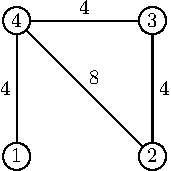
\includegraphics[scale=1.2]{img/graph1.pdf}}
\ \ \ \ \ \ \ \ \ \ \
L = \left(\begin{array}{rrrr}
     1  &   0  &   0  &  -1\\
     0  &   3  &  -1  &  -2\\
     0  &  -1  &   2  &  -1\\
    -1  &  -2  &  -1  &   4
\end{array}\right) 
$$
and the added redundant constraint $x_2x_3 + x_3x_4 + x_4x_2 \geq -1,$
 represents the triangle inequality for the triangle $(2,3,4)$ contained in the graph.


\subsection{SOCP relaxations}



Let $$\lambda_1\leq \cdots \leq \lambda_l \leq  0 < \lambda_{l+1} \leq \cdots \geq \lambda_n, $$
be the eigenvalues of matrix $L$ and let $q_1,\dots , q_n$ be the corresponding unit eigenvectors. Denote $L^- = -\sum_{j = 1}^{l}\lambda_j q_jq_j^T\succeq 0$.


Using the framework by Kim and Kojima [\ref{KimKojimaSOCPofNoncvxQOP}] which we have described in the Section \ref{SubsectionSOCPrelaxInOriginalVariable} we obtain following SOCP relaxation of max-cut
\begin{equation}
\begin{array}{ll}
\label{MaxCutSOCPRelax1}
\mbox{maximize} & t, \\
\mbox{subject to} & \frac{1}{4}x^TL^-x + \sum_{j=l+1}^n\lambda_jz_j + t \leq 0 , \\
&	x^Tq_jq_j^Tx - z_j \leq 0, \ (j = l+1,\dots ,n), \\
&  	x^Te_je_j^Tx \leq 1, \ (j = 1,\dots ,n), \\
& z_j \leq \sqrt{n}, \ (j = l+1,\dots ,n).
\end{array}
\end{equation}
Here, the bound for $z_j = q^T_jXq_j$ comes from the fact that $X_{ij}$ is either $+1$ or $-1,$ and $\Vert q \Vert_2 = 1.$

In fact, if graph $G$ has no loops, i.e. $w_{ii} = 0$ $\forall i\in V$ and all weights are nonnegative, then $L$ is diagonally dominant, since
$$L_{ii} = \sum_{j\in V} w_{ij} = \sum_{i\neq j} \vert L_{ij} \vert. $$
Hence, $L$ is positive semidefinite and $L^-=0.$ Therefore the quadratic term in the first constraint vanishes.



\subsubsection{An improvement for max-cut}
Authors Muramatsu and Suzuki [\ref{MuramatsuSuzukiANewSOCPrelaxForMaxCut}]
propose an improvement of this relaxation (especially for the max-cut) based on the problem structure. Their approach considers different choice of the matrices $C$ in the relaxation of semidefinite constraint $C\bullet X - x^TCx \geq 0$.

Denote 
\begin{eqnarray*}
u_{ij} &=& e_i + e_j, \\
v_{ij} &=& e_i - e_j.
\end{eqnarray*}
Their choice of matrices $C$ consist of the following 
\begin{eqnarray*}
e_ie_i^T, &\ & i = 1,\dots,n, \\
u_{ij}u_{ij}^T, &\ & [i,j]\in \mathcal{E}, \\
v_{ij}v_{ij}^T, &\ & [i,j]\in \mathcal{E},
\end{eqnarray*}
where $\mathcal{E}$ denotes the set of edges, in terms of entries of matrix $L$ the set $\mathcal{E} = \{[i,j] \ \vert \ i,j\in V,\ i\neq j, \ L_{ij}\neq 0\}$.
The corresponding quadratic constraints are 
\begin{eqnarray}
\label{muramatsuConstraint1}
x^Te_ie_i^Tx - e_ie_i^T\bullet X &\leq & 0, \ i = 1,\dots,n,\\ 
\label{muramatsuConstraint2}
x^Tu_{ij}e_{ij}^Tx - u_{ij}u_{ij}^T\bullet X &\leq & 0, \ [i,j]\in \mathcal{E},\\ 
\label{muramatsuConstraint3}
x^Tv_{ij}e_{ij}^Tx - u_{ij}v_{ij}^T\bullet X &\leq & 0, \ [i,j]\in \mathcal{E}. 
\end{eqnarray}
As Kim and Kojima in [\ref{KimKojimaSOCPofNoncvxQOP}], they also reduce the number of variables. In fact, since $X_{ii} = 1$ , the constraint (\ref{muramatsuConstraint1}) reduces to $x_i^2 \leq 1$.
By introducing the new variables 
\begin{eqnarray*}
s_{ij} &:= & u_{ij}^TXu_{ij},\ [i,j]\in \mathcal{E}, \\ 
z_{ij} &:= & v_{ij}^TXv_{ij},\ [i,j]\in \mathcal{E}, 
\end{eqnarray*}
they obtain a quadratic inequalities from (\ref{muramatsuConstraint2}) and (\ref{muramatsuConstraint3})
\begin{eqnarray*}
(x_i + x_j)^2 \leq s_{ij}, \ [i,j]\in \mathcal{E}, \\
(x_i - x_j)^2 \leq z_{ij}, \ [i,j]\in \mathcal{E}. 
\end{eqnarray*}
For those variables they have following bound
\begin{equation*}
s_{ij} + z_{ij} = X\bullet(u_{ij}u_{ij}^T - v_{ij}v_{ij}^T) = 2(X_{ii} + X_{jj}) = 4.
\end{equation*}

Furthermore, they prove following proposition
\prop \begin{equation}
\label{muramatsuPropositionL}
L = - \sum_{[i,j]\in \mathcal{E}} L_{ij}v_{ij}v_{ij}^T.
\end{equation}
\rm
\begin{proof}
 Let $$\delta_{ij} = e_i^Te_j = \left\lbrace \begin{array}{l}
1, \ \mbox{ if } i = j, \\
0, \ \mbox{ otherwise}.
\end{array}\right.$$
The $(k,l)$ th componen of the right-hand side of (\ref{muramatsuPropositionL}) is 
\begin{eqnarray*}
e_k^T\left(- \sum_{[i,j]\in \mathcal{E}} L_{ij}v_{ij}v_{ij}^T \right) e_l &=& - \sum_{[i,j]\in \mathcal{E}} L_{ij}e_k^T(e_i-e_j)(e_i-e_j)^Te_l \\
&=& - \sum_{[i,j]\in \mathcal{E}} L_{ij}(\delta_{ki}\delta_{il} + \delta_{kj}\delta_{jl} -  \delta_{ki}\delta_{jl} - \delta_{kj}\delta_{il}) \\
&=& \left\lbrace \begin{array}{ll}
- \sum_{[k,j]\in \mathcal{E}}L_{kj} & \mbox{ if } k = l ,\\
L_{kl} & \mbox{ if } [k,l]\in\mathcal{E}, \\
0 & \mbox{ otherwise.}
\end{array}\right. \\
&=& L_{kl}
\end{eqnarray*}
\end{proof}

Using the proposition the objective is rewritten as 
\begin{equation*}
\frac{1}{4}L\bullet X = -\frac{1}{4}\sum_{[i,j]\in \mathcal{E}} L_{ij}v_{ij}v_{ij}^T\bullet X = -\frac{1}{4} \sum_{[i,j]\in \mathcal{E}} L_{ij}v_{ij}^TXv_{ij} = - \sum_{[i,j]\in \mathcal{E}} L_{ij}z_{ij}.
\end{equation*}

Now with $X$ removed they obtain the following relaxation 
\begin{equation}
\begin{array}{ll}
\label{MaxCutSOCPRelax2}
\mbox{maximize} & - \frac{1}{4}\sum_{[i,j]\in \mathcal{E}} L_{ij}z_{ij}, \\
\mbox{subject to} & x_i^2\leq 1 , \ (i = 1,\dots ,n),\\
&	(x_i + x_j)^2 \leq s_{ij}, \ [i,j]\in \mathcal{E}, \\
& 	(x_i - x_j)^2 \leq y_{ij}, \ [i,j]\in \mathcal{E}, \\
& s_{ij} + z_{ij} = 4, \ [i,j]\in \mathcal{E}.
\end{array}
\end{equation}

They also propose adding a certain form of triangle inequalities into the relaxation (\ref{MaxCutSOCPRelax2}). 

\prop \label{MuramatsuTriangleIneq}
If $[i,j],\ [j,k],\ [k,l]\in\mathcal{E}$, then following inequalities are valid \rm
\begin{eqnarray*}
z_{ij} + z_{jk} + z_{ki} &\leq & 8, \\
z_{ij} + s_{jk} + s_{ki} &\leq & 8, \\
s_{ij} + s_{jk} + z_{ki} &\leq & 8, \\
s_{ij} + z_{jk} + s_{ki} &\leq & 8.
\end{eqnarray*}

\begin{proof}
Since $X_{ii} = 1 $, we have 
\begin{eqnarray*}
z_{ij} + z_{jk} + z_{ki} &=& v_{ij}^TXv_{ij} + v_{jk}^TXv_{jk} + v_{ki}^TXv_{ki} \\
 & = & 2(X_{ii} + X_{jj} + X_{kk}) - 2(X_{ij} + X_{jk} + X_{ki}) \\
 & = & 6 - 2(X_{ij} + X_{jk} + X_{ki}).
\end{eqnarray*}
From triangle inequality $X_{ij} + X_{jk} + X_{ki}\geq -1$ it follows that $z_{ij} + z_{jk} + z_{ki} \leq 8.$ The other three inequalities can be proved similarly.
\end{proof}

Putting all together (triangle inequalities and (\ref{MaxCutSOCPRelax2}) we have one more SOCP relaxation for max-cut
\begin{equation}
\begin{array}{ll}
\label{MaxCutSOCPRelax2+TriangleIneq}
\mbox{maximize} & - \frac{1}{4}\sum_{[i,j]\in \mathcal{E}} L_{ij}z_{ij}, \\
\mbox{subject to} & \ x_i^2\leq 1 , \ (i = 1,\dots ,n),\\
&  \left.\begin{array}{lcl}
	(x_i + x_j)^2 \leq s_{ij},  \\
 	(x_i - x_j)^2 \leq y_{ij},  \\
 	s_{ij} + z_{ij} = 4,  
 \end{array}\right\rbrace [i,j] \in\mathcal{E},\\
& \left.\begin{array}{lcl}
	z_{ij} + z_{jk} + z_{ki} &\leq & 8, \\
	z_{ij} + s_{jk} + s_{ki} &\leq & 8, \\
	s_{ij} + s_{jk} + z_{ki} &\leq & 8, \\
	s_{ij} + z_{jk} + s_{ki} &\leq & 8.
\end{array}\right\rbrace [i,j],\ [j,k],\ [k,l]\in\mathcal{E}.
\end{array}
\end{equation}


As the number of the variables in these relaxations (\ref{MaxCutSOCPRelax2}), (\ref{MaxCutSOCPRelax2+TriangleIneq}) depend highly on the number of edges in $\mathcal{E}$, it is expected that these relaxations will do better on the sparse graphs. Authors of [\ref{MuramatsuSuzukiANewSOCPrelaxForMaxCut}] also propose fixing the nodes with high degree first as a heuristic for branching in the branch and bound procedure in order to obtain a speed up by decreasing the number of variables.

\subsection{Mixed SOCP-SDP relaxation}

We will form a relaxation based on the approach by Burer, Kim and Kojima  [\ref{BurerKimKojimaFasterWeakerRelax}], which we have described in section \ref{SectionMixedSocpSDP}.

In this problem we are maximizing, therefore instead of looking for the smallest eigenvalue of we will need the largest one. Let  $\lambda_{0}$ be the largest eigenvalue of $L$.

%\rem Since for a graph without loops $L$ is positive semidefinite, $\lambda_{0}$ is also the eigenvalue with largest magnitude, this will allow us to find it faster.

By splitting the matrix $L$ we will rewrite the max-cut as follows
\begin{equation*}
\begin{array}{ll}
\mbox{maximize} & \frac{1}{4}\left[ \ x^T(L- \lambda_{0} I_n)x + \lambda_0x^TI_nx \ \right], \\
\mbox{subject to} & diag(X) = e .
\end{array}
\end{equation*}
And using the procedure from Section \ref{SectionMixedSocpSDP} we obtain a following relaxation 
%
%Now introducing the variable $X=xx^T$ and rewriting the convex term $$\lambda_0x^TI_nx = \lambda_0I_n\bullet X = \lambda_0tr(X)$$
%we have equivalent formulation
%\begin{equation}
%\begin{array}{ll}
%\mbox{maximize} & \frac{1}{4}\left[ \ x^T(L- \lambda_{0} I_n)x + \lambda_0Tr(X)\ \right], \\
%\mbox{subject to} & diag(X) = e ,\\
%& X = xx^T,
%\end{array}
%\end{equation}
%and relaxing the nonconvex constraint $X=xx^T$ as $X\succeq xx^T$ we obtain 
%\begin{equation}
%\begin{array}{ll}
%\mbox{maximize} & \frac{1}{4}\left[ \ x^T(L- \lambda_{0} I_n)x + \lambda_0Tr(X) \ \right], \\
%\mbox{subject to} & diag(X) = e ,\\
%&	X \succeq xx^T.
%\end{array}
%\end{equation*}
%This is accoding to the Proposition \ref{PropGronePSDcompletion} equivalent to 
\begin{equation*}
\begin{array}{ll}
\mbox{maximize} & \frac{1}{4}\left[ \ x^T(L- \lambda_{0} I_n)x + \lambda_0Tr(X) \ \right], \\
\mbox{subject to} & diag(X) = e ,\\
&	x_i^2\leq X_{ii} \ (i=1,\dots ,n).
\end{array}
\end{equation*}
Notice, that using the constraint $diag(X) = e$ we know that $Tr(X) = n$ and $x_i^2\leq X_{ii}$ reduces to $x_i^2\leq 1$. Finally we are left with  
\begin{equation}
\label{MaxCutMixedSocpSdp1}
\begin{array}{ll}
\mbox{maximize} & \frac{1}{4}\left[ \ x^T(L- \lambda_{0} I_n)x + \lambda_0n \ \right], \\
\mbox{subject to} & diag(X) = e ,\\
&	x_i^2\leq 1 \ (i=1,\dots ,n).
\end{array}
\end{equation}

\subsubsection{Block diagonal splitting}

Using the more general $\mathcal{C}$-block diagonal splitting of matrix $L$ by [\ref{BurerKimKojimaFasterWeakerRelax}], we will obtain another relaxation which was described in Section $\ref{SectionMixedSocpSDP}$. Now we will apply this technique to the max-cut.

Let $\mathcal{C}=\{C_1,\dots ,C_r\}$ be a partition of the indices $\{1, \dots ,n\}$. Let $M$ be a $n\times n$ matrix. We will denote $M(\mathcal{C})$ a $n\times n$ matrix with entries 
\begin{equation*}
M(\mathcal{C})_{ij} = \left\lbrace \begin{array}{ll}
M_{ij}, & \mbox{ if } i,j \mbox{ are in the same partition of }\mathcal{C},\\
0, & \mbox{ otherwise.}
\end{array}\right.
\end{equation*} 
We denote $\bar{M}(\mathcal{C}) = M-M(\mathcal{C})$ the matrix with all the complementary entries of $M$.
And denote $\lambda_{max}(M)$  the largest eigenvalue of $M$.

Let 
$$ D = L(\mathcal{C}) + \lambda_{max}(\bar{L}(\mathcal{C}))I .$$
We will be splitting the matrix $L$ as  $L = (L - D) + D$, because we are maximizing, we need $(L-D)$ to be negative semidefinite, which it indeed is
$$(L - D)= \bar{L}(\mathcal{C}) - \lambda_{max}(\bar{L}(\mathcal{C}))I \preceq 0.$$
Hence, we have the following mixed SOCP-SDP relaxation 
\begin{equation}
\label{MaxCutMixedSocpSdpR}
\begin{array}{ll}
\mbox{maximize} & \frac{1}{4}\left[ \ x^T(L-D)x + \sum_{j=1}^r D_{C_jC_j}\bullet X_{C_jC_j} \ \right], \\
\mbox{subject to} & diag(X) = e ,\\
&	X_{C_jC_j}\succeq x_{C_j}x_{C_j}^T \ (j=1,\dots ,r).
\end{array}
\end{equation}

In the special case when $r = n$ we have splitting
$L = (\bar{D}_L - \lambda_{max}(\bar{D}_L)I) + (D_L + \lambda_{max}(\bar{D}_L)I),$
where $D_L$ denotes the diagonal matrix with diagonal entries of $L$
and $\bar{D}_L = L - D_L$ denotes its complement.
Using that $diag(X) = e$ the resulting relaxation for this splitting is
\begin{equation}
\label{MaxCutMixedSocpSdpN}
\begin{array}{ll}
\mbox{maximize} & \frac{1}{4}\left[ \ x^T(\bar{D}_L - \lambda_{max}(\bar{D}_L)I)x + (e^TD_L + \lambda_{max}(\bar{D}_L)n) \ \right], \\
\mbox{subject to} & x_i^2 \leq 1, \ (i=1,\dots ,n).
\end{array}
\end{equation}

%%%%%%%%%%
\subsection{LP relaxations}
Following the form introduced in the Section \ref{SectionLPRelaxationsOfQCQP} we will form linear programming relaxations for max-cut. These relaxations are expected to be fast and produce weak bounds.

\subsubsection{Standard LP relaxation}
The standard relaxation is easily obtained form the SDP relaxation (\ref{MaxCutSDPRelax}) omitting the semidefinite constraint
\begin{equation}
\label{MaxCutLPRelaxStandard}
\begin{array}{ll}
\mbox{maximize} & \frac{1}{4}L\bullet X, \\
\mbox{subject to} & diag(X) = e ,\\
&	X=X^T.
\end{array}
\end{equation} 
This relaxation can be strengthened by adding the triangle inequalities (\ref{MaxCutTriangleInequalities}) resulting in 

\begin{equation}
\label{MaxCutLPRelaxTriag}
\begin{array}{ll}
\mbox{maximize} & \  \ \ \ \frac{1}{4}L\bullet X, \\
\mbox{subject to} &\ \ \ \ diag(X) = e, \\
&\ \ \	\ X=X^T ,\\
& \left.\begin{array}{rcl}
X_{ij} + X_{jk} + X_{ik} &\geq & -1, \\
X_{ij} - X_{jk} - X_{ik} &\geq & -1, \\
- X_{ij} - X_{jk} - X_{ik} &\geq & -1, \\
- X_{ij} + X_{jk} - X_{ik} &\geq & -1.
\end{array}\right\rbrace \ i,j,k \in V \\
\end{array}
\end{equation} 

\subsubsection{LP with RLT relaxation} 
As we have mentioned earlier in the Section \ref{SectionRLTinLP} a reformulation linearization techinque provides means to strengthen the relaxations. 

Since max-cut is symmetric in a sense that objective value for $x$ and $-x$ are equal, there is no loss of generality if we fix $x_1 = 1$, i.e. first vertex will belong to $S$. 

Let $X_1$ denote the first column of $X$. Putting $x_1 = 1$ into the original constraint $X = xx^T$ yields $X_1 = x$.
Therefore, even if we do not use variable $x$ explicitly, we can still form RLT constraints building links between first column (or first row due to symmetry) and the rest of the matrix $X$.


Since $x\in \mathbb{R}^n$ represents original variable $x\in \{0,1\}^n$ we can use box constraints 
$-e \leq x \leq e$
and obtain following RLT constraints linking $X$ and $X_1$ variables, as in (\ref{RLTrelax1}).
The resulting relaxation is (the matrix inequalities are considered element-wise)


\begin{equation}
\label{MaxCutLPRelaxRLT}
\begin{array}{ll}
\mbox{maximize} & \ \ \frac{1}{4}L\bullet X, \\
\mbox{subject to} & \ \ diag(X) = e , \\
		& \begin{array}{lcl}
		 X + X_1e^T + eX_1^T & \geq & -ee^T, \\
		 X - X_1e^T - eX_1^T & \geq & -ee^T, \\
		 X - X_1e^T + eX_1^T & \geq & -ee^T,
	\end{array}\\
 		&\  X=X^T.
\end{array}
\end{equation} 

Furthermore, we can use both RLT constraints and triangle inequalities
\begin{equation}
\label{MaxCutLPRelaxRLT+triangle}
\begin{array}{ll}
\mbox{maximize} & \ \ \ \ \frac{1}{4}L\bullet X, \\
\mbox{subject to} & \ \ \ \ diag(X) = e ,\\
& \ \ \ \ l\leq x \leq u,\ X=X^T, \\
& \\
& \left.\begin{array}{rcl}
X_{ij} + X_{jk} + X_{ik} &\geq & -1, \\
X_{ij} - X_{jk} - X_{ik} &\geq & -1, \\
- X_{ij} - X_{jk} - X_{ik} &\geq & -1, \\
- X_{ij} + X_{jk} - X_{ik} &\geq & -1,
\end{array}\right\rbrace \ i,j,k \in V \\
& \\
		& \ \ \ \begin{array}{lcl}
		 X + X_1e^T + eX_1^T & \geq & -ee^T, \\
		 X - X_1e^T - eX_1^T & \geq & -ee^T, \\
		 X - X_1e^T + eX_1^T & \geq & -ee^T.
	\end{array}
\end{array}
\end{equation} 






%%%%%%%%%%

\subsection{Doubly nonnegative relaxations}
For these relaxations we will need to reformulate max-cut as a problem with binary 0-1 variables. The max-cut problem 
(\ref{maxcut3}) is 
\begin{equation*}
\begin{array}{ll}
\mbox{maximize} & \frac{1}{4}x^TLx, \\
\mbox{subject to} & x\in\{-1,1\}^n .
\end{array}	
\end{equation*}
Using the linear transformation $x = 2y - e$ we obtain a problem with a 	
variable $y\in \{0,1\}^n.$ And the objective reduces to 
$$\frac{1}{4}x^TLx = \frac{1}{4}(2y-e)^TL(2y-e) = y^TLy - y^TLe + \frac{1}{4}e^TLe = y^TLy,$$
because $Le = 0$ from the definition of $L$ 
$$Le = diag(We)e - We = We - We = 0.$$
Hence the binary 0-1 formulation of max-cut is 
\begin{equation}
\label{MaxCut0-1}
\begin{array}{ll}
\mbox{maximize} & y^TLy, \\
\mbox{subject to} & y\in\{0,1\}^n .
\end{array}	
\end{equation}



\subsubsection{DNN relaxation}

A first DNN relaxation we will obtain from SDP by adding the nonnegative cone constraint, since $y\in\{0,1\}^n$, it holds that $y\geq 0$ and that $Y = yy^T \in \mathbb{N}^n$. 
Therefore we can relax $Y = yy^T$ as $Y\succeq yy^T$ and $Y\in\mathbb{N}^n$.
We will also use the constraint on diagonal entries $Y_{ii} = y_i^2 = y_i$. Hence we get the following relaxation
\begin{equation*}
\begin{array}{ll}
\mbox{maximize} & L\bullet Y, \\
\mbox{subject to} & diag(Y) = y , \\
				& Y\succeq yy^T, \\
				& Y\in\mathbb{N}^n.
\end{array}	
\end{equation*}
Which can be easily rewritten, using the Schur complement lemma (see Theorem \ref{SchurCompl} in the Appendix) with the doubly nonnegative variable in $ \mathbb{S}^{n+1}_+ \cap \mathbb{N}^{n+1}$. 
%Denote 
%$$\bar{L} = \left(\begin{array}{ll} 0 & 0^T \\ 0 & L \end{array}\right), \ \ \ \mbox{ and } \ \ \ 
%Z = \left(\begin{array}{ll} 1 & y^T \\ y & Y \end{array}\right).$$
The resulting relaxation is 
\begin{equation}
\label{MaxCutDNNRelax1}
\begin{array}{ll}
\mbox{maximize} & \ L\bullet Y, \\
\mbox{subject to} & \ diag(Y) = y , \\
				& \left(\begin{array}{ll} 1 & y^T \\ y & Y \end{array}\right)\in\mathbb{S}^{n+1}_+ \cap \mathbb{N}^{n+1}.
\end{array}	
\end{equation}


\subsubsection{Stronger DNN relaxation}
Following the procedure by Kim and Kojima [\ref{KimKojimaLagrangianDNNRelaxation1}], which we have described in the Section \ref{SectionLagrangianDNNrelax}, we fist add the slack variables $u\in\{0,1\}^n$ as a complementary 0-1 variables to $y$
\begin{equation}
\label{MaxCut complementarity formulation}
\begin{array}{ll}
\mbox{maximize} &  L\bullet yy^T, \\
\mbox{subject to} & y_iu_i = 0, \ (i = 1,\dots ,n), \\
				& y + u = e, \\
				& y\geq 0, \ \ u\geq 0.
\end{array}	
\end{equation}
Then introducing the matrix variables $Y = yy^T$,  $U = uu^T$ and $W = uy^T$  and relaxaing them we receive the following relaxation
\begin{equation}
\label{MaxCutDNNRelax2}
\begin{array}{ll}
\mbox{maximize} &  L\bullet Y, \\
\mbox{subject to} & y + u = e, \\
				& diag(Y) = y, \ \ \ diag(U) = u, \ \ \ diag(W) = 0, \\
				& \left(\begin{array}{lll}
				1 & y^T & u^T \\ 
				y & Y 	& W^T \\
				u & W 	& U
				\end{array}\right) \in\mathbb{S}^{2n+1}_+ \cap \mathbb{N}^{2n+1}.
\end{array}	
\end{equation}
This formulation has more variables than (\ref{MaxCutDNNRelax1}), but is stronger, at least because the variables $y$ are not only nonnegative, but also from nonneqativity of $u$ we have that $y\leq 1$. Furthermore, the semidefinite constraint also provides better links between these variables. In fact, if doubly nonnegative constraint in (\ref{MaxCutDNNRelax2}) would be replaced by the completely positive constraint, it would be an equivalent formulation of the original problem (\ref{MaxCut0-1}). This is due to results by Arima, Kim and Kojima [\ref{ArimaKimKojimaQCQPforCPP}].

\subsubsection{Lagrangian DNN relaxation}
We will derive Lagrangian DNN relaxation for (\ref{MaxCut complementarity formulation}), using the procedure form Section \ref{SectionLagrangianDNNrelax}.  
Let $A = (-e \ I_n \ I_n),$ \ $Q_1 = A^TA,$ 
$$ 
H_0 = \left(\begin{array}{lll}
1 & 0^T & 0^T \\
0 & 0	& 0 \\
0 & 0	& 0
\end{array}\right), \ \ \
Q_2 = \left(\begin{array}{lll}
0 & 0^T & 0^T \\
0 & 0	& I_n \\
0 & I_n	& 0
\end{array}\right), 
$$ 
$$
Q_0 = \left(\begin{array}{lll}
0 & 0^T  & 0^T \\
0 & L & 0\\
0 & 0 & 0
\end{array}\right)
\ \ \mbox{and } \ \ \ Z = \left(\begin{array}{lll}
z_0 & y^T  & u^T \\
y & yy^T & yu^T \\
u & uy^T & uu^T
\end{array}\right). 
$$
We can enforce $z_0 = 1$ by $Z\bullet H_0 = 1$. Then for $y,u\in \mathbb{R}^n_+$ it holds that 
$y+u = e$ is equivalent to $Q_1\bullet Z = 0$ and 
the complementarity constraints $y_iu_i = 0$ for $i = 1,\dots ,n$ are equivalent to $Q_2\bullet Z = 0$. Since both matrices $Q_1,Q_2$ are nonnegative and so is $Z$, then $Q_1\bullet Z\geq 0$ and $Q_2\bullet Z\geq 0$. Therefore two constraints $Q_1\bullet Z=0$ and $Q_2\bullet Z=0$ can be rewritten as single constraint $H_1\bullet Z = 0$ for $H_1 = Q_1 + Q_2$. 

The structure of $Z$ is equivalent to $Z$ being positive rank 1 matrix
$$Z\in\Gamma^{2n+1} = \{ xx^T \ \vert \ x\in\mathbb{R}^{2n+1}_+\}. $$ 
Now we can rewrite the problem (\ref{MaxCut complementarity formulation}) in he new variable $Z$ as 	
\begin{equation*}
\begin{array}{ll}
\mbox{maximize} &  Q_0\bullet Z, \\
\mbox{subject to} & H_0 \bullet Z = 1, \ \ \ H_1\bullet Z = 0, \\
				& Z \in \Gamma^{2n+1}.
\end{array}	
\end{equation*}

Relaxing the cone $\Gamma^{2n+1}$ with nonnegative cone $\mathbb{S}^n_+ \cap \mathbb{N}^n$ we obtain a DNN relaxation (equivalent with (\ref{MaxCutDNNRelax2})). And for chosen $\lambda$ we obtain following Lagrangian relaxations
\begin{eqnarray}
\label{MaxCutDNN3p}
L^p(\lambda) &:=& \min \{ Q_0\bullet Z  - \lambda H_1\bullet Z\ \vert \ H_0\bullet Z = 1, \ Z\in \mathbb{S}^n_+ \cap \mathbb{N}^n \}, \\
\label{MaxCutDNN3d}
L^d(\lambda) &:=& \max \{ y_0\ \vert \  - Q_0 + \lambda H_1 + y_0H_0  \in \mathbb{S}^n_+ + \mathbb{N}^n \}.
\end{eqnarray}

\rem We have formed a primal dual pair according to (\ref{LagrangianDNNPrimalDualPair1})-(\ref{LagrangianDNNPrimalDualPair2}) with $\mathcal{K}= \mathbb{S}^n_+ \cap \mathbb{N}^n $ and $\mathcal{K}^*= \mathbb{S}^n_+ + \mathbb{N}^n $ (See Example \ref{ExDualCones} in the Appendix).
Since we are maximizing, the signs differ from (\ref{LagrangianDNNPrimalDualPair1})-(\ref{LagrangianDNNPrimalDualPair2}).
%%%%%%%%%












%TODO: other combinatorial problems i.e. QAP, stable set, knapsack, ...
%
%\section{QAP}
%
%\section{Stable set}
%
%\section{Knapsack}
%





\chapter{Computational comparison}

In this section we will try to compare all of the methods we have managed to formulate for max-cut in the Section \ref{SectionMaxCutRelaxation}.

All of the computations are done in the {\tt Matlab} environment using the {\tt cvx library} with an open source solver {\tt SeDuMi.} Used machine had an {Intel Core i7-4710HQ 2.50GHz CPU} and 16GB memory.
Our code is available on GitHub repository\footnote{{\tt https://github.com/matus-stehlik/conic\_relaxations}} together with this thesis.  

We will refer to used methods by following abbreviations.
\bigskip

\begin{tabular}{|c|c|c|c|c|c|c|c|}
\hline
sdp & 
sdp rlt &	
sdp tri &	
socp1 & 
socp2 &
socp3 &	
mix1 & 
mix2 
\\ \hline
(\ref{MaxCutSDPRelax}) & 
(\ref{MaxCutSDP+RLTRelax}) & 
(\ref{MaxCutSDPRelax}) + (\ref{MaxCutTriangleInequalities}) & (\ref{MaxCutSOCPRelax1}) & 
(\ref{MaxCutSOCPRelax2}) & 
(\ref{MaxCutSOCPRelax2+TriangleIneq}) &
(\ref{MaxCutMixedSocpSdp1}) &
(\ref{MaxCutMixedSocpSdpN}) \\
\hline
\end{tabular}

\begin{tabular}{|c|c|c|c|c|c|c|c|c|}
\hline
mixr $r$ &
lp1 &
lp2 &
lp3 &
lp4 &
dnn1 &
dnn2 &
dnn3p &
dnn3d 	
\\ \hline
(\ref{MaxCutMixedSocpSdpR}) given $r$ &
(\ref{MaxCutLPRelaxStandard}) &
(\ref{MaxCutLPRelaxTriag}) &
(\ref{MaxCutLPRelaxRLT}) &
(\ref{MaxCutLPRelaxRLT+triangle}) &
(\ref{MaxCutDNNRelax1}) &
(\ref{MaxCutDNNRelax2}) &
(\ref{MaxCutDNN3p}) &
(\ref{MaxCutDNN3d}) \\
\hline
\end{tabular}

\bigskip


Since we are going to compare a long list of methods, we did not manage to optimize each of their implementations, nor solving algorithms. While we are using the {\tt cvx library} with the {\tt SeDuMi} solver, the quality of bounds should not be affected by the flaws of our implementation up to the presented precision. However, the running times are largely affected, since, for each class of methods, we are not using the best-known state of the art algorithms, but only a universal solver, which is more suitable for some classes than for the others. Namely LP and SDP relaxations are expected to have good performance because they are widely used classes. On the other hand, SOCP and DNN relaxations will probably take more time to solve then they would need using a specialized algorithms and efficient implementations.

\rem We would like to emphasize especially that our poor time performance of the DNN3p-DNN3d pair compared to SDP is purely due to our implementation. Efficient algorithms for solving this pair of problems have recently been proposed by Arima, Kim, Kojima and Toh [\ref{KimKojimaLagrangianDNNRelaxation1}, \ref{ArimaKimKojimaRobustLagrangianDNN}]. Their reported performance seems to be superior to SDP both in time and quality of the bounds.

In the comparison, we will therefore focus firstly on the quality of the produced bounds and secondly on the running time.

In the first section, we will compare all the relaxation methods using the small ($n=20$) generated instances of max-cut. 

Next we will consider the medium sized max-cut instances ($n\in\{60, 80, 100\})$, for all the methods that we are able to solve in reasonable time  (in our implementation).

After this round we will choose only fast methods to compare using the large scale instances ($n\in\{100,200,\dots, 600\})$. 


Last but not least, we will introduce the branch and bound framework, which provides a way to solve (not only) combinatorial problems to optimality using bounds obtained by solving relaxed problems. Additionally we will try to compare the performance of chosen methods in this procedure for max-cut.




\begin{figure}
\centering
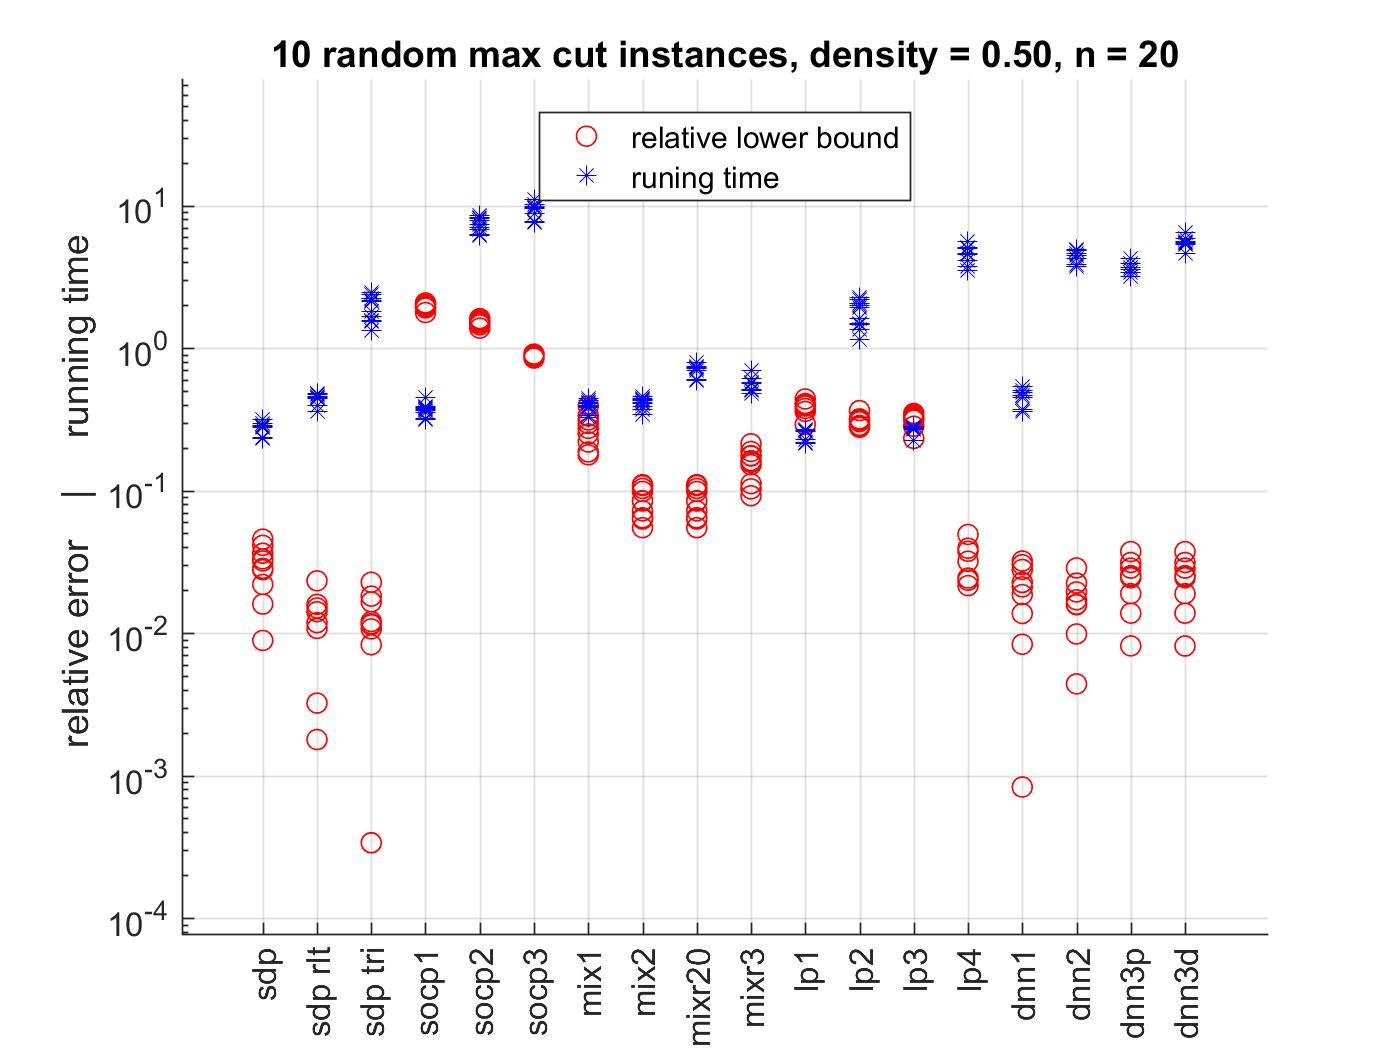
\includegraphics[scale=0.27]{img/comp0_d50_n20.jpg}
\caption[Comparison of relaxations - small, dense instances of max-cut 1]{Comparison of the relaxation methods for the small sized random generated instances max-cut with density $50\%$ and $n=20$.}
\label{comp0_d50_n20}

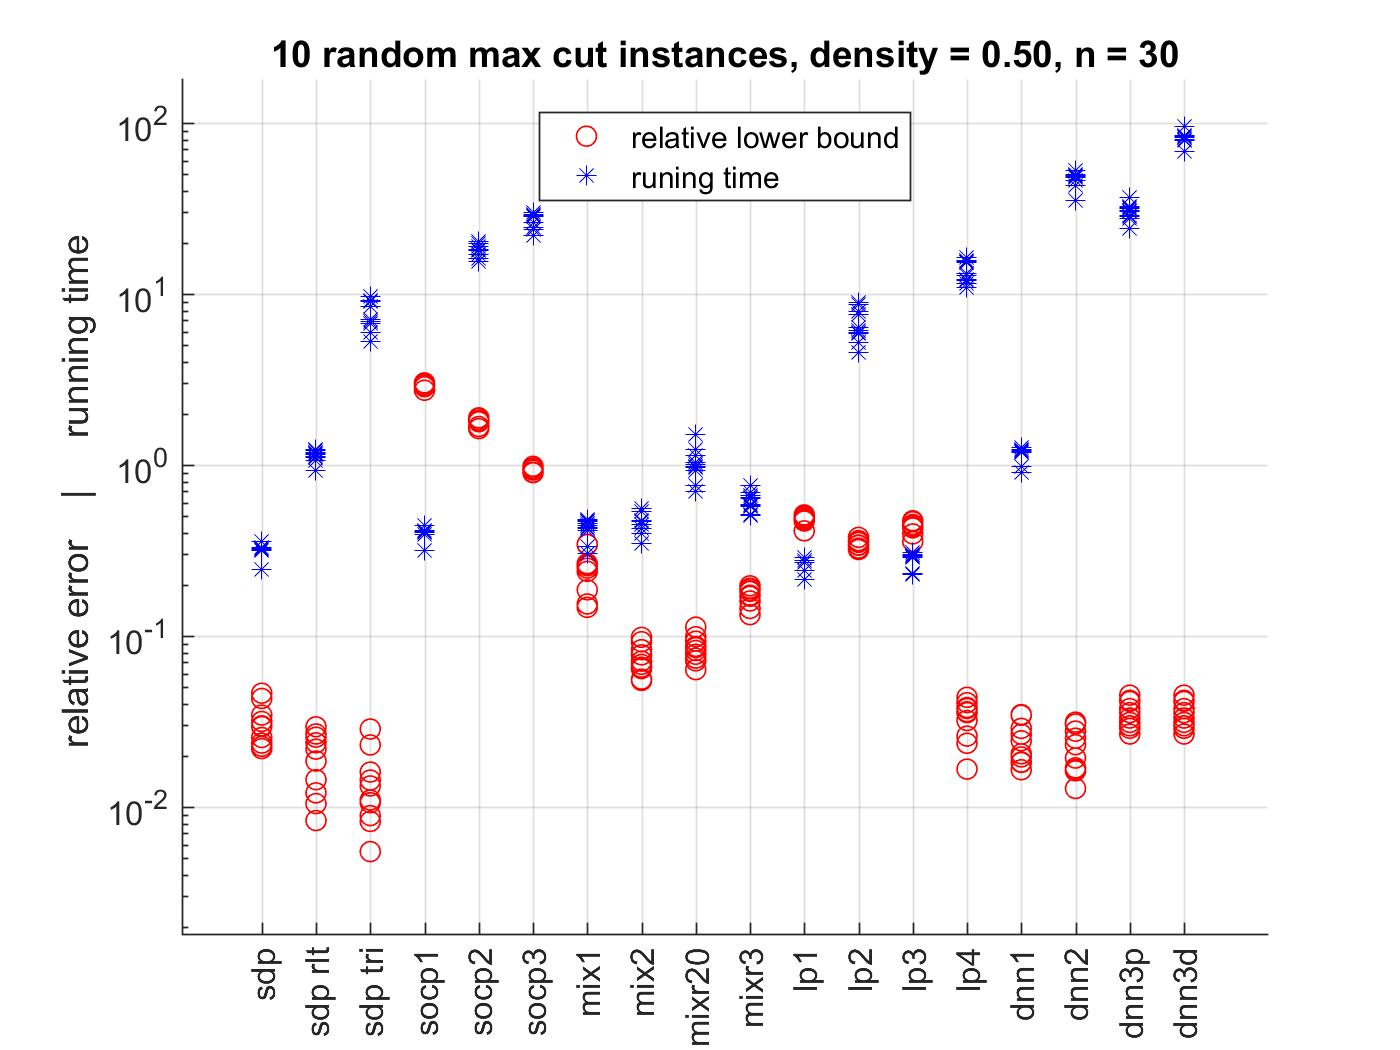
\includegraphics[scale = 0.27]{img/comp0_d50_n30.jpg}
\caption[Comparison of relaxations - small, dense instances of max-cut 2]{Comparison of the relaxation methods for the small sized random generated instances max-cut with density $50\%$ and $n=30$.}
\label{comp0_d50_n30}
\end{figure}
%\begin{figure}
%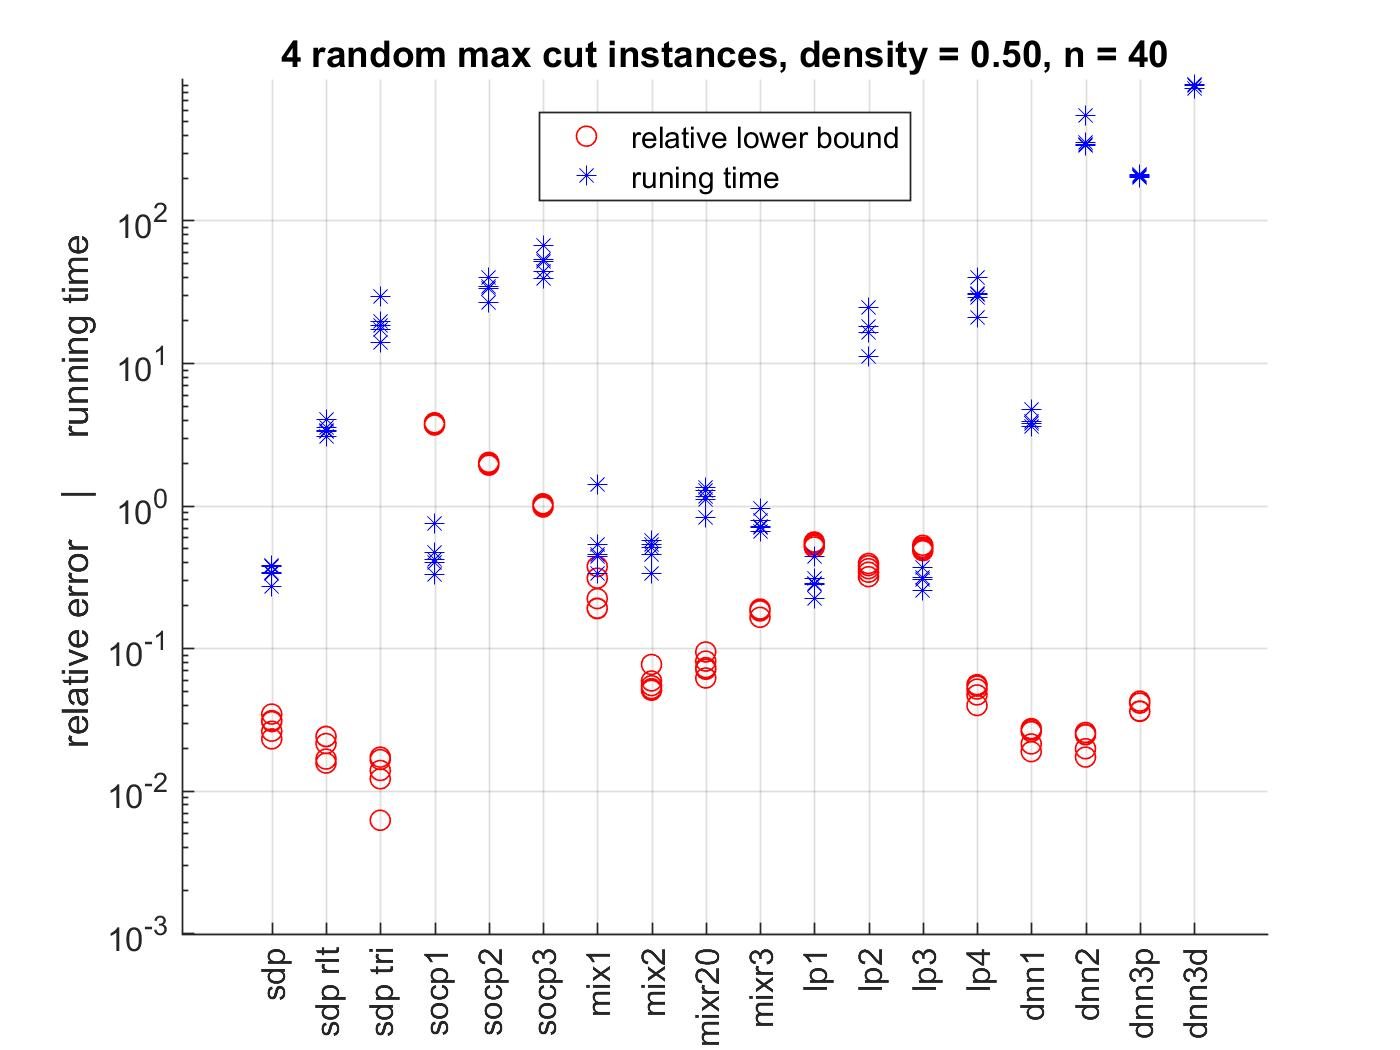
\includegraphics[scale=0.27]{img/comp0_d50_n40.jpg}
%\caption[Comparison of relaxations - small, dense instances of max-cut 3]{Comparison of the relaxation methods for the small sized random generated instances max-cut with density  $50\%$ and $n=40$.}
%\label{comp0_d50_n40}
%\end{figure}

\begin{figure}
\centering
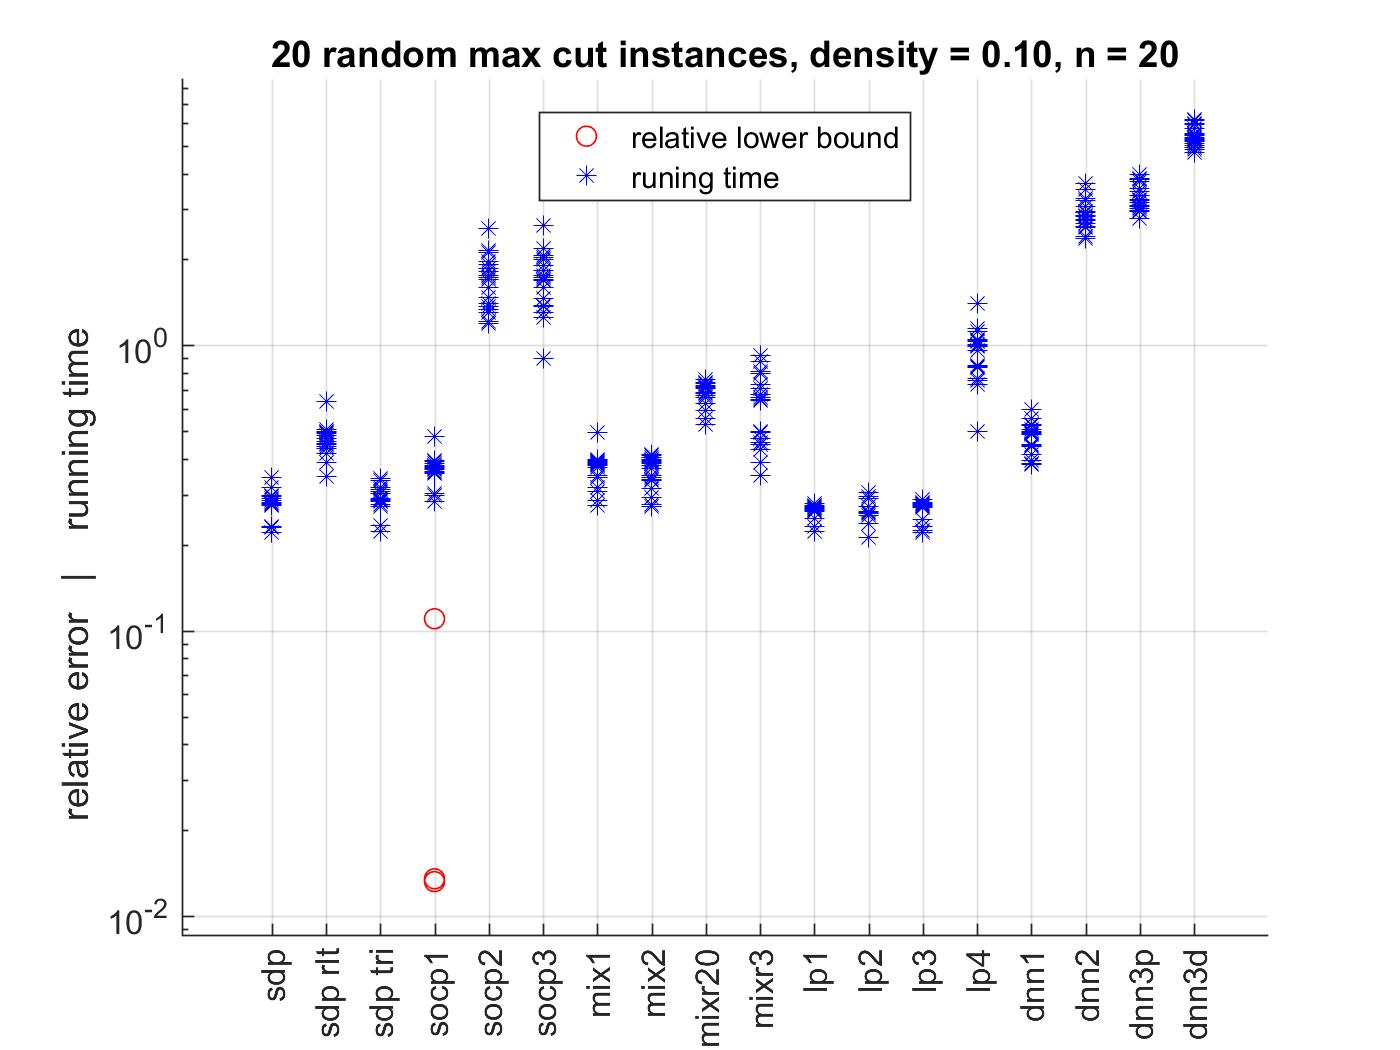
\includegraphics[scale = 0.27]{img/comp0_d10_n20.jpg}
\caption[Comparison of relaxations - small, sparse instances of max-cut]{Comparison of the relaxation methods for the small sized random generated instances max-cut with density $10\%$ and $n=20$. On the logarithmic scale we only see nonzero relative errors. All missing red circles represent the exact bounds.}
\label{comp0_d10_n20}
\end{figure}




\begin{figure}
\centering
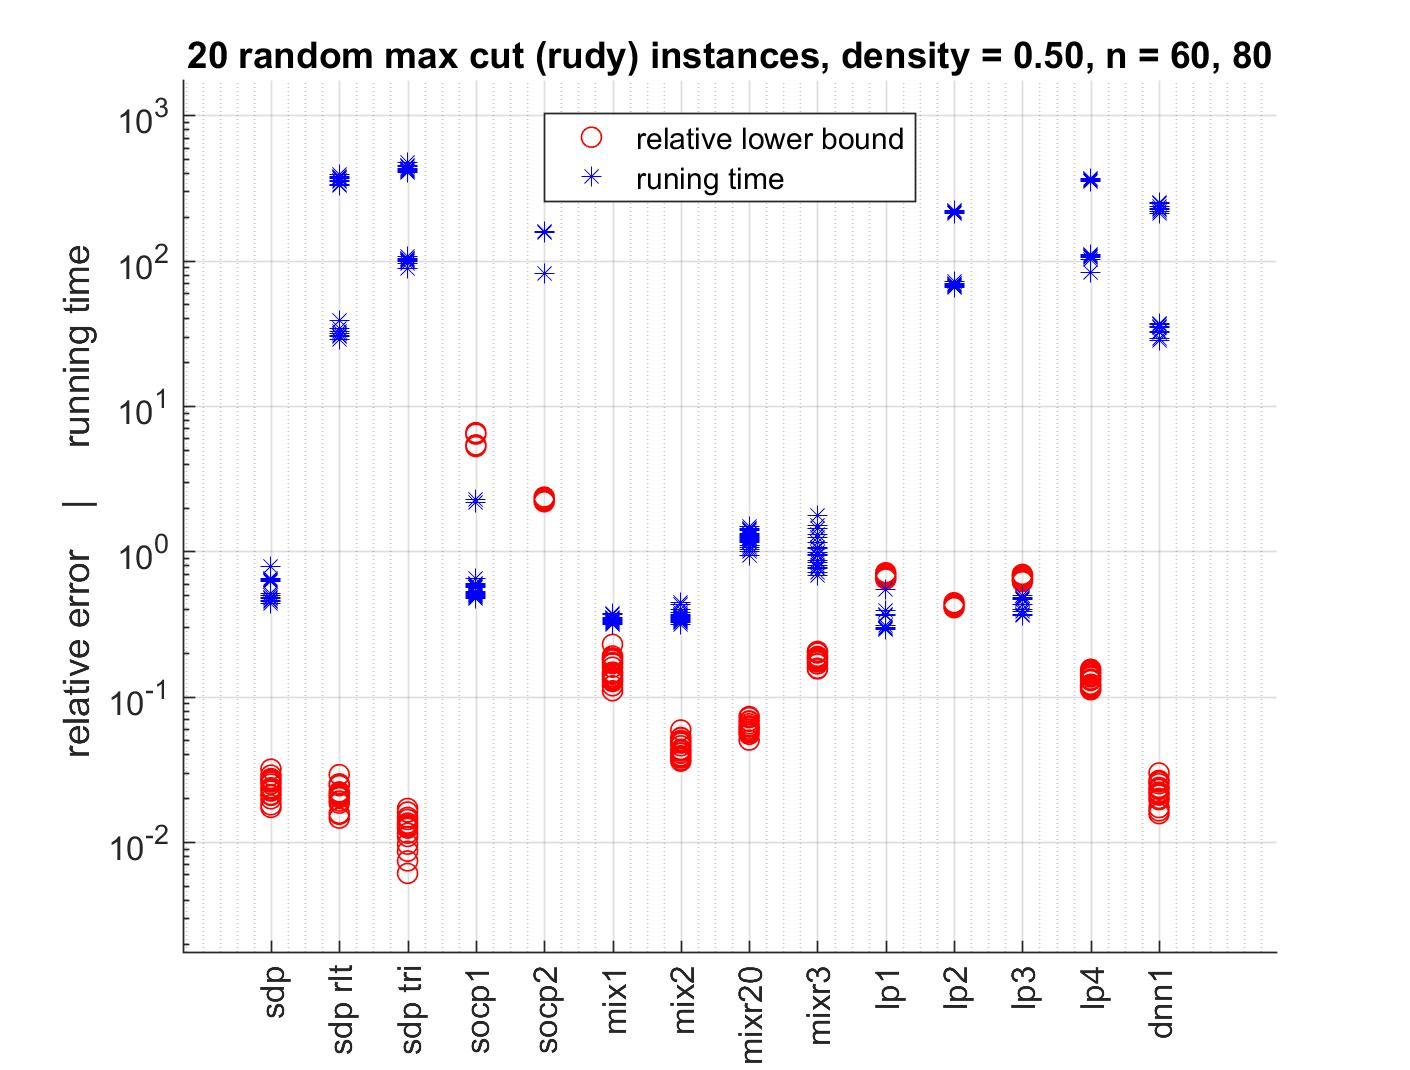
\includegraphics[scale=0.27]{img/comp1.jpg}
\caption[Comparison of relaxations - medium, dense instances of max-cut]{Comparison of the relaxation methods on the medium sized max-cut Rudy instances {\tt g\_05\_60, g\_05\_80,} from the Biq Mac library [\ref{BiqMacLib}], with density  $50\%$, unit edge weights and $n=60,\ 80$.} 
\label{comp1}
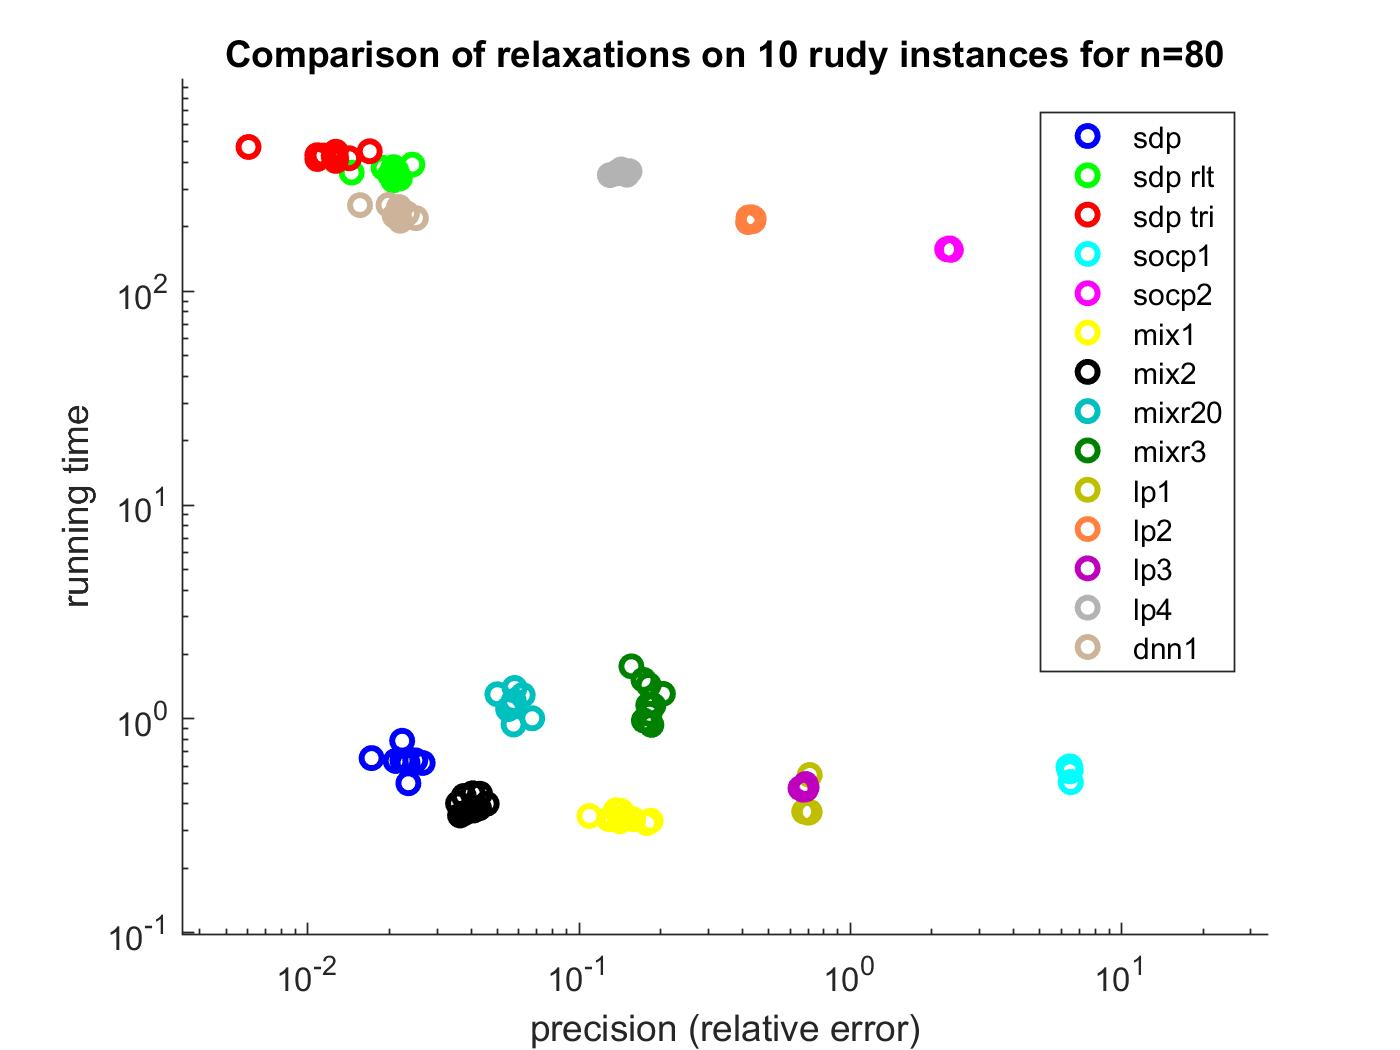
\includegraphics[scale=0.27]{img/comp1_segments.jpg}
\caption[Comparison of relaxations - a time-precision trade off]{A time-precision trade off on rudy instances for $n=80$.}
\label{comp1TradeOff}
\end{figure}



\section{Single bound comparison}

As noted above, in the comparison we will focus on the quality of the bounds (relative errors) and the speed (running time) of given methods.

The relative errors for the produced bounds are computed as 
\begin{equation}
\label{relative_error}
err = \frac{\theta_{relax} - \hat{\theta}}{\hat{\theta}},
\end{equation}
where $\hat{\theta}$ is the optimal value of the original problem and $\theta_{relax}$ is the computed upper bound (an optimal value of the relaxed problem). 

In order to capture both the large diversity of relaxation method classes and the small distinctions between methods of similar performance in a single graph, we are using a logarithmic scale for relative errors and running time. 



\subsection{Small sized instances}
All of the mentioned methods were compared using a small generated instnces of max-cut with integer edge weights $1\leq w_{ij}\leq 50$
and various densities. 

For each instance the optimal value was obtained by our branch and bound method. 

For a small density $10\%$ most of the produced bounds were exact (see Figure \ref{comp0_d10_n20}). 
As the density grows, the portion of exact bounds decreases. In the other graphs with density $50\%$ very few exact bounds were achieved.

In the figures \ref{comp0_d50_n20}, \ref{comp0_d50_n30}, we can see that adding the valid RLT inequalities (sdp rlt, lp3, lp4) or triangle inequalities (sdp tri, socp3, lp2, lp4), improves bounds but also increases the run time.

Suprisingly, SOCP relaxations (socp1, socp2, socp3) have very poor performance, at least in our implementation.


Now lets focus on the changes with the size of the problem. In the figures \ref{comp0_d50_n20}, \ref{comp0_d50_n30} one can see that while quality of the bounds stays about the same, the time complexity for some of the methods grows rapidly. Namely the SOCP relaxation with triangle inequalities (socp3) and DNN relaxations (dnn2, dnn3p, dnn3d). The former grows rapidly probably due to large number of triangle inequalities and the latter due to not using an efficient algorithm for DNN. From the practical reasons we are going to exclude these methods from further considerations on medium sized problems.





\subsection{Medium sized instances}

We have chosen all the methods with reasonable running time to compare on the $n=60$ and $n=80$ instances. See the Figure \ref{comp1}.

An interesting observation is that for some methods (sdp rlt, sdp tri, socp2, lp2, lp4, dnn1) the run times are well separated for $n=60$ and $n=80$ instances. On the other hand, the bounds seem to be stable.

Finally we can see in the Figure \ref{comp1} that mixed SOCP-SDP relaxations are getting slightly faster than SDP and that their bounds are quite good, especially mix2 seems to perform very well. 
Similar to the small instances, SOCP methods (socp1, socp2) do not produce reasonable bounds. 

An interesting comparison is captured in Figure \ref{comp1TradeOff}.
One can see the time-precision trade off for the methods close to axes. Also it is obvious that some methods are inferior in both time and precision to others.
The empty space for the high precision - medium speed methods can be filled either by including only a portion of the valid inequalities, or as we suggest later, by using the fast relaxation methods in the branch and bound framework.




\begin{center}
\begin{figure}
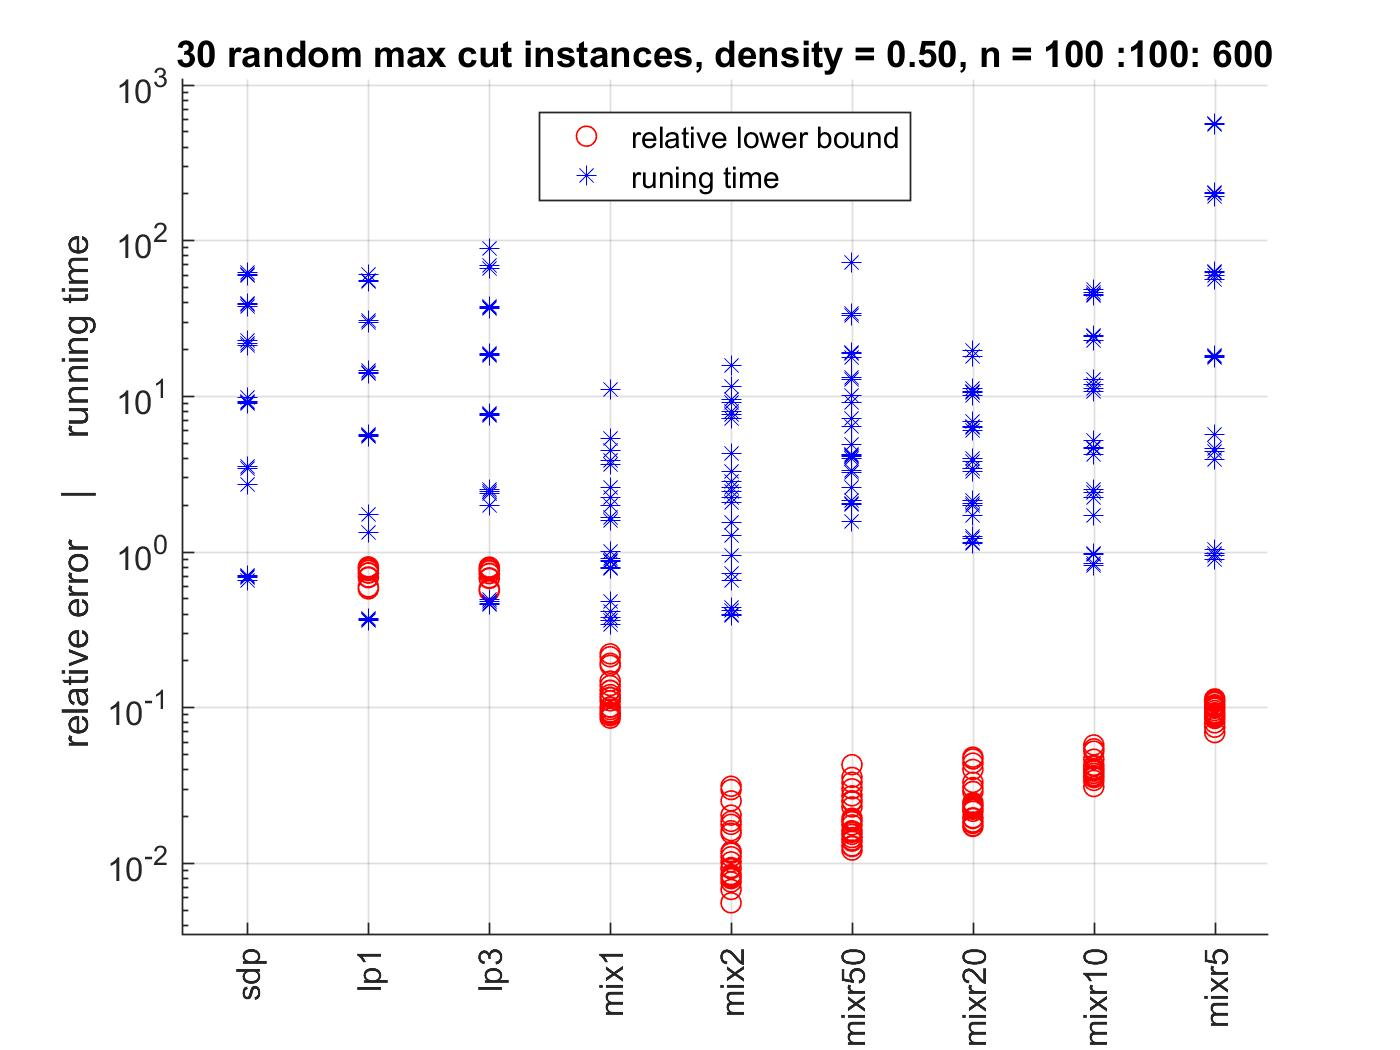
\includegraphics[scale=0.27]{img/comp3.jpg}
\caption[Comparison of relaxations - large, dense instances of max-cut 1]{Comparison of the relaxation methods on the large max-cut instances with density  $50\%$, integer edge weights between 1 and 50, $n=100,200\dots ,600$. The relative error is approximated using SDP relaxation as benchmark and computing errors relatively to the bounds produced by sdp.} 
\label{comp3}

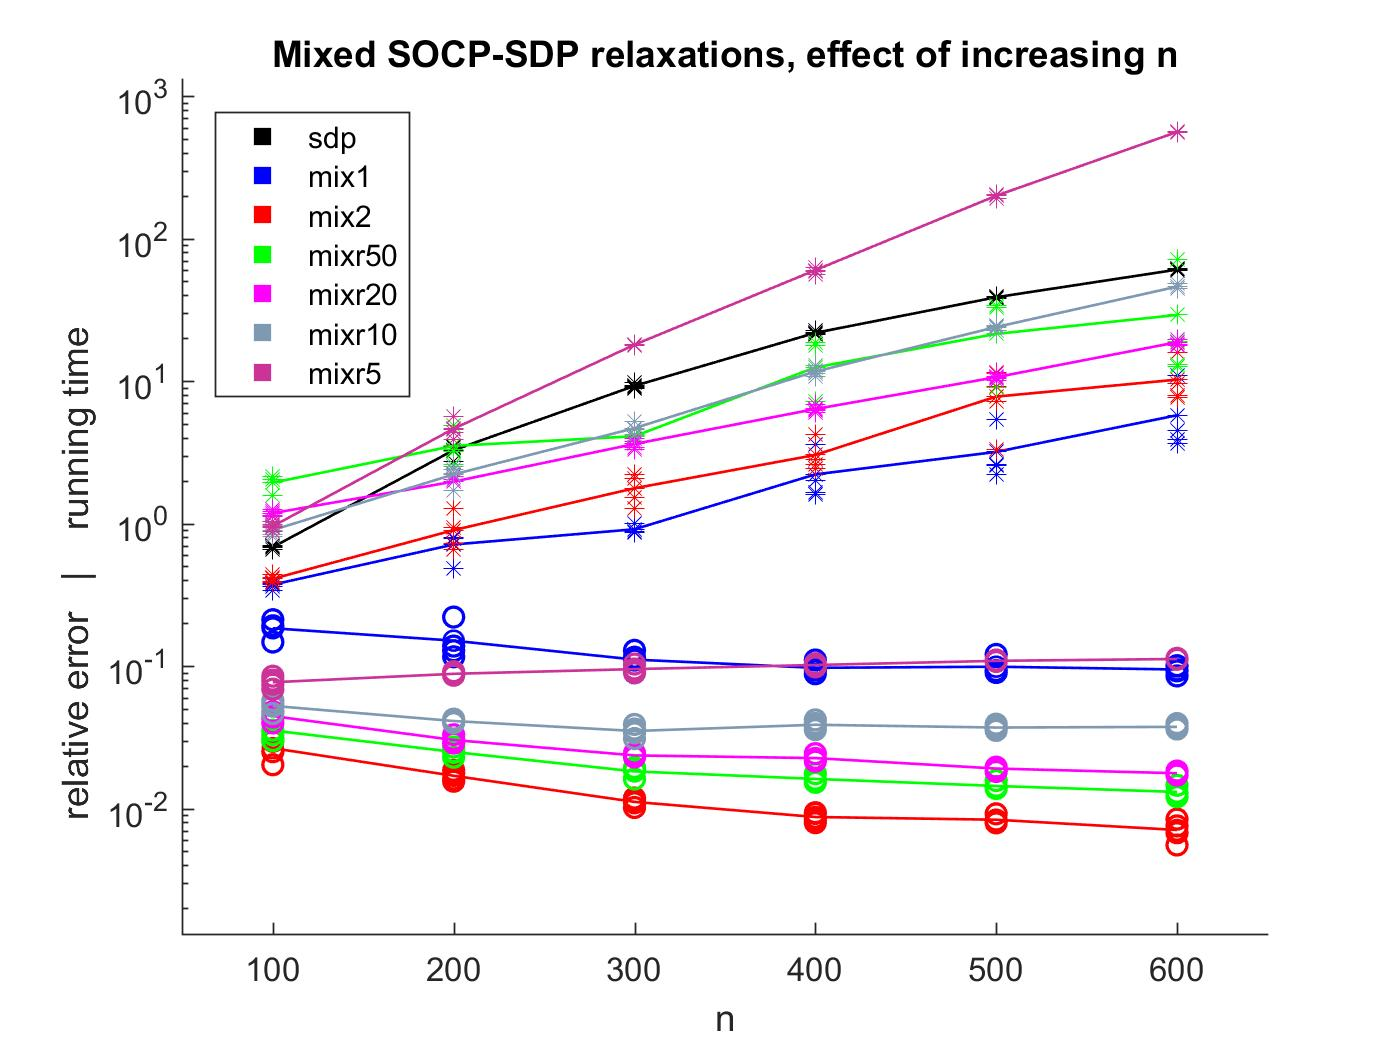
\includegraphics[scale=0.27]{img/comp_mix_n_100-600.jpg}
\caption[Comparison of relaxations - large, dense instances of max-cut 2]{Comparison of the mixed relaxation methods on the large max-cut instances with density  $50\%$, integer edge weights between 1 and 50, $n=100,200\dots ,600$. The relative error is approximated using SDP relaxation as benchmark and computing errors relatively to the bounds produced by sdp. Lines are connecting the mean values for each size and mothod.} 
\label{comp3size}
\end{figure}
\end{center}
%\begin{center}
%\begin{figure}
%\begin{minipage}{1\textwidth}
%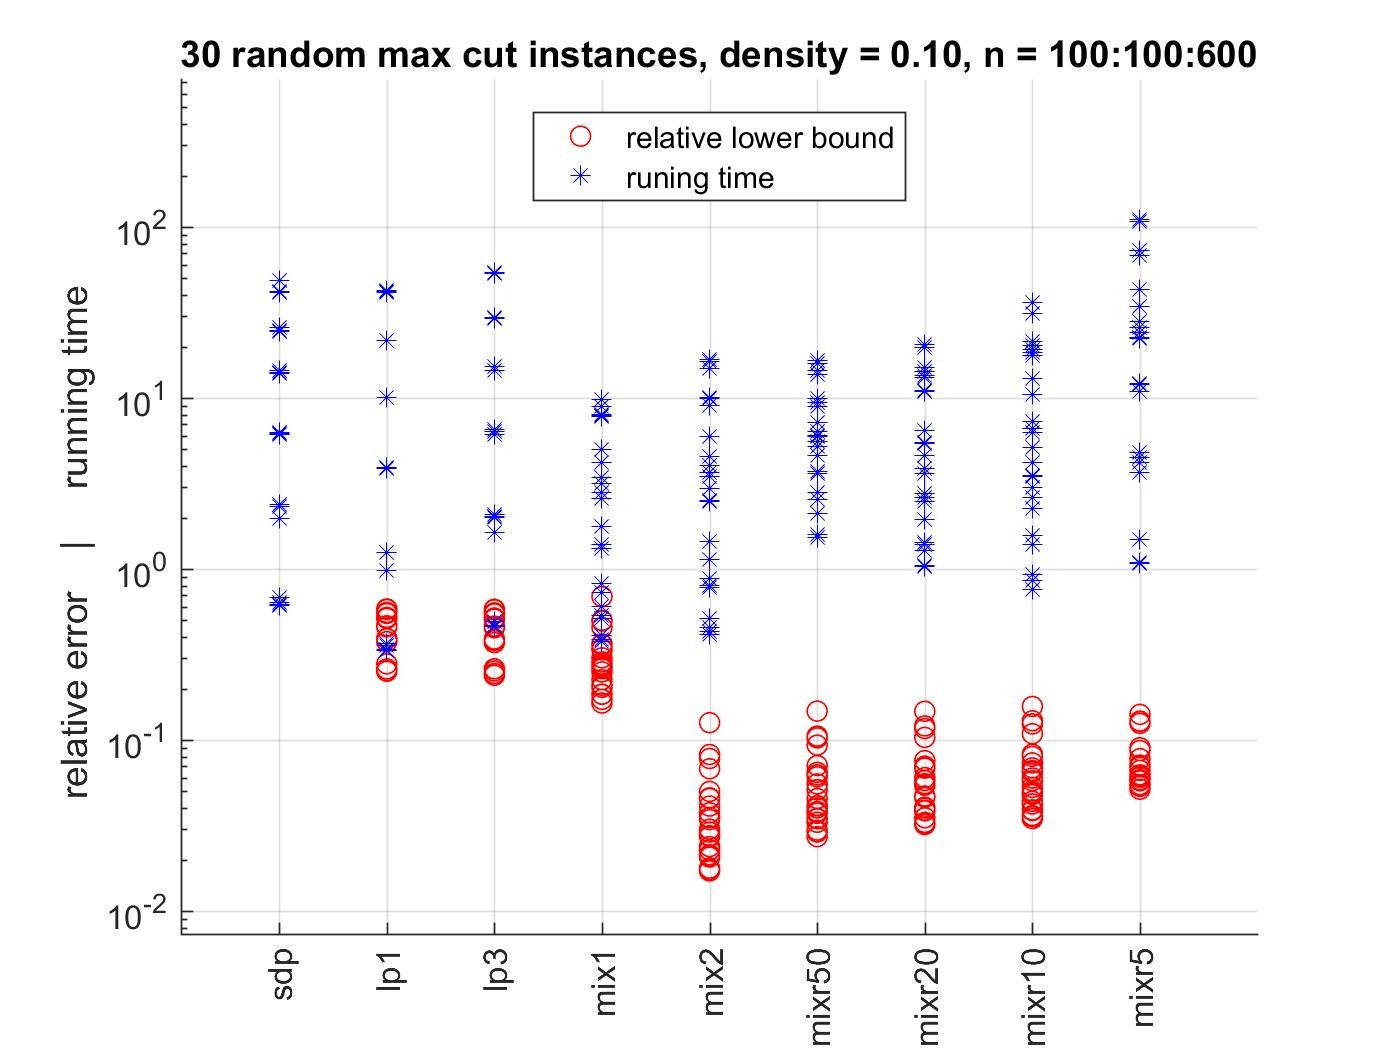
\includegraphics[scale=0.27]{img/comp3_sparse.jpg}
%\caption[Comparison of relaxations - large, sparse instances of max-cut 1]{Comparison of the relaxation methods on the large max-cut instances with density  $10\%$, integer edge weights between 1 and 50, $n=100,200\dots ,600$. The relative error is approximated using SDP relaxation as benchmark and computing errors relatively to the bounds produced by sdp.} 
%\label{comp3_sparse}
%\end{minipage}
%\end{figure}
%\end{center}

\begin{figure}
\centering
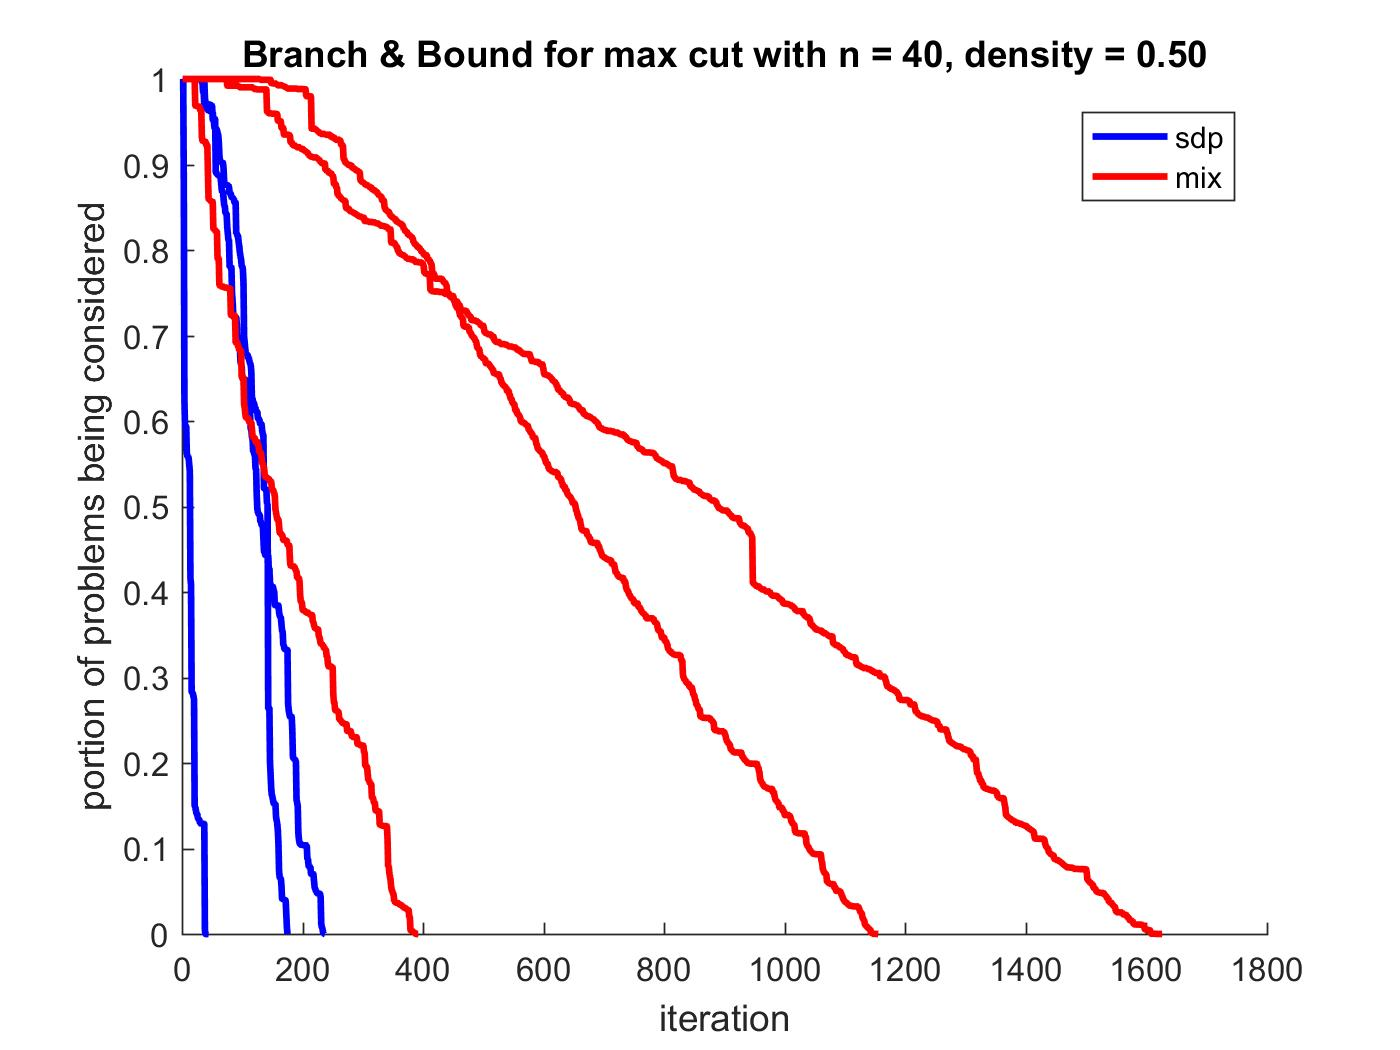
\includegraphics[scale=0.25]{img/compbnb_n40_d50_cons4.jpg}
\caption[Branch and bound comparison of the relaxation methods]{Branch and bound comparison of the relaxation methods SDP and mixed SOCP-SDP relaxation, on 3 random generated instances. }
\label{Figurebnb3}
\end{figure}



\begin{figure}
\centering 

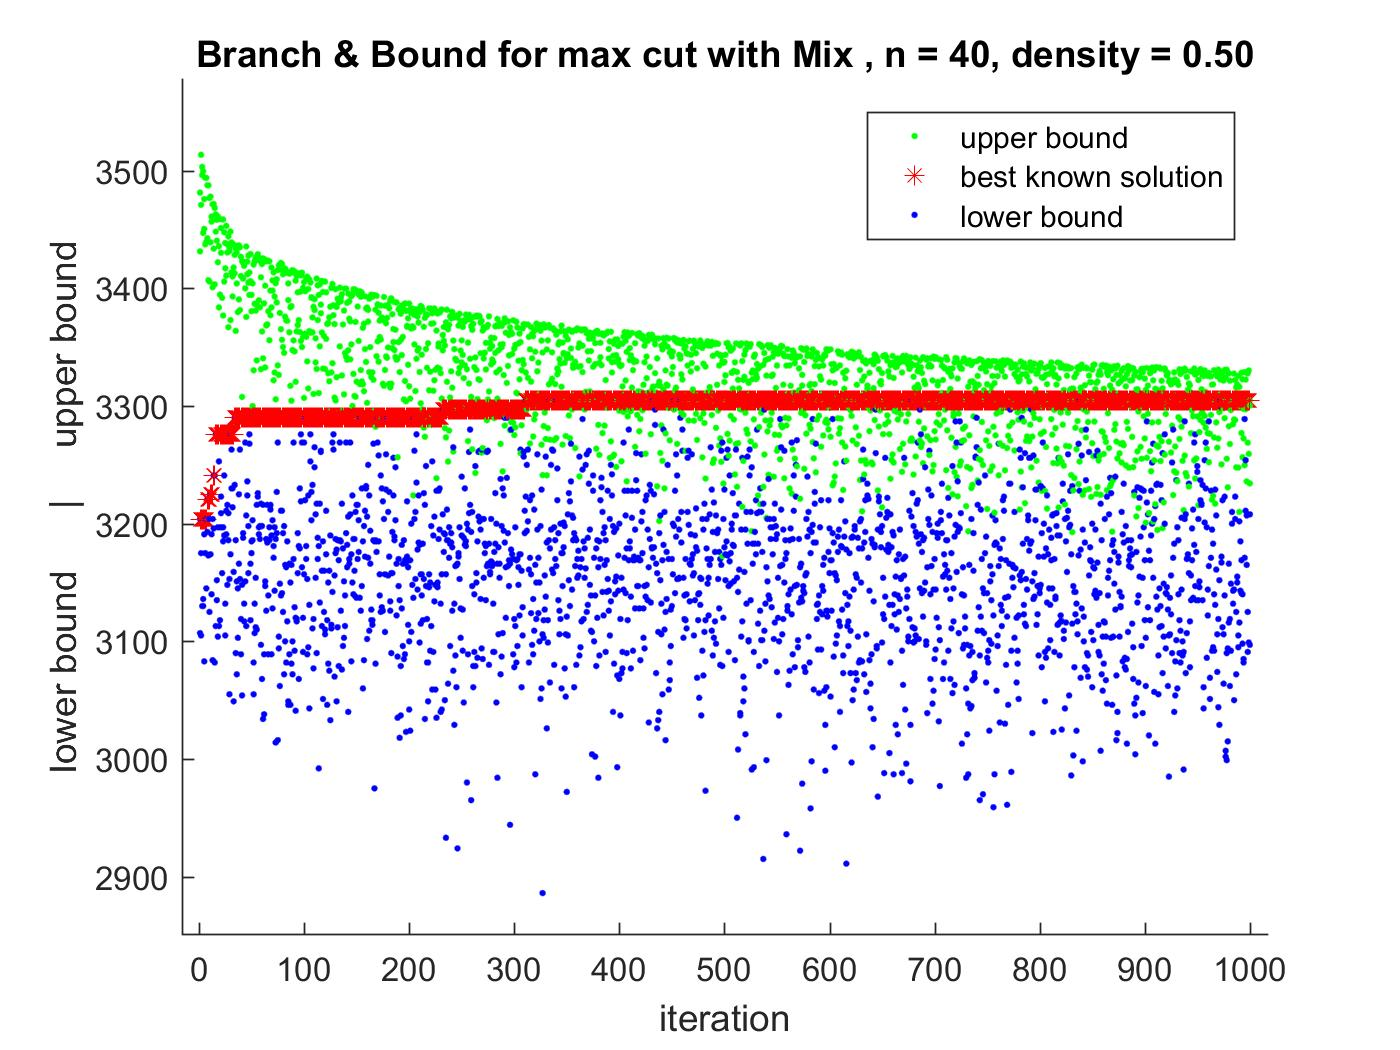
\includegraphics[scale=0.27]{img/bnb_mix_n40_d50_1.jpg}
\caption[Branch and bound for mixed SOCP-SDP relaxation]{Branch and bound for mixed SOCP-SDP relaxation. }
\label{FigureBnb1mix}

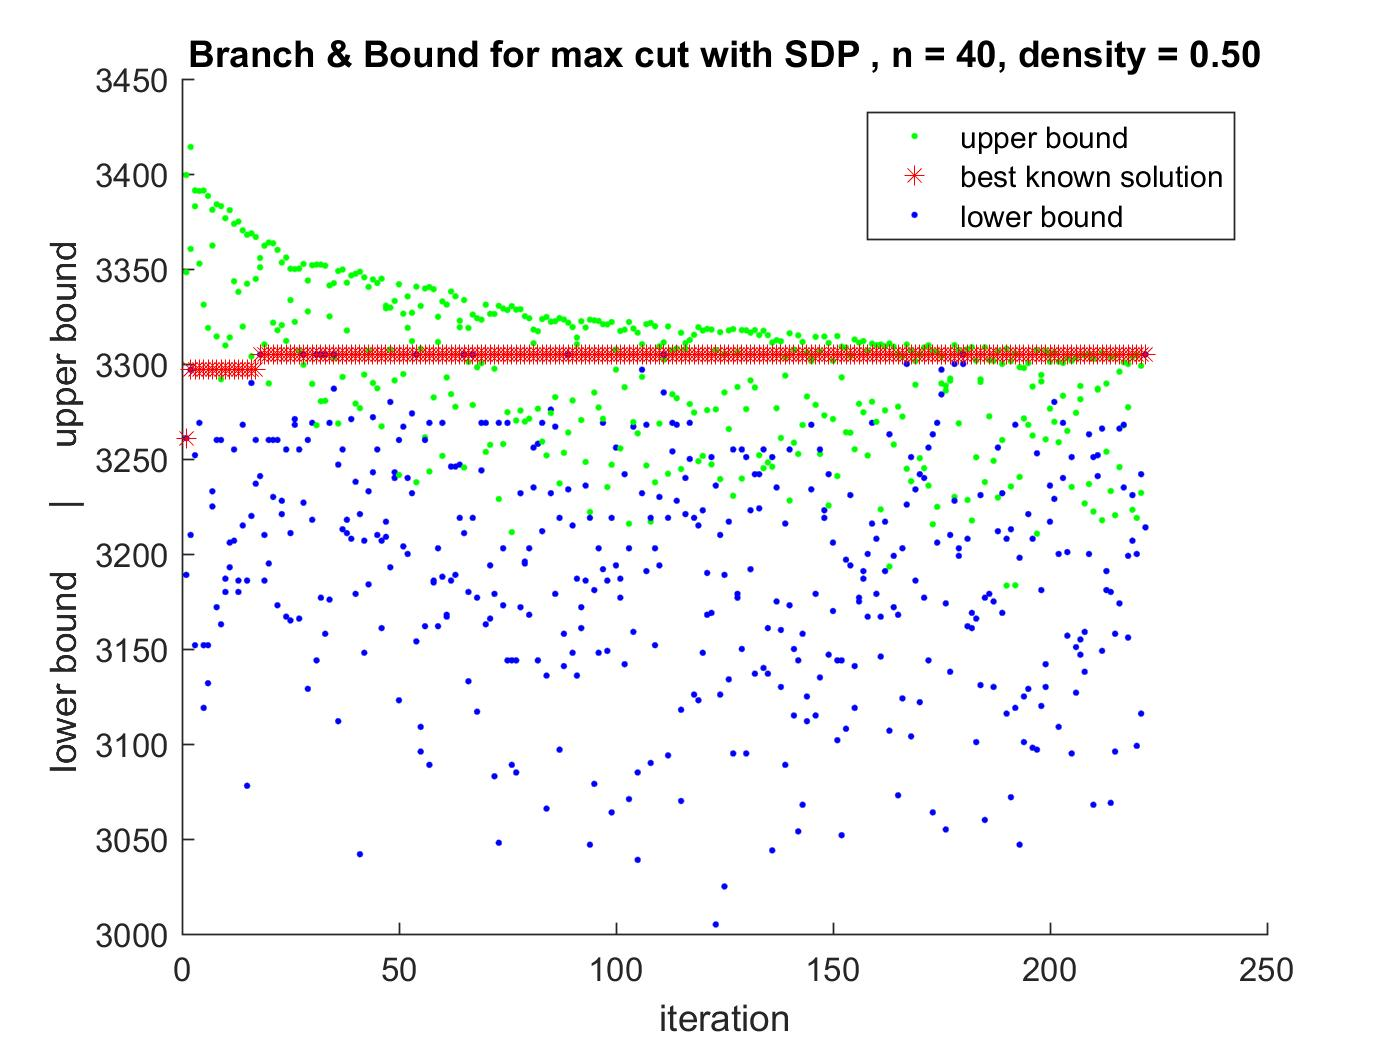
\includegraphics[scale=0.27]{img/bnb_sdp_n40_d50_1.jpg}
\caption[Branch and bound for SDP relaxation]{Branch and bound for SDP relaxation. }
\label{Figurebnb1sdp}
\end{figure}


\subsection{Large scale instances}

In this section we are going to compare only fast methods (sdp, lp1, lp3, mix1, mix2 and  mixr for $r=50,20,10,5$) to see how the performance changes when problems grow large $n=100, 200, \dots ,600$.

For this comparison (in the Figures \ref{comp3}, \ref{comp3size}) we did not know the optimal values (it would be almost impossible for us to compute them), hence, we have approximated the relative errors as relative errors against the best obtained bound, which was for each instance the bound produced by SDP relaxation. We will prove later that this relation always holds for SDP and mixed SOCP-SDP relaxation.

In the Figure \ref{comp3} one can see that from the mixed methods the best bounds are produced by mix2 relaxation which has also one of the shortest run times. 


We offer also a problem-size breakdown of this experiment in the Figure \ref{comp3size} where it is clear that mix2 is superior for all sizes of problems. Moreover, that for all of the methods have more-less stable quality of the bounds and increasing run time for growing $n$.


% Comparing the different densities, we saw that relative error is a little higher for the sparse instances. It may be caused by the improved quality of sdp bounds for sparse instances. 
 



\subsection{Relation of Mix and SDP}

In the following, we would like to demonstrate that these mixed SOCP-SDP relaxations are for max-cut never stronger then SDP relaxation. 

Let $L = L^- + L^+$ be a splitting of $L$ with $L^-\preceq 0.$
We will consider a general mixed SOCP-SDP relaxation of (\ref{maxcut3}).
\begin{equation}
\label{MaxCutMixedRelaxGeneral}
\begin{array}{ll}
\mbox{maximize} & \frac{1}{4}\left[ X_1^TL^-X_1 + L^+\bullet X \right], \\
\mbox{subject to} &  diag(X) = e, \\
			& X\succeq 0,
\end{array}
\end{equation}
where $X_1$ denotes first column of $X$. We will refer to this problem as MIX.

\rem Notice that all of the mixed methods (mix1, mix2, mixr for any $r$) are included in this formulation for a certain choice of splitting $L^+, L^-$. Using the fact that $L^+\bullet X$ reduces to $Tr(L^+)$ when $L^+$ is diagonal yields an equivalent formulation.



\thm Consider an instance of QCQP \ref{qcqp}. Denote $\nu(SDP), \ \nu(Mix)$ the optimal values of the SDP relaxation (\ref{MaxCutSDPRelax}) and mixed SOCP-SDP relaxation MIX (\ref{MaxCutMixedRelaxGeneral}) respectively. It holds that $\nu(SDP)\leq \nu(MIX)$.
\rm
\begin{proof}
Notice, that both relaxations have same feasible set $F = \{X\in \mathbb{S}^n \ \vert \ diag(x) = e,\ X\succeq 0.\}$. We will show that for any $X\in F$ the objective value of SDP is at most the objective value of MIX. Indeed
\begin{equation}
\label{ProofRelationMixSDP}
\begin{array}{rcl}
L\bullet X - ( X_1^TL^-X_1 + L^+\bullet X) 
& = & L^-\bullet X - X_1^TL^-X_1 \\ 
&=&  L^-\bullet (X - X_1 X_1^T) \\ 
&\leq & 0.
\end{array}
\end{equation}
The inequality hods because $L^-\preceq 0$ and $X-X_1X_1^T\succeq 0$,
since from $X\succeq 0$, using that$X_{11}=1$, $X_1$ is the first column of $X$ and Schur complement lemma (see \ref{SchurCompl} in the Appendix) we have $X\succeq X_1X_1^T.$ 
\end{proof}

\rem Using the difference (\ref{ProofRelationMixSDP}) expressed in he previous proof, we can bound a a difference of $\nu(MIX)-\nu(SDP)$ in tho following way. Let $\hat{X}, \hat{X}_1$ be the optimal solution of MIX with the objective $\nu(MIX)$. Then $\hat{X}$ is also a feasible solution of SDP with the objective $\nu_{SDP}(\hat{X})$ such that
$$\nu(MIX)\geq \nu(SDP) \geq \nu_{SDP}(\hat{X})\geq \nu(MIX) + \frac{1}{4}L^-\bullet (\hat{X} - \hat{X}_1 \hat{X}_1^T).$$
Hence, if $\vert L^-\bullet (\hat{X} - \hat{X}_1 \hat{X}_1^T)\vert$ is small, the the bound of MIX is guaranteed to be very close to bound produced by SDP. 






\section{Branch and bound}
\label{SectionBranchAndBound}



We will first describe the general idea of the branch and bound algorithms.  Suppose we are dealing with a minimization problem.

The basic idea of this method is to divide and conquer. There are 3 basics steps we will do repeatedly. Branch, compute bounds and prune.

\textbf{Branch.} First divide by branching the original problem into the smaller subproblems i.e. by partitioning the feasible set. 
 In combinatorial (discrete) problems this can be done by fixing a variable. For example if $x_l \in \{0,1\}$, then by fixing $x_l=1$ and $x_l=0$ respectively, the problem is divided into two subproblems with one less free variable $x_{-l} \in \{0,1\}^n.$


\textbf{Compute bounds.} The lower bounds should be established for each branch. Usually this is done by solving the relaxed problem for each subproblem. 
An upper bound is computed on the optimal value, this can be done by finding a feasible solution for a chosen subproblem. It is often extracted from the solution of the relaxed problem using a projection or a rounding procedure.

\textbf{Prune.} Having both lower and upper bounds, conquer by pruning all the branches with lower bound greater then global upper bound. The optimal solution is surely not in these branches.

\textbf{Repeat.} This process is repeated by branching the remaining subproblems, computing the new (better) lower bounds for these smaller problems, improving the upper bound and further pruning the problem tree.

One can use more or less clever techniques to decide when, how and which subproblems to branch or how and when to compute bounds.
Using stronger relaxations for bounding steps results in increased computation time, but hopefully less iterations are needed since better bounds allow to cut branches earlier.  On the other hand weaker relaxations are computed faster so they let us do more iterations and explore much greater portion of the problem tree. The greater number of iterations increases chances for guessing the optimal solution as well as obtaining good lower bounds for problems that are small enough.

\subsection{Our branch and bound framework}


\begin{table}
\centering
\begin{tabular}{|l|l|l|l|l|l|l|l|}\hline
\multicolumn{4}{|c|}{SDP} & \multicolumn{4}{|c|}{mix} \\ \hline 
opt  &  topIter  &  iter &  time &  opt  &  topIter &  iter 	 &  time    \\
\hline  \hline  

    3093    &     4      &       72    &     38.978   &   3093    &     4     &        371   &     241.51      \\      
    3342    &     3      &       70    &     44.229   &   3342    &     5     &        854   &     710.19      \\       
    3262    &     1      &      108    &     54.709   &   3262    &     4     &        723   &     493.06      \\    
    3330    &    54      &      130    &     69.598   &   3330    &    52     &       1000   &      750.6      \\    
    3279    &   130      &      171    &     107.22   &   3279    &     1     &       1306   &     1099.7      \\    
    3216    &   190      &      237    &     151.78   &   3216    &   947     &       1626   &     1387.1      \\    
    3293    &   143      &      175    &     117.01   &   3293    &   215     &       1155   &     976.52      \\    
    3335    &     4      &       44    &     29.234   &   3335    &     4     &        392   &     327.49      \\    
    3322    &    20      &      123    &     67.561   &   3322    &   409     &        764   &     506.83      \\    
    3382    &    44      &      117    &     75.352   &   3382    &   117     &        865   &     734.63      \\    
    2866    &   170      &      478    &     315.12   &   2861    &    90     &       3000   &     2535.4      \\  \hline 
\end{tabular}
\caption[Branch and bound comparison table]{Table of branch and bound solution instances for $n=40$, density $50\%$.
Columns: opt - optimal value or the best solution found, topIter - a number of iteration when opt was found, iter - total number of iterations, time - total time. A maxumum number of iterations was set to 3000 (the last instance of mix did not finish)}
\label{TableBnb}
\end{table}


%%%% tu boli obrazky

We will be branching the problem tree by fixing the variables $x_i$.
At the beginning the only fixed variable is $x_1=1$. This is without loss of generality, because if there is an optimal solution $\hat{x}$ then $-\hat{x}$ having the same objective value is also an optimal solution. 


\subsubsection{Problem formulations}
Each problem solved during the branch and bound procedure will be represented by sets of indices fixed to 1 and -1:  
$$P = \{i\in V \ \vert \ x_i =1 \ \mbox{is fixed} \}, \ \ \ \
N = \{i\in V \ \vert \ x_i =-1 \  \mbox{is fixed} \}, $$
with $P\cap N = \emptyset.$ 
Let us denote the set of known indices $K = P\cup N$ and set of unknown indices $U = V\setminus K$. 

%Suppose that only first $k$ vertices are fixed, i.e. $K = \{1,\dots ,k\}$. This is without loss of generality, since this can be achieved by renaming vertices. 

Now the objective $x^TLx/4$ of the problem (\ref{maxcut3}) with fixed indices reduces to 
\begin{eqnarray*}
\frac{1}{4}x^TLx &=& \frac{1}{4}(x_K^T , x_U^T )
\left(\begin{array}{rr} L_{KK} & L_{KU} \\ L_{KU} & L_{UU} \end{array}\right)\left(\begin{array}{c} x_K \\ x_U \end{array}\right) \\
&=& \frac{1}{4} \left[ x^T_UL_{UU}x_U +2x^T_KL_{KU}x_U + x^T_KL_{KK}x_K \right].
\end{eqnarray*}
The resulting problem of the size $n-k$ with variable $x_U\in\{0,1\}^n$ 
is 
\begin{equation*}
\begin{array}{ll}
\mbox{maximize } & \frac{1}{4} \left[ x^T_UL_{UU}x_U +2x^T_KL_{KU}x_U + x^T_KL_{KK}x_K \right], \\
\mbox{subject to } & x_U\in\{0,1\}^n.
\end{array}
\end{equation*}


It has following SDP relaxation 
\begin{equation*}
\begin{array}{ll}
\mbox{maximize } & \frac{1}{4} \left[ L_{UU}\bullet X_{UU} +2x^T_KL_{KU}x_U + x^T_KL_{KK}x_K \right], \\
\mbox{subject to } & diag(X_{UU}) = 1, \\
				& X_{UU}\succeq x_Ux_U^T.
\end{array}
\end{equation*}

And following mixed SOCP-SDP relaxation (mix2)
\begin{equation*}
\begin{array}{ll}
\mbox{maximize} & \frac{1}{4}\left[ \ x_U^T(\bar{D}_{LU} - \lambda_{max}(\bar{D}_{LU})I)x_U  + 2x^T_KL_{KU}x_U \ +  \ \right. \\
	& \left. \ \ \ + \ x^T_KL_{KK}x_K + e^TD_{LU} + \lambda_{max}(\bar{D}_{LU})(n-k)  \ \right], \\
\mbox{subject to} &  x_i^2 \leq 1, \ (i=1,\dots ,n),
\end{array}
\end{equation*}
where $D_{LU}$ is the $n-k\times n-k$ diagonal matrix  with diagonal entries of $L_{UU}$, $\bar{D}_{LU} = L_{UU} - D_{LU}$ is its complement and $\lambda_{max}(\bar{D}_{LU})$ denotes the largest positive eigenvalue of $\bar{D}_{LU}.$


\subsubsection{Branching}
For the branching we have tried many approaches, of which the most reasonable seemed to be fixing either vertices with large degrees (in the remaining graph) to sparsify the residual graph or the vertices with the greatest contribution to the scalar term $x_K^TL_{KK}x_K$ after being fixed.

Both of these approaches are heuristics, first one aims to simplify the graph, the second one tries to secure large part of the objective as soon as possible. That suggest a compromise of these may be a good idea. That is in each node we will randomly decide either with probability $p_{d}$ to branch by the degree and with probability $1-p_d$ to branch by the weight of contribution.

It seem that for dense graphs larger $p_d$ works better, on the other hand for sparse graphs, smaller $p_d$ gives better results.

\subsubsection{Producing lower bounds}
For the SDP relaxation we will use the rounding algorithm by Goemans and Williamson [\ref{GoemansWilliamsonMaxCut}] (see the Section \ref{SectionGoemansAndWIlliamson}). For the mixed relaxation we will use simple rounding of $x$ to $sign(x)$.

\rem We have tried to develop another rounding procedures for mix2. Specifically, we have considered creating a matrix $X\succeq 0$ with $diag(X) = e$ such that $x$ would be its first column, in order to use the GW-algorithm for SDP with guaranteed 0.878 performance. We tried to construct $X$ as a feasible soulution for SDP with objective as close to the objective of mix as possible. To keep the most information from $x$ a following structure of $X$ was expected
$X = xx^T + diag(u) + \bar{U}$, where $diag(\bar{U}) = 0$. The diagonal part is determined by requiring $diag(X) = e$. On the other hand, finding $\bar{U}$  such that difference of the objectives (\ref{ProofRelationMixSDP}) is minimal and $xx^T + diag(u) + \bar{U} = X \succeq 0$ is an SDP in variable $\bar{U}.$/

\subsubsection{Rounding upper bounds}
In our experiments we will only test instances with integer edge weights. Therefore, the optimal value is also expected to be integer. In our experiments we will always improve the upper bounds by rounding them down.
  


\subsection{Branch and bound comparison}
In this section we are going to comapre mix2 and sdp relaxations in th branch and bound procedure. In the table \ref{TableBnb} one can see that solving the max cut to optimality takes several times longer with mixed SOCP-SDP than with SDP bounds.
However, one can see that optimal solution is usually found quite soon. It is the proof of optimality that takes most of the time.

Before we have seen that differences in bounds are small in relative, but in the Figures \ref{FigureBnb1mix}, \ref{Figurebnb1sdp} it is clear those small relative differences are significant for proving the optimality.

Lastly the Figure \ref{Figurebnb3} shows how the branching procedure manages to exclude problems in time.

An interesting observation is that usually the optimum is found after a fraction of time needed to complete the BnB procedure. Therefore few iterations of BnB can be used to strengthen the relaxation. It can improve both the upper bound as a maximum of the upper bounds of all considered subproblems, and the lower bound as the best found feasible solution. One can use heuristics for ordering the subproblems in BnB with aim to focus more on the former (the high upper bounds are computed first) or the latter (branches where the best feasible solutions were found are explored first). This approach offers further flexibility in choosing the time-precision trade off of the relaxation techniques.




\chapter*{Conclusion}
\addcontentsline{toc}{chapter}{Conclusion}
\markboth{CONCLUSION}{}


This thesis surveyed the relaxation methods, mostly for QCQP. We introduced both well known approaches for constructing relaxations (such as LP and SDP relaxations), as well as approaches that are unfamiliar (SOCP and mixed relaxations) or recent (Lasserre hierarchy, DNN relaxations, CP and CPP reformulations). Throughout this thesis we discussed techniques for strengthening the relaxations gain the precision - adding valid inequalities (RLT, PSD-cuts, triangle inequalities for max-cut). But also techniques for decreasing the problem size and running time (SOCP and mixed SOCP-SDP relaxations, Lagrangian DNN primal-dual pair)

In the first chapter we gave organized introduction to conic programming classes showing key relations between them. We also highlighted their common structure by associating them with the general cone programming class. We have further used this class to derive dual problems for all conic classes at once.  

The second chapter offers extensive overview of relaxation techniques. We have gathered many approaches of relaxing the quadratic problems by conic optimization classes and arranged them systematically, showing the motivations for the techniques and providing links between them. 

In the third chapter we profoundly explore the application of the relaxation methods to the maximum cut problem. We formulate 16 relaxations, including their adaptations strengthened with valid inequalities.

These methods were compared by numerical experiments in the fourth chapter, which confirmed that SDP relaxation seems to be the most reasonable compromise, both in speed and quality of the produced bounds. In addition for a computational cost, SDP can be strengthened by valid inequalities. On the other hand, also the mixed SOCP-SDP methods proved to be reasonable compromise offering both quality bounds and exceptional time performance. 
At the end we suggest a possibility of using the branch and bound procedure for strengthening the relaxations. 

In the appendix we cover basic properties of cones and include examples showing the important properties of the cones used throughout the thesis. 

We believe that this thesis may serve as comprehensive guide through the field of relaxation methods for problems of quadratic programming.

 


\begin{appendix}	
%\addcontentsline{toc}{chapter}{A. \ \ Appendix}
%\renewcommand{\thechapter}{\Alph{chapter}}%
%\setcounter{chapter}{0}
\chapter[Appendix]{ }
\chaptermark{version for header}

\section{Schur complement}

We will first define the Moore-Penrose pseudoinverse which we will use in following theorem.
\defi[Moore-Penrose pseudoinverse]
\label{Pseudoinverse}
For a matrix $A\in\mathbb{R}^{m\times n}$ a pseudoinverse of $A$ is defined as a matrix $A^\dagger\in \mathbb{R}^{n\times n}$ satisfying all of the following
\begin{eqnarray*}
AA^\dagger A \ &=& A,\\
A^\dagger A A^\dagger &=& A,\\
(AA^\dagger)^T &=& AA^\dagger,\\
(A^\dagger A)^T &=& A^\dagger A.
\end{eqnarray*}

\thm[Schur complement lemma {[\ref{BoydCvxOpt}, \ref{ZhangSchurComplement}, \ref{GallierSchurCompl}]}] 
\label{SchurCompl}
Let $M$ be a symmetric matrix of the form
$$M = \left(\begin{array}{cc}
A & B\\
B^T & C
\end{array}\right).$$ 
Then $M\succeq 0$ ($M$ is positive semidefinite) if and only if 
$$A\succeq 0, \ \ \ \mathcal{R}(B)\subseteq \mathcal{R}(A),\ \ \ C - B^TA^\dagger B \succeq 0.$$


Where $A^\dagger$ denotes pseudoinverse of $A$ and $\mathcal{R}(B)$ denotes column range of $B$. (The roles of $A$ and $C$ can be switched.)\rm 

\proof A main idea of the proof is explained in [\ref{BoydCvxOpt}]. For a rigorous proof see any of [\ref{ZhangSchurComplement}, \ref{GallierSchurCompl}].


\section{Cones}
\label{Cones}
This Section is focused on providing introduction to the theory of cones and overview of basic claims and definitions.
Majority of the content in this section is from [\ref{PokornaSOCPDipl}]. At the end of this Section we provide examples dealing with cones $\mathbb{R}^n_+,\ \mathbb{Q}^n_+,\ \mathbb{S}^n_+, \ \mathbb{P}^n,\ \mathbb{C}^n,$  in order to prove all of the claims and properties used throughout this thesis.

\defi[Cone]
\label{defCone}
Set $\mathcal{K}$ is cone if for all $x\in \mathcal{K}$ and all $\theta\geq 0$, it holds that $\theta x \in \mathcal{K}$.



\defi[Proper cone] 
\label{defProperCone}
The cone $\mathcal{K}\subseteq \mathbb{R}^n$ is a proper cone if it has following properties
\begin{itemize}
\item $\mathcal{K}$ is closed
\item $\mathcal{K}$ is convex (for any $\theta_1,\theta_2\geq 0$ and $x_1,x_2\in\mathcal{K}$ also $\theta_1x_1 + \theta_2x_2 \in\mathcal{K}$)
\item $\mathcal{K}$ has nonempty interior  ($int \ \mathcal{K} \neq \emptyset$)
\item $\mathcal{K}$ is pointed (does not contain any line, i.e. if $\pm x\in \mathcal{K}$, then $x=0$).
\end{itemize}

\defi[Dual cone]
\label{defDualCone}
For any cone $\mathcal{K}$ we define its dual cone $\mathcal{K}^*$ as a set
\begin{equation*}
\mathcal{K}^* = \{z\ |\ \forall x\in\mathcal{K}, \ x^Tz\geq 0\}.
\end{equation*}
If  $\mathcal{K} =  \mathcal{K}^*$ we say cone $\mathcal{K}$ is selfdual.



%In the following section we will need to use the Separating hyperplane theorem.
%\thm[Separating hyperplane {[\ref{BoydCvxOpt}]}] 
%\label{SeparatingHyperplaneThm}
%Let $C\subseteq \mathbb{R}^n$ be a closed convex set and let $x_0\notin C$. 
%Then there exists $a \in \mathbb{R}^n$, $a\neq 0$ and $b\in \mathbb{R}$, such that 
%$a^Tx\geq b$ $\forall x\in C$ and $a^Tx_0<b$.
%\begin{proof}
%Since this theorem is well known, we only refer to proof in the literature see i.e. [\ref{BoydCvxOpt}]. 
%\end{proof}

\prop[{[\ref{PokornaSOCPDipl}]}] \label{DualConePropertiesProp}
Following holds for dual cone $\mathcal{K}^*$
\begin{enumerate}
\item  $\mathcal{K}^*$ is convex,
\item  $\mathcal{K}^*$ is closed,
\item if $int \ \mathcal{K}\neq \emptyset$ then $\mathcal{K}^*$ is pointed ,
\item if closure of $\mathcal{K}$ is pointed cone then $int \ \mathcal{K}^*\neq \emptyset$.
\end{enumerate}

\cor \label{DualOfAProperConeCorr}
If $\mathcal{K}$ is proper cone then also the dual cone $\mathcal{K}^*$ is proper.

\begin{proof}
\begin{enumerate}
\item Let $z_1,z_2 \in  \mathcal{K}^*$. Then from definition of dual cone, for any $\theta_1,\theta_2 \geq 0$ and $x \in \mathcal{K}$ it holds that
\begin{equation*}
x^T(\theta_1z_1 + \theta_2z_2) = \theta_1x^Tz_1 + \theta_2x^Tz_2 \geq 0,
\end{equation*}
which implies convexity of $\mathcal{K}^*$.% since $z_1,z_2$ were arbitrary points of $\mathcal{K}^*$.

\item Let $\{z_n\}_{n=1}^\infty$ be a convergent sequence of points in $\mathcal{K}^*$, such that 
$z_n\rightarrow z$. It is sufficient to show that $z\in \mathcal{K}^*.$  Indeed, for any $x\in \mathcal{K}$ and positive integer $n$ we have $x^Tz_n \geq 0$, therefore
$\lim_{n\rightarrow \infty} x^Tz_n = x^Tz \geq 0$. Hence $z\in \mathcal{K}^*.$

\item Let $int \ \mathcal{K}\neq \emptyset$. It suffices to prove that $\mathcal{K}^* \cap (-\mathcal{K}*) = \{0\}.$ Let $y\in \mathcal{K}^* \cap (-\mathcal{K}*)$, then 
$x^Ty = 0 $ for all $x\in \mathcal{K}$. Since $int \ \mathcal{K}\neq \emptyset$, there exist open ball $B\subset \mathcal{K}$. By contradiction, suppose that $y\neq 0$, then there is $u\in \mathbb{R}^n$ such that $y^Tu>0$. Now take any $x\in B$ and $\alpha>0$ such that $x+\alpha u\in B$, we have 
$$ 0 = y^T(x+\alpha u) = y^Tx + \alpha y^Tu = 0 + \alpha y^Tu > 0,$$
and that is a contradiction.


\item Denote $\bar{\mathcal{K}}$ the closure of $\mathcal{K}$ and let $\bar{\mathcal{K}}$ be pointed, i.e. 
$\bar{\mathcal{K}} \cap \left(-\bar{\mathcal{K}}\right) = \{0\}$. First, we will show that $0\notin conv(S^n\cap \bar{\mathcal{K}}).$ By contradiction, if $0\in conv(S^n\cap \bar{\mathcal{K}})$ then there are some 
$x^1,\dots ,x^m \in \left(S^n\cap \bar{\mathcal{K}}\right)$ and 
$\theta_1,\dots \theta_m \geq 0$, such that $\sum_{i=1}^m = 1$ and $ 0 = \sum_{i=1}^m \theta_ix^i$.
Let $j$ be an index for which $\theta_j\neq 0$ (there must be at least one such index). Then 
\begin{equation*}
\theta_jx^j \in \bar{\mathcal{K}} \ \mbox{ and } \ -\theta_jx^j= \sum_{i\neq j} \theta_ix^i \in \bar{\mathcal{K}}.
\end{equation*}
This is a contradiction, because  $\bar{\mathcal{K}}$ is pointed, hence $0\notin conv(S^n\cap \bar{\mathcal{K}}).$
Since $conv(S^n\cap \bar{\mathcal{K}})$ is closed and convex, by separating hyperplane theorem (see [\ref{BoydCvxOpt}]) there exists nonzero $a\in \mathbb{R}^n$ and $b\in \mathbb{R}$ such that 
$a^Tx \geq b$ for any $x\in (S^n\cap \bar{\mathcal{K}})$ and $a^T0<b$. Therefore $b>0$ and for any nonzero $y\in  \bar{\mathcal{K}}$, since the $y/\Vert y\Vert \in (S^n\cap \bar{\mathcal{K}})$
we have 
$$a^Ty = \Vert y \Vert a^T \frac{y}{\Vert y\Vert} \geq \Vert y\Vert b > 0,$$
hence $a\in \mathcal{K}^*$.  

We will show that the ball with center $a$ and radius $b$ ($B(a,b)$) is contained in $\mathcal{K}^*$, hence $a\in int \ \mathcal{K}^*$. Take arbitrary $u\in \mathbb{R}^n$, such that $\Vert u \Vert <b$. From Cauchy-Schwartz inequality we have
$$u^Ty \geq - \vert u^Ty \vert \geq -\Vert u \Vert \Vert y \Vert, \ \mbox{ i.e. } \ u^Ty/\Vert y \Vert \geq -\Vert u \Vert.$$ Now 
$$ (a+u)^Ty = a^Ty + u^Ty \geq b\Vert y \Vert - \Vert u \Vert \Vert y \Vert = (b - \Vert u \Vert)\Vert y \Vert\geq 0.$$
Therefore $a\in int\ \mathcal{K}^* \neq \emptyset$ and proof is complete.

\end{enumerate}
\end{proof}

\prop \label{PropSecondDualofClosedCOne} If $\mathcal{K}$ is closed convex cone then $\mathcal{K}^{**} = \mathcal{K}$.

\begin{proof}
Recall that 
$$ z \in \mathcal{K}^{**} \ \Leftrightarrow \  y^Tz \geq 0 \ \forall y\in \mathcal{K}^{*}.$$
The inclusion $\mathcal{K} \subseteq \mathcal{K}^{**}$ follows directly from the definition of $\mathcal{K}^{*}$, since $y\in\mathcal{K}^{*}$ if and only if $x^Ty\geq 0$ for all $x\in \mathcal{K}$. 

Next we will show the second inclusion  $\mathcal{K}^{**} \subseteq \mathcal{K}$ by contradiction.
Suppose that there is $z \in \mathcal{K}^{**}$ with $z \notin \mathcal{K}$.
Since $\mathcal{K}$ is closed and convex, there is a hyperplane separating $z$ and $\mathcal{K}$ (see [\ref{BoydCvxOpt}]), i.e. there is an $a \in \mathbb{R}^n, $ such that 
$$ a^Tz <0  \ \mbox{ and } \ a^Tx\geq 0, \ \forall x\in\mathcal{K}.$$
The second inequality implies that $a\in \mathcal{K}^*$, but then  $ a^Tz <0 $ contradicts $z\in \mathcal{K}^{**}$.

All in all,  we have $\mathcal{K}^{**} = \mathcal{K}$.
\end{proof}



%
%\prop[{[\ref{PokornaSOCPDipl}]}] 
%\label{ConesCartesianProduct}
%Let $\mathcal{K} = \mathcal{K}_1 \times \cdots \times \mathcal{K}_m $ be a Cartesian product of cones. Then
%\begin{enumerate}
%\item $\mathcal{K}$ is a cone.
%\item If $\mathcal{K}_1, \cdots ,\mathcal{K}_m $ are convex cones, then $\mathcal{K}$ is convex.
%\item If $\mathcal{K}_1, \cdots ,\mathcal{K}_m $ are selfdual cones, then $\mathcal{K}$ is selfdual.
%\item If $\mathcal{K}_1, \cdots ,\mathcal{K}_m $ are proper cones, then $\mathcal{K}$ is proper.
%\end{enumerate} 
%\begin{proof}
%See [\ref{PokornaSOCPDipl}].
%\end{proof}
%
%
%


%TODO Figures

\section{Examples}


\ex[Closed convex cones] The following sets are closed convex cones 
\label{ExClosedConvexCones}
\begin{enumerate}
\item Nonnegative orthant $\mathbb{R}^n_+$,
\item Nonnegative cone $$\mathbb{N}^n = \{M\in \mathbb{R}^{n\times n} \ \vert \ M_{ij} \geq 0, \ \forall i,j=1,\dots ,n\},$$
\item Second order cone $$\mathbb{Q}^n=\{x\in \mathbb{R}^n \ | \ x = (x_0,\bar{x}) \in \mathbb{R}\times\mathbb{R}^{n-1}, \|\bar{x}\|_2\leq x_0\},$$
\item Set of symmetric positive semidefinite matrices  $$\mathbb{S}^n_+ = \{M \in \mathbb{S}^n \ \vert \ x^TMx\geq 0, \  \forall x\in \mathbb{R}^n\},$$
\item Set of copositive matrices $$\mathbb{C}^n = \{M \in \mathbb{S}^n \ \vert \ x^TMx\geq 0, \  \forall x\in \mathbb{R}^n_+\},$$
\item Set of completely positive matrices $$\mathbb{P}^n = \{M\in \mathbb{S}^n \ | \ M = \sum_{i = 1}^l x^{i}x^{iT} \ \mbox{ where } x^i \in \mathbb{R}^n_+ \ (i = 1,\dots ,n) \}.$$
\end{enumerate} 

%\begin{proof}[Proof version 1]
%All the parts follow straightforward from the definition. 
%\end{proof}
\begin{proof}%[Proof version 2]
The fact that each of the sets is closed is simple since all of them are defined only using nonstrict inequalities (and symmetry), which will also hold in limit. % of a sequence of points 
\begin{enumerate}
\item[1. -- 2.] Follows simply from the definition.
\setcounter{enumi}{2}
\item (It is a cone). Let $(x_0,\bar{x})= x\in \mathbb{Q}^n$ and $\theta \in \mathbb{R}^n_+$.
Then for $\theta x = (\theta x_0, \theta\bar{x})$ we have  
$$\Vert \theta\bar{x}\Vert_2 = \theta \Vert \bar{x}\Vert_2 \leq \theta x_0.$$

(It is convex). Let $x=(x_0,\bar{x}),y=(y_0,\bar{y})\in\mathbb{Q}^n$ and $\theta_1, \theta_2 \geq 0$.
Then 
\begin{eqnarray*}
\theta_1x + \theta_2y &=& (\theta_1x_0+\theta_2y_0,\  \theta_1\bar{x} + \theta_2\bar{y}),  \\
\Vert \theta_1\bar{x} + \theta_2\bar{y} \Vert_2 &\leq & \Vert \theta_1\bar{x} \Vert_2 + \Vert \theta_2\bar{y} \Vert_2 \leq  \theta_1x_0+\theta_2y_0.
\end{eqnarray*}

\item (It is a cone) Let $M\in \mathbb{S}^n_+$, that is $x^TMx\geq 0$ $\forall x\in\mathbb{R}^n$ and $\theta \geq 0$. Then $$x^T(\theta M)x = \theta(x^TMx) \geq 0 \ \forall x\in\mathbb{R}^n \ \Leftrightarrow \ (\theta M) \in \mathbb{S}^n_+.$$

(It is convex)  Let $M_1, M_2\in \mathbb{S}^n_+$, and $\theta_1, \theta_2 \geq 0$. Then
$$x^T(\theta_1M_1 + \theta_2M_2)x = x^T\theta_1M_1x + x^T\theta_2M_2x \geq 0 \ \forall x\in\mathbb{R}^n \ \Leftrightarrow \ (\theta_1M_1 + \theta_2M_2) \in \mathbb{S}^n_+.$$

\item Analogically as for $\mathbb{S}^n_+$, only $\mathbb{R}^n$ is replaced by $\mathbb{R}^n_+$.

\item (It is a cone) Let $M\in \mathbb{P}^n$ and $\theta \geq 0$. Since $M$ is completely positive, there are nonnegative vectors $x^i$, $i = 1,\dots , l$ such that
$$ \theta M = \theta\sum_{i = 1}^l x^{i}x^{iT} = \sum_{i = 1}^l (\sqrt{\theta} x^{i})(\sqrt{\theta} x^{i})^T.$$

(It is convex) Let $M_1, M_2\in \mathbb{P}^n$ and $\theta_1, \theta_2 \geq 0$. Since $M_1, M_2$ are completely positive, there are nonnegative vectors $x^i, y^j$, ($i = 1,\dots , l_1$ and $j = 1,\dots ,l_2$)  such that
\begin{eqnarray*}
 \theta_1 M_1 + \theta_2 M_2 &=& \theta_1\sum_{i = 1}^{l_1} x^{i}x^{iT} + \theta_2\sum_{j = 1}^{l_2} y^{j}y^{jT} \\
 		& = & \sum_{i = 1}^{l_1} (\sqrt{\theta_1} x^{i})(\sqrt{\theta_1} x^{i})^T + \sum_{j = 1}^{l_2} (\sqrt{\theta_2} y^{i})(\sqrt{\theta_2} y^{i})^T .
\end{eqnarray*}
\end{enumerate}
\end{proof}

%\begin{figure}
%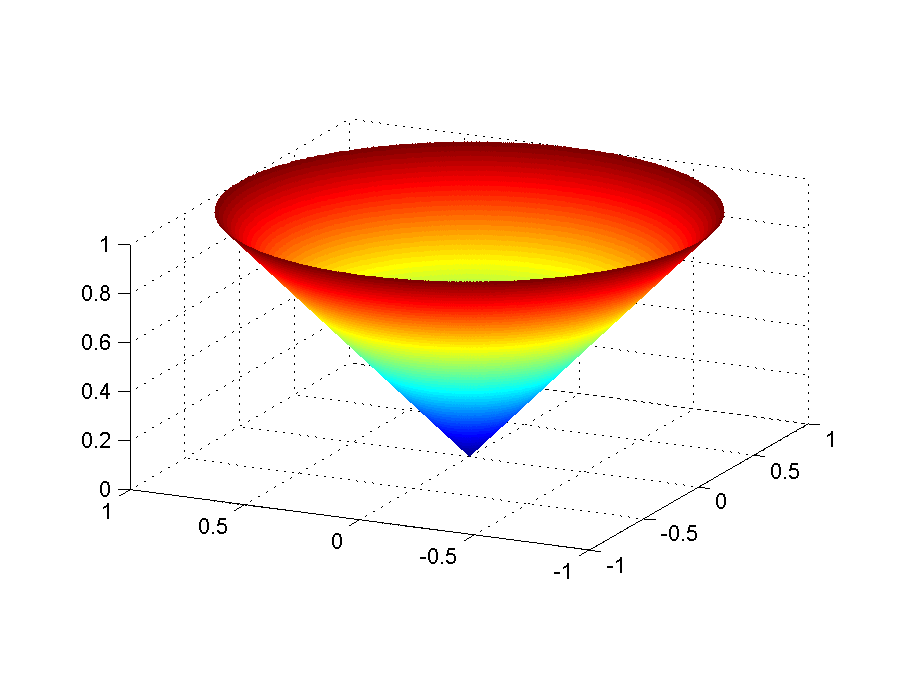
\includegraphics[scale=1]{img/soc.eps}
%\caption[Second order cone in $\mathbb{R}^3$]{Second order cone in $\mathbb{R}^3$}
%\end{figure}
%
%\begin{figure}
%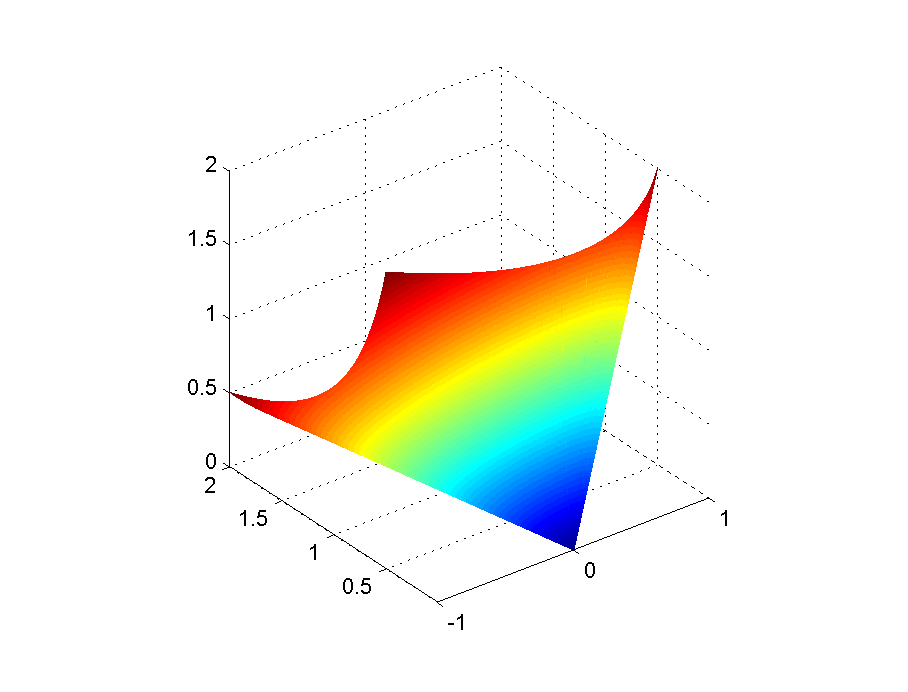
\includegraphics[scale=1]{img/sdcone1.eps}
%\caption[Semidefinite cone $\mathbb{S}^2_+$]{Semidefinite cone $\mathbb{S}^2_+$}
%\end{figure}


\ex[Proper cones] Following cones are proper
\label{ExProperCones}

\begin{enumerate*}
\item $\mathbb{R}^n_+$ , \ \
\item $\mathbb{N}^n$ , \ \
\item $\mathbb{Q}^n$ , \ \
\item $\mathbb{S}^n_+$ , \ \ 
\item $\mathbb{C}^n$ , \ \ 
\item $\mathbb{P}^n$ . \ \ 
\end{enumerate*}

\begin{proof} Since we have shown that all of them are closed convex cones (see Example \ref{ExClosedConvexCones}), we only need to prove that they are pointed and have nonempty interiors.
The first three cases are obviously pointed and have interior points (for example all ones vector for $\mathbb{R}^n_+$ and $(2,0^T)$ for $\mathbb{Q}^n$ are interior points - an open unit ball with these centres belongs to these cones). 
\begin{enumerate}
\setcounter{enumi}{3}
\item If positive semidefinite matrix $M$ is nonzero, it has at leas one positive eigenvalue $\lambda >0$ and corresponding eigenvector $u$ such that $u^TMu>0$. But then $u^T(-M)u = - u^TMu<0$, so $-M$ is not in $\mathbb{S}^n_+$ and therefore it is pointed. Any positive definite matrix is an interior point of $\mathbb{S}^n_+$, so it has nonempty interior. 

\item The $\mathbb{C}^n$ is closed, convex cone (see Example \ref{ExClosedConvexCones}). It is also easy to see that $\mathbb{C}^n$ has nonempty interior, since it contains $\mathbb{S}^n_+$ (which is proper).

We only need to show that $\mathbb{C}^n$ is pointed. For $M\neq 0$, $M\in\mathbb{C}^n\cap (-\mathbb{C}^n)$, 
then $x^TMx\geq 0$ and $x^T(-M)x\geq 0$ for all $x\in\mathbb{R}^n_+$, implying that 
$x^TMx=0$ for all $x\in\mathbb{R}^n_+$. Since any vector $v\in \mathbb{R}^n$ can be written as $v = x - y$ for some $x,y\in\mathbb{R}^n_+$ it also holds that $v^TMv=0$ for all $v\in\mathbb{R}^n$, hence $M=0$.

Therefore $\mathbb{C}^n$ is a proper cone. 

\item From the Corrolary \ref{DualOfAProperConeCorr} since $\mathbb{C}^n$ is a proper cone, its dual $\mathbb{P}^n$ is also proper.
\end{enumerate}
\end{proof}

\ex[Dual cones] The following properties about dual cones holds
\label{ExDualCones}
\begin{enumerate}
\item $\mathbb{R}^n_+$ is a selfdual cone,
\item $\mathbb{N}^n_+$ is a selfdual cone,
\item $\mathbb{Q}^n$ is a selfdual cone,
\item $\mathbb{S}^n_+$ is a selfdual cone,
\item $(\mathbb{C}^n)^* = \mathbb{P}^{n}$ \ and \ $(\mathbb{P}^n)^* = \mathbb{C}^{n}$, 
\item $(\mathbb{S}^n_+\cap \mathbb{N}^n)^* = \mathbb{S}^n_+ + \mathbb{N}^n$.
\end{enumerate}

\begin{proof}[Proof. \ ]
\begin{enumerate}
\item[\ 1. -- 2.] This is an easy observation.
\setcounter{enumi}{2}
\item Recall that $y\in(\mathbb{Q}^n)^*$ if and only if $x^Ty \geq 0$ for all $x\in\mathbb{Q}^n$. First we will show that $\mathbb{Q}^n \subseteq (\mathbb{Q}^n)^*$. For any $x = (x_0,\bar{x}),y=(y_0,\bar{y})\in \mathbb{Q}^n $ it holds that
$$ x^Ty = x_0y_0 + \bar{x}^T\bar{y} \geq \Vert \bar{x}\Vert_2 \Vert \bar{y}\Vert_2 - \vert \bar{x}^T\bar{y}\vert \geq 0,$$ where the first inequality holds from $x_0\geq \Vert \bar{x}\Vert_2$,  $y_0\geq \Vert \bar{y}\Vert_2$ and the second inequality follows from Cauchy-Schwartz inequality.

Now $(\mathbb{Q}^n)^* \subseteq \mathbb{Q}^n.$ Let $y\notin \mathbb{Q}^n$, we will show that $y\notin (\mathbb{Q}^n)^*$.
For such $y = (y_0,\bar{y})$ it holds that $y_0<\Vert \bar{y}\Vert_2$. Let $x = (\Vert \bar{y}\Vert_2, -\bar{y}),$ 
this $x$ belongs to $\mathbb{Q}^n$, but $x^Ty = \Vert \bar{y}\Vert_2(y_0-\Vert \bar{y}\Vert_2)<0$. So $y\notin (\mathbb{Q}^n)^*$ and we are done.

\item Recall that $M \in (\mathbb{S}^n_+)^*$ if and only if $P\bullet M \geq 0$ for all $P\in \mathbb{S}^n_+$. First we will first show that $\mathbb{S}^n_+ \subseteq (\mathbb{S}^n_+)^*$. For any $M,P\in \mathbb{S}^n_+$ it holds that 
$$P\bullet M = Tr(PM) = \sum_{i=1}^n \lambda_iu_i^TMu_i \geq 0,$$
where $\lambda_i\geq 0$, $u_i$  $(i=1,\dots ,n)$, are eigenvalues and eigenvectors of $P$.

Not the other inclusion. Let $M\notin \mathbb{S}^n_+$ be a symmetric $n\times n$ matrix, we will show that $M\notin (\mathbb{S}^n_+)^*.$ Since $M$ is not positive semidefinite, it has a negative eigenvalue $\lambda$ and corresponding eigenvector $u$. Then matrix $uu^T\in \mathbb{S}^n_+$ excludes $M$ from $(\mathbb{S}^n_+)^*$ since $uu^T\bullet M = u^TMu = \lambda <0$.

Therefore $\mathbb{S}^n_+ = (\mathbb{S}^n_+)^*$

\item First we will show $(\mathbb{P}^n)^* = \mathbb{C}^n$. From the definition, using the inner product $Tr(M^TP) = M \bullet P,$ we have
$$ (\mathbb{P}^n)^* = \{ M \in \mathbb{S}^n \ \vert \ M\bullet P\geq 0, \ \forall P\in \mathbb{P}^n \}. $$

Observe that for any $C\in \mathbb{C}^n$ and $P = \in \mathbb{P}^n,$ $P = \sum x^ix^{iT}$ it holds that 
$$ C\bullet P = \sum C\bullet x^ix^{iT} = \sum x^{iT}Cx^i \geq 0.$$
This implies $\mathbb{C}^n\subseteq (\mathbb{P}^n)^*$.

To prove the other inclusion $(\mathbb{P}^n)^* \subseteq \mathbb{C}^n$, take any $M\notin \mathbb{C}^n$. We will show that $M$ is neither in $(\mathbb{P}^n)^*$. For such $M$, there is a $x\in\mathbb{R}^n_+$, such that $x^TMx<0$. Indeed, the $xx^T \in \mathbb{P}^n$ then excludes $M$ from $(\mathbb{P}^n)^*$ since $M\bullet xx^T = x^TMx<0.$

We have proven that $(\mathbb{P}^n)^* = \mathbb{C}^n$. Since $\mathbb{P}^n$ is a closed convex cone, it holds that $\mathbb{P}^n = (\mathbb{P}^n)^{**} = ((\mathbb{P}^n)^{*})^* = (\mathbb{C}^n)^*$, and the proof is complete.

\item By definition 
$$(\mathbb{S}^n_+\cap \mathbb{N}^n)^* = \{ M\in\mathbb{S}^n \ \vert \ S\bullet M\geq 0, \forall S\in (\mathbb{S}^n_+\cap \mathbb{N}^n)\}. $$
Since both $\mathbb{S}^n_+,\ \mathbb{N}^n$ are selfdual, it is clear that $(\mathbb{S}^n_+ +\mathbb{N}^n) \subset (\mathbb{S}^n_+\cap \mathbb{N}^n)^*.$ Next also it is easy to see that 
\begin{equation}
\label{ExConesProofRelation1}
(\mathbb{S}^n_+ +\mathbb{N}^n)^* \subset (\mathbb{S}^n_+\cap \mathbb{N}^n),
\end{equation}
because 
when $M\notin \mathbb{S}^n_+$  then there is $S\in\mathbb{S}^n_+$ such that $M\bullet S < 0$. Also if $M\notin \mathbb{N}^n$ then there is $S\in\mathbb{N}^n$ such that $M\bullet S < 0$. So whe $M\notin (\mathbb{S}^n_+\cap \mathbb{N}^n)$ there is a matrix $S\in (\mathbb{S}^n_+ + \mathbb{N}^n)$ such that $S\bullet M <0$, excluding $M$ from $(\mathbb{S}^n_+ +\mathbb{N}^n)^*$.



For any cones $K_1\subset K_2$ it holds that $K_2^*\subset K_1^*$, therefore from (\ref{ExConesProofRelation1}) we have $$(\mathbb{S}^n_+ \cap \mathbb{N}^n)^* \subset (\mathbb{S}^n_+ + \mathbb{N}^n)^{**} = (\mathbb{S}^n_+ + \mathbb{N}^n).$$
The last equality holds from Proposition \ref{PropSecondDualofClosedCOne}, because $(\mathbb{S}^n_+ + \mathbb{N}^n)$ is closed cone. Thus we have proven both inclusions.
\end{enumerate}
\end{proof}
\end{appendix}

\chapter*{References}
\addcontentsline{toc}{chapter}{References}

\begin{enumerate}
\renewcommand*\labelenumi{[\theenumi]}




%%%%%% General
%
\item S. Boyd, L. Vandenberghe, \it Convex Optimization. \rm Cambridge University Press 2004, ISBN 978-0-521-83378-3, seventh printing with corrections, 2009 
%\\ \url{http://web.stanford.edu/~boyd/cvxbook/bv_cvxbook.pdf}
\label{BoydCvxOpt}
%
\item L. Tuncel, \it  Polyhedral and Semidefinite Programming Methods in Combinatorial Optimization. \rm  Fields Institute Monograph Series, AMS, Vol.FIM-27, 2010
\label{FieldsMono}
%
\item L. El Ghaoui, \it Introduction to Convex Optimization. \rm
A course EE 227A website on UC Berkeley, Available online: 
\url{https://inst.eecs.berkeley.edu/~ee227a/fa10/login/index.html}
\label{IntroToCvxOptBerkley}



%%%%%%% SDP
%\item R. M. Freund, \it Introduction to Semidefinite Programming (SDP), \rm 2009 \\ \url{http://ocw.mit.edu/courses/electrical-engineering-and-computer-science/6-251j-introduction-to-mathematical-programming-fall-2009/readings/MIT6_251JF09_SDP.pdf}
%\label{FreundIntroSDP}
%%
\item H. Wolkowicz, R. Saigal, L. Vandenberghe, \it Handbook of Semidefinite Programming: Theory, Algorithms, and Applications. \rm
ISBN 978-1-4615-4381-7, second printing, 2003
\label{HandbookSDP}
%



%%%%%%% SOCP
\item S. Burer, S.Kim, M. Kojima, \it Faster, but Weaker, Relaxations for Quadratically Constrained Quadratic Programs. \rm Computational Optimization and Applications, Vol.59 (1), pp 27-45, 2014
% \url{http://www.is.titech.ac.jp/~kojima/articles/socpsdp.pdf}
\label{BurerKimKojimaFasterWeakerRelax}
%
\item S. Kim, M. Kojima, \it Exact Solutions of Some Nonconvex Quadratic Optimization Problems via SDP and SOCP Relaxations.\rm  Computational Optimization and Applications, Vol.26 (2), pp 143-154, 2003
%\\ \url{http://www.is.titech.ac.jp/research/research-report/B/B-375.ps.gz}
\label{KimKojimaExactSolViaSDPandSOCP}
%
\item S. Kim, M. Kojima, \it Second Order Cone Programming Relaxations of Nonconvex Quadratic Optimization Problems. \rm Optimization Methods and Software, Vol.15 (3-4), pp 201-224, 2001 
%\\ \url{http://www.researchgate.net/publication/2637515_Second_Order_Cone_Programming_Relaxation_of_Nonconvex_Quadratic_Optimization_Problems}
\label{KimKojimaSOCPofNoncvxQOP}
%
\item S. Kim, M. Kojima, M. Yamashita, \it Second Order Cone Programming Relaxation of a Positive Semidefinite Constraint. \rm  Optimization Methods and Software, Vol.18 (5), pp 535-541, 2003
% \\ \url{http://www.is.titech.ac.jp/~kojima/articles/B-381.pdf}
\label{KimKojimaSOCPRelaxOfPSDconstr}

%
\item F. Alizadeh, D. Goldfarb,  \it Second-order cone programming. \rm Mathematical Programming, Vol.95 (1), pp 3-51, 2003
\label{GoldfarbSOCP}
%
\item K. Pokorná, \it Second order cone programing. \rm  Master's thesis, Comenius Univeristy, Bratislava, 2013 
%\\ \url{http://www.iam.fmph.uniba.sk/studium/efm/diplomovky/2013/pokorna/diplomovka.pdf}
\label{PokornaSOCPDipl}
%
\item M. S. Lobo, L. Vandenberghe, S. Boyd, H. Lebret, \it Applications of second-order cone programming. \rm Linear Algebra and its Applications, Vol.284 (1-3), pp 193-228, 1998
%\\ \url{http://www.seas.ucla.edu/~vandenbe/publications/socp.pdf}
\label{LoboVandApplicationsofSOCP}
%


%%%%%%% LP
\item A. Qualizza , P. Belotti, F. Margot, \it Linear Programming Relaxations of Quadratically Constrained Quadratic Programs. \rm 
IMA Volume Series, 154, 2010 
% \\ \url{http://wpweb2.tepper.cmu.edu/fmargot/PDF/sdp.pdf}
\label{MargotLPRelax}
%








%%%%%% valid inequalities
\item K. M. Anstreicher, \it Semidefinite Programming versus the Reformulation Linearization Technique for Nonconvex Quadratically Constrained Quadratic Programming. \rm Journal of Global Optimization, Vol.43 (2), pp 471-484, 2009
% \\ \url{http://www.optimization-online.org/DB HTML/2007/05/1655.html}
\label{AnstreicherSDPvsRLT}
%
\item H. D. Sherali, W. P. Adams, \it A reformulation-linearization technique for solving discrete and continuous nonconvex problems. \rm
 Nonconvex Optimization and Its Applications, Vol.31, 1999
 \label{SheraliAdamsRLT1}
%
\item H.D. Sherali, B.M.P. Fraticelli, \it Enhancing RLT relaxations via a new class of semidefinite
cuts. \rm Journal of Global Optimization, Vol.22 (1), pp 233-261, 2002
\label{SheraliEnhancingRLT}
%
\item X. Zheng, X. Sun, D. Li, \it Nonconvex quadratically constrained quadratic programming: best d.c. decompositions and their sdp representations. \rm Journal of Global Optimization, Vol.50 (4), pp 695-712, 2011
\label{ZhengDCdecomp}
%
\item B. Kocuk, S. S. Dey, X. A. Sun, \it Inexactness of SDP Relaxation and Valid Inequalities for Optimal Power Flow. \rm
IEEE Transactions on Power Systems, Vol.31, pp 642-651, 2016
\label{InexactSDPandValidIneq}
%
\item H. Dong, J. Linderoth, \it On Valid Inequalities for Quadratic Programming with Continuous Variables and Binary Indicators. \rm  
Integer Programming and Combinatorial Optimization, Vol.7801 of the series Lecture Notes in Computer Science, pp 169-180, 2013
\label{onValidIneqforQP}





%%%%%%%%% CPP 
\item N. Arima, S. Kim, M. Kojima, \it A quadratically constrained quadratic optimization model
for completely positive cone programming. \rm SIAM Journal on Optimization, Vol.23 (4), pp 2320-2340, 2013
\label{ArimaKimKojimaQCQPforCPP}
%
\item S. Burer \it On the copositive representation of binary and continuous non- convex quadratic
programs. \rm Mathematical Programming, Vol.120 (2), 479-495, 2009
\label{BurerCPPreprOfBinLCQP}
%
\item G. Eichfelder, J. Povh \it On the set-semidefinite representation of nonconvex quadratic
programs over arbitrary feasible sets. \rm Optimization Letters, Vol.7 (6), pp 1373-1386, 2013
\label{EichfelderPovhSetSDPreprOfQCQP}
%
\item S. Kim, M. Kojima, K. Toh, \it A Lagrangian-DNN Relaxation: a Fast Method for Computing Tight Lower
Bounds for a Class of Quadratic Optimization Problems. \rm  Mathematical Programming, Vol.156 (1), pp 161-187, 2016
\label{KimKojimaLagrangianDNNRelaxation1}
%
\item N. Arima, S. Kim, M. Kojima, K. Toh, \it A Robust Lagrangian-DNN Method for
a Class of Quadratic Optimization Problems. \rm Research Report B-472, Department of Mathematical
and Computing Sciences, Tokyo Institute of Technology, February 2016
\label{ArimaKimKojimaRobustLagrangianDNN}
%
\item M. Dur, \it Copositive Programming – a Survey. \rm Recent Advances in Optimization and its Applications in Engineering, pp 3-20, 2010
\label{DurCopositiveSurvey}
% 
% ccp NP hard
\item K. G. Murty, S. N. Kabadi, \it Some NP-complete problems in quadratic and non-linear
programming. \rm Mathematical Programming, Vol.39 (2), pp 117–129, 1987
\label{MurtyNPcompleteQP}



%%%%% Hierarchies
\item E. Balas, S. Ceria, G. Cornuéjols, \it A lift-and-project cutting plane algorithm
for mixed 0-1 programs. \rm Mathematical Programming, Vol.58 (1), pp 295-324, 1993.
\label{BalasLiftandProjectCuttingPlane}
%
\item L. Lovász, A. Schrijver, \it Cones of matrices and set-functions and 0-1 optimization. \rm
SIAM Journal on Optimization, Vol.1 (2), pp 166–190, 1991
\label{LovaszSchriverHrierarchy}
%
\item H. Sherali, W. Adams. \it A hierarchy of relaxation between the continuous
and convex hull representations. \rm SIAM Journal on Discrete Mathematics, Vol.3 (3), pp 411–430, 1990.
\label{SheraliAdamsHierarchy}
%
\item  J. Lasserre. \it An explicit exact SDP relaxation for nonlinear 0-1 programs. \rm Integer Programming and Combinatorial Optimization
Vol.2081 of the series Lecture Notes in Computer Science, pp 293–303, 2001.
\label{LasserreExplicitExactSDP}
%
\item  J. Lasserre. \it Global optimization with polynomials and the problem of moments. \rm
SIAM Journal on Optimization,  Vol.11 (3), pp 796–817, 2001
\label{LasserreProblemOfMoments}
%
\item M. Laurent, \it A Comparison of the Sherali-Adams, Lovász-Schrijver and Lasserre Relaxations for 0 - 1 Programming. \rm Mathematics of Operations Research, Vol.28 (3), pp 470-496, 2001
\label{LaurentComparisonOfHierarchies}
% 
\item T. Rothvoß, \it The Lasserre hierarchy in Approximation algorithms. \rm
Lecture Notes for the MAPSP 2013 Tutorial, Available online
\url{https://www.math.washington.edu/~rothvoss/lecturenotes/lasserresurvey.pdf}
\label{RothLassereSurvey}
%
\item S. Kim, M. Kojima, \it Binary Quadratic Optimization Problems
That Are Difficult to Solve by Conic Relaxations. \rm 
Research Report B-481, Department of Mathematical
and Computing Sciences, Tokyo Institute of Technology, July 2015
\label{KimKojimaDifficultBinaryOptimProblems}




%%%%%%%%% branch and cut
\item J. Linderoth, \it A simplicial branch-and-bound algorithm for solving quadratically constrained quadratic programs. \rm 
Mathematical Programming, Vol.103 (2), pp 251–282, 2005
\label{LinderothSimplicialBranchAndBound}
%
\item U. Raber, \it A Simplicial Branch-and-Bound Method for Solving Nonconvex All-Quadratic Programs. \rm
Journal of Global Optimization, Vol.13 (4), pp 417–432, 1998
\label{RaberSimplicialBranchAndBound}
%
\item M. Armbruster, M. Fügenschuh, Ch. Helmberg, A. Martin, \it LP and SDP branch-and-cut algorithms for the minimum graph bisection problem: a computational comparison. \rm Mathematical Programming Computation, Vol.4 (3), pp 275-306, 2012
\label{ComparativeBNBStudyForGP}





%%%%%% Applications (Max cut)


\item M. X. Goemans, D. P. Williamson, \it Improved approximation algorithms for maximum cut and satisfiability problems using semidefinite programming. \rm Journal of the ACM, Vol.42 (6), pp 1115-1145, 1995
\label{GoemansWilliamsonMaxCut}
%
\item M. Muramatsu,  T. Suzuki, \it A new second-order cone programming relaxation for MAX-CUT problems. \rm Journal of the Operations Research
Society of Japan, Vol.46 (2), pp 164-177, 2003
\label{MuramatsuSuzukiANewSOCPrelaxForMaxCut}
%
\item A. Wiegele, \it Biq Mac Library - A collection of Max-Cut and
quadratic 0-1 programming instances of medium size. \rm 2007 \\
Available online: \url{http://www.biqmac.uni-klu.ac.at/biqmaclib.pdf}
\label{BiqMacLib}

	








%%%%%%%%% miscellaneous
%
\item P. Berman, M. Karpinski, \it On Some Tighter Inapproximability Results. \rm Automata, Languages and Programming
Vol.1644 of the series Lecture Notes in Computer Science, pp 200-209 1999
\label{Inapproximability results}
%
\item P.M. Pardalos, S.A. Vavasis, \it Quadratic programming with one negative eigenvalue is NP-hard \rm Journal of Global Optimization, Vol.1 (1), pp 15-22, 1991
\label{PardalosQPisNPHard}
%
\item F. Zhang, \it The Schur Complement and Its Applications. \rm
Numerical Methods and Algorithms Vol.4 2005
\label{ZhangSchurComplement}
%
\item J. Gallier, \it The Schur Complement and Symmetric Positive Semidefinite (and Definite) Matrices, \rm December 10, 2010, available online \url{http://www.cis.upenn.edu/~jean/schur-comp.pdf}
\label{GallierSchurCompl}
%
\item R. Grone, C. Johnson, E. Sá, H. Wolkowicz, \it Positive definite completions of partial hermitian matrices, \rm 
Linear Algebra Applications, Vol.58, pp 109-124, 1984
\label{GronePSDcompletions}



\end{enumerate}


\end{document}





In this section we will first talk generally about convex programming, introduce primal and dual probelm and their relationship. In the following subsections we will introduce some important classes of convex optimization problems. Namely linear programming (LP), convex quadratic programming (QP), second order cone programming (SOCP) and finaly semidefinite programming (SDP). 
We will formulate standard forms of these problems and their duals, explain relationships between mentioned classes and briefly state some important properties. For reference and more information about this topic please see [TODO REFS].


Let us first define problem of convex optimization and its lagrange dual.
\defi[Convex Program] We say minimization problem is Convex Program (or shortly just CP) if it has the form of
\label{defCP}
\begin{equation}
\label{CP}
\begin{array}{ll}
\mbox{\rm minimize} & f_0(x) \\
\mbox{\rm subject to}& Ax = b ,  \\
& f_k(x)\leq 0 , \ \ \ k = 1,\dots, m  \\
\end{array} 
\tag{CP}
\end{equation}
Where $x\in \mathbb{R}^n $ is a variable, convex functions $f_0,f_1,\dots ,f_m$ from $\mathbb{R}^n$ to  \\$\mathbb{R},\mathbb{R}^{n_1},\dots ,\mathbb{R}^{n_m}$ respectively, $l\times n$ matrix $A$, and vector $b\in \mathbb{R}^{l}$ are given problem data.

The Dual form of standard Convex Programming problem (or shortly CD) is 
\begin{equation}
\label{CD}
\begin{array}{ll}
\mbox{maximize} & g(y,\nu) \\
\mbox{subject to}& y \in \mathbb{R}^m_+
\end{array} 
\tag{CD}
\end{equation}
Where $y \in \mathbb{R}^m , \nu \in \mathbb{R}^l$ are variables, and function $g: \mathbb{R}^{m+l}\rightarrow \mathbb{R}$ is lagrange dual function 
\begin{equation}
g(y,\nu) = \min_x f_0(x) + \sum_{k=1}^m y_k f_k(x) + \nu^T(Ax-b)
\end{equation}

Following theorem captures relation between these two problems.
{\thm \label{StrongDualityCP}
Let $f_0, f_1,\dots f_m$, $A,b$ be given as above defining (\ref{CP}) and (\ref{CD}). Then 
\begin{enumerate}
\item[\rm (a)] (weak duality)  For any feasible $\bar{x}$ in (\ref{CP}) and any feasible $(\bar{y}, \bar{\nu})$ in (\ref{CD}), it holds that $f_0(bar{x})\geq g(\bar{y}, \bar{\nu})$  Moreover, if $f_0(bar{x}) = g(\bar{y}, \bar{\nu})$  then $\bar(x), (\bar{y}, \bar{\nu})$ are optimal soulutions to (\ref{CP}), (\ref{CD}) respectively.
\item[\rm (b)] (strong duality) If (\ref{CP}) has a strictly feasible solution (Slater's condition holds) i.e. there exists $x_0\in \mathbb{R}$ such that $Ax_0 = b$ and $f_k(x_0)<0$ for all $k = 1,\dots ,m$, then the strong duality holds, that is both problems have optimal solutions, and their values coincide.
\end{enumerate}
}


The dual form of standard Linear Programming problem (or shortly LD) is 
\begin{equation}
\label{LD} 
\begin{array}{ll}
\mbox{maximize} & b^Ty \\
\mbox{subject to}& A^Ty +s = c ,  \\
& s\in \mathbb{R}^n_+
\end{array} 
\tag{LD}
\end{equation}
Where $y\in \mathbb{R}^m$ , $s\in \mathbb{R}^n$ are variables; and problem data $A,b,c$ are given from the primal LP above.
\bigskip


Various properties hold for this (LP)-(LD) pair of problems, let us mention the most important ones.

{\thm
\label{StrongDualityLP}
 Let $A,b,c$ be given as above, defining (\ref{LP}). Then 
\begin{enumerate}
\item[\rm (a)] (weak duality)  For any feasible $\bar{x}$ in primal and any feasible $\bar{y}$ in dual, it holds that $c^T\bar{x}\geq \bar{y}^Tb.$ Moreover, if $c^T\bar{x} = \bar{y}^Tb,$ then $\bar(x), \bar(y)$ are optimal soulutions to primal, dual respectively.
\item[\rm (b)] (strong duality I) If primal has an optimal solution, then so does dual and their values coincide.
\item[\rm (c)] (strong duality II) IF primal and dual both have feasible solutions, then they both have optimal solutions and their optimum values are the same.
\end{enumerate}}

Since this is well known fact, we omit the proof. Notice that part (c) states, that  there is zero duality gap in linear programming with no condition on feasible solutions (only their existence is required). 

%Linear programming is the most basic class of convex optimization. There are fast and effective algorithms for solving LPs [refs].


\subsection{Convex Quadratic Programming}

Linear programming can be easily generalized to by introducing convex quadratic objective function and additional convex quadratic constrains into Quadratic Program (QP) and Quadratically Constrained Quadratic Program (QCQP) respectively.
In this section we will introduce standard and dual form of QP and QCQP, and few important properties. For reference and more information about this topic see [\ref{BoydCvxOpt},   ] 


\defi
\label{defQP}
We say minimization problem is convex Linearly Constrained Quadratic Program (or shortly convex LCQP) if it has form of 
\begin{equation}
\label{LCQP} 
\begin{array}{ll}
\mbox{minimize} & x^TPx + c^Tx \\
\mbox{subject to}& Ax = b ,  \\
& x \in \mathbb{R}^n_+
\end{array} 
\tag{LCQP}
\end{equation}
Where $x\in R^n$ is variable, real $n\times n$ symmetric semidefinite matrix $P\in \mathbb{S}^n_+$, real $m\times n$ matrix $A$ and vectors $b \in \mathbb{R}^m, c\in \mathbb{R}^n$ are given.


\defi
\label{defCQP}
We say minimization problem is convex Quadratically Constrained Quadratic Program (or shortly convex QCQP) if it has form
\begin{equation}
\label{QCQP} 
\begin{array}{ll}
\mbox{minimize} &x^TP_0x + q_0^Tx + r_0 \\
\mbox{subject to}& x^TP_kx + q_k^Tx + r_k \leq 0 , \ \ k = 1,\dots ,m  
\end{array} 
\tag{QCQP}
\end{equation}
Where $x\in R^n$ is variable, $n\times n$ symmetric semidefinite matrices $P_0,P_1,\dots ,P_m\in \mathbb{S}_+^n$ and vectors $q_0,q_1,\dots,q_m \in \mathbb{R}^n$ and scalars $r_0,r_1,\dots ,r_k\in \mathbb{R}$ are given.

\bigskip

The dual form of standard convex quadratic programming problem (or shortly QCQD) is 
\begin{equation}
\label{QCQD} 
\begin{array}{ll}
\mbox{maximize} & -q(y)^TP(y)^{\dagger}q(y) + r(y) \\
\mbox{subject to}&  y \geq 0\\
& P(y )\succeq 0
\end{array} 
\tag{QCQD}
\end{equation}
Where $P^\dagger$ denotes pseudoinverse of $P$, $$ P(y) = P_0 + \sum_{k = 1}^m y_kP_k, \ \ \ \  q(y) = q_0 + \sum_{k = 1}^m y_kq_k, \ \ \ \ r(y) = r_0 + \sum_{k =1}^m y_kr_k. $$
Where $y\in R^m$ is variable; and problem data $P_0,P_1\dots ,P_m$, $q_0,q_1\dots ,q_m$, $r_0,r_1\dots , r_m$ are given from the primal QCQP above.
\bigskip

\subsubsection{Relation to previous classes}

Convex quadratic programs include LP as a special case, by taking matrices $P_0,P_1,\dots ,P_m = 0$.
Also it is easy to see that LP is a proper subclass of convex QCQP, since it does not include quadratic constraints. 
The more solid proof of that is that strong duality from Theorem \ref{StrongDualityLP} does not hold for all convex quadratic programs. 

\ex  Consider following convex QP with variable $x\in \mathbb{R}^2$ and its dual with variable $y\in\mathbb{R}^2$
\begin{eqnarray}
&\mbox{(P)}&\begin{array}{ll}
\mbox{minimize} & x^Tx \\
\mbox{subject to}&  x^Tx + (1,0)x \leq 0\\
& (1,0)x+1\leq 0
\end{array} \\
&\mbox{(D)}&\begin{array}{ll}
\mbox{maximize} & -(y_1 + y_2,0)
diag(\frac{1}{y_1 + 1}, \frac{1}{y_1 + 1}) (y_1 + y_2,0)^T + y_2 \\
\mbox{subject to}&  y \geq 0\\
\end{array} 
\end{eqnarray*}
The primal problem ($P$) has only one feasible solution $x = (1,0)^T$ and so its optimal value is 1.
On the other hand solving ($D$) is not that trivial. Nevertheless, after some effort it can be shown that optimal value is $1/4$ for $y = (0,1/2)^T.$

TODO: try to find more trivial example

For convex quadratic programs, and for all the convex programs, there holds  theorem \ref{StrongDualityCP}, which is weaker then strong duality in LP and requires strictly feasible solution. Therefore the Slater's condition, which is not met in the previous example, is necessary. 



% SOCP

\begin{equation}
\label{socd} 
\begin{array}{ll}
\mbox{maximize} & b^Ty\\
\mbox{subject to}& A^Ty+ s = c\\
& s \in \mathbb{Q}^n
\end{array} 
\tag{SOCD}
\end{equation}

Where $y\in \mathbb{R}^m$ and $s\in \mathbb{R}^n$ are variables, and problem data $A,b,c,Q_n$ are given from the  primal SOCP above.


TODO: is the following argument and example ok?

On the other hand, not all SOCP problems can be reformulated as convex QP. Therefore convex QP is a proper subclass of SOCP. 
Here is an example of SOCP equivalent to nonconvex QP.
\ex Consider problem (\ref{socp}) from the definition. The conic constraint $x=(x_1,\bar{x})\in Q_n$ can be equivalently formulated as
\begin{equation}
||\bar{x}||\leq  x_1 \ \ \Leftrightarrow \ \ 
\left\lbrace \begin{array}{r}
\bar{x}^T\bar{x}\leq x_1^2\\
0\leq x_1 
\end{array}\right\rbrace
 \ \ \Leftrightarrow  \ \
 \left\lbrace \begin{array}{l}
 x^T
 \left(\begin{array}{cc}
 -1 & 0 \\
 0 &  I_{n-1}
 \end{array}\right)
 x \leq 0 \\
 0\leq x_1
 \end{array}\right\rbrace .
\end{equation}
Where last quadratic constraint is obviously not convex, since the matrix has negative eigenvalue.

%In conclusion, we are able to transform SOCP into QCQP. We can also transform convex QCQP into SOCP. 




% SDP




We say minimization problem is Semidefinite Dual program (or shortly SDD) if it has form
\begin{equation}
\label{sdd} 
\begin{array}{ll}
\mbox{maximize} & b^Ty \\
\mbox{subject to}& \sum_{k=1}^m y_kA_k + S  = A_0 \\
& S \in \mathbb{S}^n_+.
\end{array} \tag{SDD}
\end{equation}


Where $y = (y_1,\dots ,y_m)^T\in \mathbb{R}^m$ and $S\in \mathbb{S}^n$ are the variables. Problem data $A_0,A_1,\dots ,A_m$, $b = (b_1,\dots ,b_m)^T\in \mathbb{R}^m$ are given from the primal problem above.



Alternative formulation of the SDP is the linear matrix inequality form (or shortly LMI)
\begin{equation}
\label{lmi} 
\begin{array}{ll}
\mbox{maximize} & c^Tx \\
\mbox{subject to}& B_0 + \sum_{k=1}^m x_kB_k  \succeq 0. \ 
\end{array} \tag{LMI}
\end{equation}


It is easy to see, that dual problem SDD can be rewritten equivalently in the LMI form.

Any LMI can be brought to standard SDP from by setting $X = B_0 + \sum_{k=1}^m x_kB_k $. The entries of $X$ depend on $x_1,\dots , x_m$ in linear way, which leads to linear relationship between the former, when the latter are eliminated.

On the other hand this process can be reversed. Any SDP can be brought to LMI form by taking $x = (X_{11},X_{12},\dots , X_{nn})$. From $X\succeq 0$ we obtaint $\sum_{i\leq j} E_{ij}X_{ij} \succeq 0$, where $E_{ij}$ is $n\times n$ matrix with all entries 0, but $(i,j)$-th and $(j,i)$-th, equal to 1.
Mentioned LMI will simplify by eliminating entries of $x$ based on linear constraints $A_k\bullet X = b_k$, forming matrices $B_k$ as linear combinations of $E_{ij}$.



\ex[SDP to LMI]
Consider following SDP
\begin{equation}
\begin{array}{ll}
\mbox{minimize} & \left(\begin{array}{rr}1&2\\ 2&3\end{array}\right)\bullet X \\
\mbox{subject to}& \left(\begin{array}{rr}-1&1\\ 1&4\end{array}\right)\bullet X = 5, \\
& X \in \mathbb{S}^2_+.
\end{array} 
\end{equation}
It is equivalent to:
\begin{equation}
\begin{array}{ll}
\mbox{minimize} & y_1 + 4y_2 + 3y_3 \\
\mbox{subject to}&  -y_1 + 2y_2 + 4y_3 = 5,\\ 
& y_1\left(\begin{array}{rr}1&0\\ 0&0\end{array}\right) 
+ y_2\left(\begin{array}{rr}0&1\\ 1&0\end{array}\right)
+ y_3\left(\begin{array}{rr}0&0\\ 0&1\end{array}\right)\succeq 0.
\end{array} 
\end{equation}
Using linear constraint we can eliminate $y_1$, substitute $x_1 = y_2$, $x_2 = y_3$ and obtain 
\begin{equation}
\label{exLMIresult}
\begin{array}{ll}
\mbox{minimize} &  6x_1 + 7x_2 -5 \\
\mbox{subject to}& \left(\begin{array}{rr}-5&0\\ 0&0\end{array}\right) 
+ x_1\left(\begin{array}{rr}2&1\\ 1&0\end{array}\right)
+ x_2\left(\begin{array}{rr}4&0\\ 0&1\end{array}\right)\succeq 0.
\end{array} 
\end{equation}


\ex[LMI to SDP] Consider the above LMI \ref{exLMIresult}. First take $X$ to be a matrix in the semidefinite constraint.
\begin{equation}
\begin{array}{ll}
\mbox{minimize} &   6x_1 + 7x_2 -5 \\
\mbox{subject to}& X = \left(\begin{array}{cc}-5 + 2x_1 + 4x_2 & x_1\\ x_1&x_2\end{array}\right)  \\
& X\succeq 0.
\end{array} 
\end{equation}
The entries of $X$ have the linear relationship  $X_{11} = -5 + 2X_{12} + 4x_{22}.$ We need to express this as linear constraint on $X$. After that we can also reformulate objective as a linear function of $X$.
\begin{equation}
\begin{array}{ll}
\mbox{minimize} &  \left(\begin{array}{cc} 0&3\\ 3&7\end{array}\right)\bullet X  -5 \\
\mbox{subject to}& \left(\begin{array}{rr}-1&1\\ 1&4\end{array}\right)\bullet X = 5  \\
& X\succeq 0.
\end{array} 
\end{equation}
Although this is not exactly the SDP form, it is equivalent to SDP up to constant -5 in objective.




